\chapter{Περιγραφή και ανάλυση του προτεινόμενου συστήματος}\label{ch:system-architecture}
\markboth{Περιγραφή και ανάλυση του προτεινόμενου συστήματος}{}

Η παρούσα διπλωματική εργασία εστιάζει στην υλοποίηση ενός φορητού συστήματος πλοήγησης για άτομα με προβλήματα όρασης, το οποίο θα χρησιμοποιείται παράλληλα με το παραδοσιακό λευκό μπαστούνι και θα επιτρέπει στα άτομα αυτά να μετακινούνται αυτόνομα και με ασφάλεια σε ένα αστικό περιβάλλον. Ένα από τα κύρια χαρακτηριστικά του είναι η χρήση δονήσεων ως μέσο ειδοποίησης του χρήστη. Επίσης, λαμβάνοντας υπόψιν την διαχρονική δυσκολία των χρηστών να υιοθετήσουν και να εμπιστευτούν ένα νέο σύστημα πλοήγησης \cite{giudice2018navigating, giudice2008blind}, αποφασίσαμε να δώσουμε έμφαση στην διακριτικότητα και την απλότητα του συστήματος, ώστε να μπορεί να υιοθετηθεί άμεσα από οποιονδήποτε μέσο χρήστη με προβλήματα όρασης. Στη συνέχεια αυτού του κεφαλαίου θα παρουσιαστούν αναλυτικά όλα τα επιμέρους υπο-συστήματα που απαρτίζουν το προτεινόμενο σύστημα, συμπεριλαμβανομένων του hardware και του software που χρησιμοποιήθηκαν.

\section{Προδιαγραφές ενός συστήματος πλοήγησης για χρήστες με μειωμένη όραση}
Έχουν γίνει πολλές προσπάθειες κατασκευής ενός συστήματος πλοήγησης που θα καλύπτει τις σύγχρονες ανάγκες των ατόμων με προβλήματα όρασης, αλλά καμία λύση έως τώρα δεν έχει καταφέρει να αντικαταστήσει πλήρως τα παραδοσιακά μέσα υποβοήθησης, όπως το λευκό μπαστούνι και ο σκύλος οδηγός. Πολύ συχνά οι τεχνολογικές λύσεις παρουσιάζονται ως πανάκεια, αλλά εν τέλει δεν καταφέρνουν να κερδίσουν την εμπιστοσύνη της κοινότητας των τυφλών, παρέχοντας απλά επιφανειακές λύσεις στα προβλήματα. Σύμφωνα με το \cite{giudice2018navigating}, οι προσφερόμενες τεχνολογικές λύσεις πέφτουν συνήθως στις παρακάτω παγίδες:
\begin{enumerate}
    \item Η παγίδα του μηχανικού: Συνήθως οι σχεδιαστές των συστημάτων πλοήγησης τα σχεδιάζουν βάσει των προσωπικών τους εμπειριών και υποκειμενικών κριτηρίων όσον αφορά τα προβλήματα που αντιμετωπίζουν οι χρήστες με μειωμένη όραση. Αντίστοιχα, η συγκεκριμένη τακτική πολλές φορές μας οδηγεί στην υλοποίηση μιας λύσης για ένα μη υπαρκτό πρόβλημα και καταλήγει να αποτελεί επιστήμη για την επιστήμη, χωρίς κάποια ουσιαστική εφαρμογή στον πραγματικό κόσμο.
    \item Ανεπαρκής γνώση: Ο σχεδιασμός των συστημάτων πλοήγησης δεν λαμβάνει υπόψιν του, ή έχει ανεπαρκής γνώση, των αντιληπτικών και γνωστικών παραγόντων που σχετίζονται με την επεξεργασία μη οπτικής πληροφορίας. Με άλλα λόγια, οι σχεδιαστές οφείλουν να μελετάνε τον τρόπο με τον οποίο μπορεί να απορροφηθεί πιο αποτελεσματικά μια πληροφορίας μέσω απτικού ή ακουστικού καναλιού και να μην αρκούνται στην απλή μετατροπή του οπτικού σήματος σε ένα μη οπτικό ερέθισμα.
    \item Έλλειψη εξειδίκευσης: Με τον όρο "εξειδίκευση" εννοούμε την δημιουργία μιας λύσης που θα στοχεύει στην αντιμετώπιση ενός συγκεκριμένου προβλήματος που σχετίζεται με την κινητικότητα των ατόμων με προβλήματα όρασης. Πολλές από τις προσφερόμενες λύσεις χαρακτηρίζονται ως βοηθήματα γενικού σκοπού, καταλήγοντας να προσφέρουν ανεπαρκείς λύσεις στις πραγματικές προκλήσεις των χρηστών. Επομένως, είναι ιδιαίτερα σημαντικό η λύση που προσφέρουμε να είναι εστιασμένη σε ένα συγκεκριμένο πρόβλημα και να ενσωματώνεται εύκολα στην καθημερινή ζωή του μέσου χρήστη.
\end{enumerate}

\subsection{Δυνατότητα υποκατάστασης της όρασης με άλλες αισθήσεις (ακοή, αφή)}
Η όραση είναι η βασική αίσθηση του ανθρώπου κατά την πλοήγησή του σε ένα περιβάλλον και μας επιτρέπει να φέρνουμε εις πέρας τις καθημερινές εργασίες γρήγορα και αποδοτικά. Είναι γεγονός ότι τα άτομα με προβλήματα όρασης βασίζονται στις υπόλοιπες αισθήσεις τους, τις οποίες έχουν αναπτύξει επαρκώς, ώστε να μπορούν να προσανατολίζονται και να αντιλαμβάνονται τον χώρο στον οποίο βρίσκονται. Οι δύο βασικές αισθήσεις που χρησιμοποιούνται ως υποκατάστατα της όρασης είναι η ακοή και η αφή, με την πρώτη να κατέχει την μερίδα του λέοντος στα συστήματα πλοήγησης \cite{na2012sensory}.

Τα άτομα με προβλήματα όρασης χρησιμοποιούν την τεχνική του ηχο-εντοπισμού (echolocation), όπως οι νυχτερίδες, για να προσανατολίζονται στον χώρο. Για παράδειγμα, χρησιμοποιώντας το λευκό μπαστούνι και "χτυπώντας" το πάνω σε επιφάνειες ή εμπόδια μπορούν να καταλάβουν το είδος και την υφή της επιφάνειας. Επίσης, το ακουστικό κανάλι χρησιμοποιείται για να αντιλαμβάνονται τα δυναμικά περιβάλλοντα, όπως την κίνηση των οχημάτων, την ύπαρξη πεζών κ.α. και, επομένως, γίνεται κατανοητό ότι αποτελεί έναν πολύ σημαντικό και κρίσιμο πυλώνα στην μετακίνηση των ατόμων αυτών και κάθε επιπλέον προσπάθεια για αξιοποίησή του από συσκευές πλοήγησης οδηγεί στην υπερφόρτωσή του.

Από την άλλη πλευρά, το απτικό κανάλι, δηλαδή η αίσθηση της αφής, δεν αξιοποιείται στο έπακρο ως μέσο αντίληψης του περιβάλλοντος. Τα άτομα με προβλήματα όρασης χρησιμοποιούν την αφή για να αναγνωρίσουν αντικείμενα, να καταλάβουν την υφή τους και το σχήμα τους, αλλά μόνο όταν βρίσκονται σε πολύ κοντινή απόσταση. Κατά την μεγαλύτερη διάρκεια της πλοήγησής τους σε μια πόλη δεν απαιτείται η χρήση της αφής για να αντιληφθούν το περιβάλλον τους, γεγονός που αφήνει πολλά περιθώρια αξιοποίησή της από τις νέες συσκευές πλοήγησης \cite{billah2019sensory}, γι' αυτό και η παρούσα διπλωματική εργασία επικεντρώνεται στην απτική αλληλεπίδραση χρήστη-συστήματος, όπως θα αναλυθεί και παρακάτω.

\subsection{Αξιοπιστία συστήματος}
Η αξιοπιστία του προτεινόμενου συστήματος είναι βασική προϋπόθεση, ώστε να μπορέσει να γίνει αποδεκτό από την κοινότητα των ατόμων με προβλήματα όρασης. Είναι γεγονός πως πολλές καινοτόμες ιδέες που ευελπιστούν να βελτιώσουν την ζωή των \acrshort{amea} δεν πληρούν τις κατάλληλες προϋποθέσεις για να χαρακτηριστούν αποτελεσματικές λύσεις. Για να είναι αξιόπιστο ένα σύστημα πλοήγησης πρέπει να χαρακτηρίζεται από επαναληψιμότητα, δηλαδή να δίνει παρόμοιες μετρήσεις με μικρή απόκλιση σε πειράματα με ίδιες συνθήκες, και από ακρίβεια, δηλαδή να παρέχει ικανοποιητικά αποτελέσματα \cite{bruton2000reliability}.

Η παρούσα ερευνητική εργασία στοχεύει στην υλοποίηση ενός συστήματος το οποίο θα λειτουργεί επαρκώς καλά κάτω από συγκεκριμένες συνθήκες περιβάλλοντος. Λόγω του πειραματικού χαρακτήρα μιας τέτοιας εργασίας είναι φυσικό να υπάρχουν αποκλίσεις και να μην εγγυάται η σωστή λειτουργία του συστήματος κάτω από οποιεσδήποτε φυσικές συνθήκες.

\subsection{Ανθρωποκεντρική σχεδίαση διεπαφής χρήστη}
Ένα από τα σημαντικότερα χαρακτηριστικά ενός τεχνολογικού βοηθήματος που προορίζεται για \acrshort{amea} είναι η δυνατότητα αλληλεπίδρασης που έχει ο χρήστης με το σύστημα. Συχνά σχεδιάζονται συσκευές πλοήγησης με εξαιρετικά αποτελέσματα ακρίβειας και αξιοπιστίας, αλλά παρόλα αυτά δεν προχωράνε στην αγορά λόγω ελλιπούς σχεδιασμού διεπαφής χρήστη (User Interface). Η αλληλεπίδραση του χρήστη με το σύστημα θα πρέπει να είναι φυσική και όσο πιο απλή γίνεται, χωρίς να προσθέτει στον χρήστη επιπλέον πνευματικό φόρτο. Στην παρούσα εργασία προσανατολιζόμαστε στην σχεδίαση της εφαρμογής με βάση τις ανθρωποκεντρικές αρχές σχεδίασης \cite{10KeyPri45:online}, μελετώντας τις ανάγκες των ατόμων με προβλήματα όρασης και την ανατροφοδότησή τους σε άλλες προηγούμενες προσπάθειες υλοποίησης ενός συστήματος πλοήγησης.

\begin{table}[H]
    \centering
    \begin{tabular}{|c|}
        \hline
        \textbf{Αρχές ανθρωποκεντρικής σχεδίασης}\\
        \hline
        \hline
        Σχεδιασμός βασιζόμενος στους χρήστες και τις ανάγκες τους\\
        Διατήρηση συνοχής\\
        Απλοί και φυσικοί διάλογοι\\
        Μείωση της περιττής πνευματικής προσπάθειας από τον χρήστη\\
        Παροχή επαρκούς ανάδρασης στον χρήστη\\
        Παροχή επαρκών μηχανισμών πλοήγησης μεταξύ διαφορετικών διεπιφανειών\\
        Εξάλειψη των περιορισμών από τον χρήστη\\
        Ξεκάθαρη παρουσίαση πληροφοριών στον χρήστη\\
        Παροχή βοήθειας όπου απαιτείται\\
        Αποτελεσματική διαχείριση σφαλμάτων\\
        \hline
    \end{tabular}
    \caption{10 βασικοί άξονες της ανθρωποκεντρικής σχεδίασης \cite{10KeyPri45:online}}
    \label{tab:ucdesign}
\end{table}

\subsection{Ελαχιστοποίηση επεμβατικότητας του συστήματος}
Τέλος, ένα σύστημα πλοήγησης που προορίζεται για καθημερινή χρήση από άτομα με προβλήματα όρασης οφείλει να λαμβάνει υπόψιν του τις ανάγκες των χρηστών για ελάχιστη επεμβατικότητα στις συνήθειές τους και στους τρόπους που συμπεριφέρονται. Λύσεις που απαιτούν την ενδυμασία με συγκεκριμένα ρούχα, π.χ. ειδικό γιλέκο, ή λύσεις που είναι αισθητικά αποτρεπτικές για χρήση σε εξωτερικό περιβάλλον, π.χ. ογκώδεις συσκευές, δεν είναι ελκυστικές για τον τελικό χρήστη και τον κάνουν να αισθάνεται άβολα όταν τις χρησιμοποιεί. Τα προτεινόμενα συστήματα πρέπει να είναι φορητά, εύκολα στη χρήση και άμεσα διαθέσιμα. Στα πλαίσια της διπλωματικής εργασίας, εστιάσαμε στην φορητότητα του προτεινόμενου συστήματος και την εύκολη ενσωμάτωσή του στην καθημερινή ζωή του χρήστη.

\section{Εστίαση σε διαβάσεις πεζών}
Η έννοια της κινητικότητας των ατόμων με προβλήματα όρασης είναι αρκετά γενική και περιλαμβάνει ένα πολύ μεγάλο εύρος εφαρμογών και υπο-περιπτώσεων. Η αρχική μας ιδέα περιελάμβανε την υλοποίηση ενός συστήματος πλοήγησης γενικού σκοπού, που θα ήταν σε θέση να βοηθάει τον χρήστη σε κάθε πιθανή διαδρομή μέσα σε ένα αστικό περιβάλλον. Ωστόσο, μετά από τις αρχικές προσπάθειες έγινε φανερό ότι ο στόχος αυτός ήταν μη ρεαλιστικός, λόγω του χρονικού περιορισμού και του πειραματικού χαρακτήρα μιας διπλωματικής εργασίας. Επομένως, αποφασίσαμε να εστιάσουμε σε ένα πιο συγκεκριμένο πρόβλημα που αντιμετωπίζουν τα άτομα αυτά κατά την μετακίνησή τους, διατηρώντας ωστόσο την καθολικότητα ενός τέτοιου συστήματος. Στα πλαίσια της βιβλιογραφικής έρευνας σχετικά με τις ανάγκες των χρηστών με προβλήματα όρασης \cite{saitis2016identifying, riazi_outdoor_2016}, βρέθηκε ότι μία από τις μεγαλύτερες προκλήσεις είναι η διάσχιση ενός δρόμου, είτε αυτός είναι μια λεωφόρος είτε ένας μικρότερος δρόμος. Για να διασχίσουν έναν δρόμο μέσω μια διάβασης πεζών τα άτομα με προβλήματα όρασης χρειάζονται κατά μέσο όρο 3 φορές περισσότερο χρόνο από ένα άτομο με φυσιολογική όραση \cite{ashmead2005street}, κυρίως επειδή απαιτείται, αρχικά, ο εντοπισμός του προσανατολισμού της διάβασης, ένα χρονικό διάστημα εξοικείωσης με την ροή των οχημάτων στο δρόμο, μια εκτίμηση του ρίσκου διάσχισης της διάβασης και η εκτίμηση της κατάστασης του φωτεινού σηματοδότη για πεζούς \cite{Accessib15:online}. Ειδικά σε περιπτώσεις όπου δεν παρέχεται φωνητική υποβοήθηση από τον φωτεινό σηματοδότη, η διαδικασία αξιολόγησης της διάβασης γίνεται ιδιαίτερα χρονοβόρα. Έτσι, καταλήξαμε να υλοποιήσουμε ένα σύστημα πλοήγησης που θα εστιάζει στην αναγνώριση διαβάσεων πεζών και θα συμβάλλει στην ασφαλέστερη και πιο γρήγορη διάσχισή τους από τον χρήστη με προβλήματα όρασης. Ουσιαστικά, ο χρήστης εξακολουθεί να έχει την ευθύνη για την διάσχιση ή όχι του δρόμου, αλλά το σύστημα τον βοηθάει στην λήψη της σωστής απόφασης, παρέχοντάς του κατάλληλη ανάδραση.

\section{Περιγραφή του συστήματος}
\subsection{Γενική εικόνα}
Το προτεινόμενο σύστημα πλοήγησης αποτελείται από 3 επιμέρους μέρη:
\begin{enumerate}
    \item Αλγόριθμος αναγνώρισης διάβασης πεζών \& κατάστασης φωτεινού σηματοδότη (Crosswalk and Pedestrian Light recognition)
    \item Αλγόριθμος εντοπισμού εμποδίων μπροστά από τον χρήστη (Obstacle detection)
    \item Εφαρμογή καθοδήγησης του χρήστη προς τον επιλεγμένο προορισμό (Navigation app)
\end{enumerate}
Κάθε επιμέρους μέρος θεωρείται αυτόνομο και μπορεί να λειτουργήσει ανεξάρτητα από τα υπόλοιπα. Αυτό σημαίνει ότι ο χρήστης μπορεί να απενεργοποιήσει προσωρινά την αναγνώριση διαβάσεων και φαναριών και να χρησιμοποιεί μόνο την εφαρμογή καθοδήγησης με την αναγνώριση εμποδίων, ή το αντίστροφο. Οι δύο προτεινόμενοι αλγόριθμοι έχουν υλοποιηθεί σε ένα Raspberry Pi 4, ώστε να επιτευχθεί η φορητότητα του συστήματος, ενώ η εφαρμογή καθοδήγησης έχει υλοποιηθεί σε ένα android smartphone. Το σύστημα χρησιμοποιεί μια κάμερα με ενσωματωμένο αισθητήρα βάθους (RGB-D), η οποία τοποθετείται στο ύψος της μέσης του χρήστη και ο ρόλος της οποίας είναι να "βλέπει" το περιβάλλον μπροστά από τον χρήστη και να στέλνει την εικόνα στην επεξεργαστική μονάδα του συστήματος.

Ο χρήστης εισάγει τον επιθυμητό προορισμό μέσω της εφαρμογής smartphone και αυτή υπολογίζει την κοντινότερη διαδρομή από την τωρινή τοποθεσία του χρήστη προς τον επιλεγμένο προορισμό. Το σύστημα εισέρχεται σε λειτουργία πυξίδας και καθοδηγεί τον χρήστη προς το κατάλληλο μονοπάτι, παρέχοντάς του απτική ανάδραση για το πότε και πού πρέπει να κατευθυνθεί. Πιο συγκεκριμένα, όταν απαιτείται μια στροφή αριστερά ή δεξιά ο χρήστης δέχεται ένα αντίστοιχο μοτίβο δονήσεων στο κινητό του, που τον ενημερώνουν για το είδος της στροφής που απαιτείται. Αντίστοιχα, όταν, κατά τη διάρκεια της πλοήγησης, εντοπιστεί ένα εμπόδιο μπροστά από τον χρήστη, το σύστημα τον ειδοποιεί με χρήση δονήσεων για το αν πρέπει να μετακινηθεί δεξιά ή αριστερά, ανάλογα με τον διαθέσιμο χώρο. Τέλος, όταν η εφαρμογή καθοδηγήσει τον χρήστη μπροστά από μια διάβαση πεζών, ο αντίστοιχος αλγόριθμος αναγνωρίζει την διάβαση και το χρώμα του φαναριού και ενημερώνει τον χρήστη μέσω κατάλληλης απτικής ανάδρασης σχετικά με το αν μπορεί να διασχίσει τον δρόμο ή όχι.

\subsection{Αρχιτεκτονική}
Η αρχιτεκτονική του προτεινόμενου συστήματος φαίνεται στο σχήμα \ref{fig:architecture}. Αρχικά, το κίνητρο για την υλοποίηση της συγκεκριμένης αρχιτεκτονικής δόθηκε από τις παρατηρήσεις και τις προτάσεις που παρουσιάζονται στο \cite{angin2011real}. Στη συνέχεια, δόθηκε έμφαση στην απλότητα του συστήματος και έγινε ένα πρώτο πλάνο των συστατικών που θα το αποτελούν.
\begin{figure}[H]
    \centering
    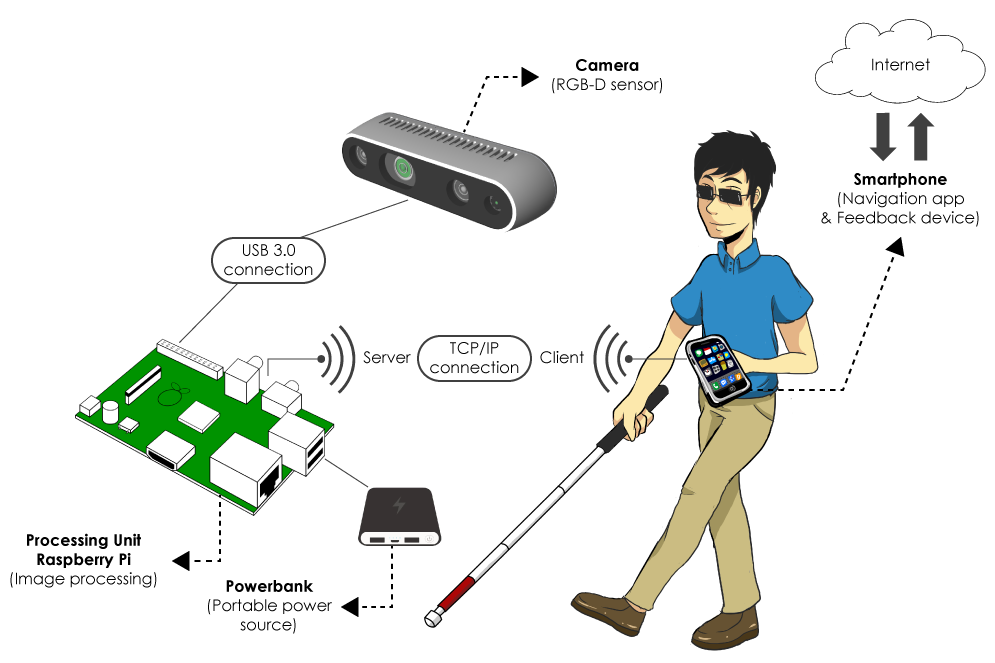
\includegraphics[width=\textwidth]{images/architecture.png}
    \caption{Αρχιτεκτονική προτεινόμενου συστήματος}
    \label{fig:architecture}
\end{figure}

Η αρχιτεκτονική του συστήματος πλοήγησης που προτείνεται στην παρούσα εργασία βασίζεται πάνω σε 3 κύριους πυλώνες:
\begin{itemize}
    \item \textbf{Μια κάμερα RGB-D με ενσωματωμένο αισθητήρα βάθους}: Στην λύση που προτείνουμε χρησιμοποιείται μια κάμερα ως μονάδα "αίσθησης" του εξωτερικού περιβάλλοντος μπροστά από τον χρήστη, η οποία έχει τη δυνατότητα καταγραφής βίντεο σε έγχρωμη μορφή (RGB) και παράλληλα δίνει ως έξοδο έναν χάρτη βάθους (depth map). Ουσιαστικά η κάμερα παίζει τον ρόλο των ματιών και δίνει την δυνατότητα υπολογισμού της απόστασης διαφόρων αντικειμένων από το άτομο με προβλήματα όρασης.
    \item \textbf{Ένα smartphone με εγκατεστημένη την εφαρμογή πλοήγησης}: Ως μέσο αλληλεπίδρασης του χρήστη με το σύστημα επιλέχθηκε το κινητό του. Ο λόγος είναι στην σημερινή εποχή η πλειοψηφία των ανθρώπων, ακόμα κι αυτών με προβλήματα όρασης, είναι εξοικειωμένοι με την χρήση ενός smartphone. Πρόκειται, δηλαδή, για μια συσκευή που ο καθένας έχει ανά πάσα στιγμή πάνω του και δεν προσθέτει επιπλέον φόρτο εργασίας στον χρήστη. Η εφαρμογή που αναπτύχθηκε στα πλαίσια της διπλωματικής εργασίας επιτρέπει στον χρήστη να εισάγει έναν προορισμό και η ίδια αναλαμβάνει την εύρεση της κατάλληλης διαδρομής, λαμβάνοντας υπόψιν την τωρινή τοποθεσία του χρήστη και τα δεδομένα από τους χάρτες πλοήγησης. Γίνεται αξιοποίηση του ενσωματωμένου GPS του κινητού και της εσωτερικής του πυξίδας, που περιλαμβάνει μαγνητόμετρο, γυροσκόπιο και επιταχυνσιόμετρο.
    \item \textbf{Την κύρια μονάδα επεξεργασίας εικόνας}: Για να λειτουργήσει ένα σύστημα πλοήγησης πρέπει να υπάρχει μια μονάδα η οποία θα λαμβάνει το βίντεο από την κάμερα και θα είναι υπεύθυνη για την επεξεργασία εικόνας που απαιτείται. Στην παρούσα εργασία επιλέχθηκε η χρήση ενός Raspberry Pi 4, το οποίο παρέχει την απαραίτητη επεξεργαστική ισχύ που απαιτείται για την επεξεργασία της ροής βίντεο, καθώς επίσης έχει και πολύ μικρό μέγεθος (λίγο μεγαλύτερο από πιστωτική κάρτα), που συμβάλλει στην φορητότητα του συστήματος. Πιο συγκεκριμένα, στο Raspberry Pi "τρέχουν" όλοι οι αλγόριθμοι εντοπισμού και αναγνώρισης εικόνας.
\end{itemize}

\subsection{Πλοήγηση σε αστικό περιβάλλον – δυσκολίες και περιορισμοί}
Όπως έχει ήδη αναφερθεί, στην παρούσα διπλωματική εργασία παρουσιάζεται ένα σύστημα πλοήγησης που προορίζεται για εξωτερικό χώρο και πιο συγκεκριμένα για αστικά περιβάλλοντα. Αν και οι δυσκολίες μετακίνησης είναι εξίσου έντονες και σε εσωτερικού χώρους, επιλέχθηκε η εστίαση σε εξωτερικά περιβάλλοντα, γιατί συνήθως αυτά είναι άγνωστα στους χρήστες και οι κίνδυνοι που μπορεί να αντιμετωπίσουν είναι πιο απρόβλεπτοι. Κατά την υλοποίηση του προτεινόμενου συστήματος πλοήγησης λήφθηκαν υπόψιν οι εξής παρατηρήσεις:
\begin{itemize}
    \item Ο εντοπισμός της θέσης του χρήστη είναι πιο εύκολος λόγω της διαθεσιμότητας του GPS. Αντίθετα, σε έναν εσωτερικό χώρο η χρήση του GPS είναι προβληματική λόγω χαμηλής στάθμης του σήματος.
    \item Σε ένα αστικό περιβάλλον, όπως μεγάλες πόλεις με ψηλά κτήρια, υπάρχει πιθανότητα να έχουμε ελάττωση της στάθμης σήματος του GPS, λόγω της παρεμβολής των κτιρίων. Αυτό οδηγεί συνήθως σε μειωμένη ακρίβεια του GPS, κάτι που είναι κρίσιμο για την πλοήγηση ενός ατόμου με μειωμένη όραση. Συχνά, αυτό το πρόβλημα εξαλείφεται με την κατασκευή όλο και καλύτερων δεκτών GPS, ή αλγοριθμικά με τη χρήση τεχνικών εντοπισμού θέσης μέσω της κάμερας που φέρει ο χρήστης. Στην παρούσα εργασία δεν θα ασχοληθούμε με την επίλυση του συγκεκριμένου ζητήματος, καθώς είναι κάτι που ξεφεύγει από τους στόχους.
    \item Κατά την πλοήγησή του ο χρήστης θα βρεθεί, συχνά, αντιμέτωπος με διάφορα φυσικά αντικείμενα, που λειτουργούν ως εμπόδια στην διαδρομή του. Επίσης, η ελλιπής συντήρηση των υποδομών, όπως η ύπαρξη σπασμένων πλακιδίων ή φυτών στα πεζοδρόμια και η έλλειψη ανάγλυφων οδηγών για τους τυφλούς, δυσχεραίνει την μετακίνησή των ατόμων αυτών.
    \item Τέλος, τα συστήματα πλοήγησης που βασίζονται σε κάμερες ή αισθητήρες υπερύθρων, επηρεάζονται από τις ακτίνες του ήλιου, οι οποίες δημιουργούν παρεμβολές και περιορίζουν την εφαρμοσιμότητα των αλγορίθμων.
\end{itemize}

\subsection{Παράλληλη χρήση με το λευκό μπαστούνι}
Αν και η τεχνολογία έχει πραγματοποιήσει τεράστια άλματα προόδου τις τελευταίες δεκαετίες, είναι γεγονός πως δεν έχει σχεδιαστεί κάποια εφαρμογή πλοήγησης για τυφλούς που να ικανοποιεί τις ανάγκες τους πλήρως και να αντικαταστήσει τις παραδοσιακές μεθόδους υποβοήθησης πλοήγησης \cite{LowVisio34:online}. Συνεπώς, η κοινότητα των ατόμων με προβλήματα όρασης εξακολουθεί δικαίως να χρησιμοποιεί το λευκό μπαστούνι, ως το κύριο βοήθημα μετακίνησης, κάτι το οποίο δεν μπορεί να αλλάξει από τη μια στιγμή στην άλλη. Για αυτόν τον λόγο, το σύστημα που παρουσιάζεται στην παρούσα εργασία προορίζεται να λειτουργεί υποστηρικτικά στη χρήση του λευκού μπαστουνιού, βελτιώνοντας ταυτόχρονα την εμπειρία μετακίνησης των χρηστών και επιτρέποντάς τους την χρήση των εργαλείων που εμπιστεύονται και με τα οποία έχουν εξοικειωθεί.

\section{Απτική Ανάδραση}
\subsection{Αισθητηριακή υποκατάσταση}
Η έννοια της αισθητηριακής υποκατάστασης (sensory substitution) αναφέρεται στην τροποποίηση ορισμένων χαρακτηριστικών ενός αντιληπτικού συστήματος (π.χ. όραση, ακοή, αφή, όσφρηση, γεύση) και η μετατροπή τους σε ερεθίσματα για ένα διαφορετικό αντιληπτικό σύστημα \cite{wiki:sensory_sub}. Με άλλα λόγια, η κεντρική ιδέα της αισθητηριακής υποκατάστασης είναι ότι οι πληροφορίες, οι οποίες δεν είναι διαθέσιμες σε κάποιον εξαιτίας μιας αισθητηριακής διαταραχής, μπορούν να γίνουν αντιληπτές μέσω ενός άλλου αντιληπτικού συστήματος. Η μετατροπή, ωστόσο, των ερεθισμάτων από ένα αντιληπτικό σύστημα σε ένα άλλο είναι μια πολύπλοκη διαδικασία με πολλές παραμέτρους, η οποία αποτελεί αντικείμενο έρευνας τόσο στον ιατρικό όσο και στον τεχνολογικό τομέα. Στα πλαίσια της διπλωματικής εργασίας θα αξιοποιήσουμε πολύ βασικές γνώσεις που αφορούν την αντικατάσταση μιας αίσθησης με μια άλλη, χωρίς να εμβαθύνουμε περαιτέρω.

\subsection{Υπάρχοντα κανάλια μετάδοσης χωρικής πληροφορίας}
Οι άνθρωποι με φυσιολογική όραση χρησιμοποιούν την όραση για να προσδιορίσουν την θέση τους και το μονοπάτι στο οποίο θα κινηθούν. Τα άτομα με προβλήματα όρασης έχουν αναπτύξει τις υπόλοιπες αισθήσεις τους ώστε να μπορούν να αντιλαμβάνονται τον χώρο στον οποίο βρίσκονται. Όπως είναι φυσιολογικό τα δύο αισθητήρια κανάλια που αξιοποιούνται περισσότερο είναι το ακουστικό και το απτικό, το οποίο έχει επιβεβαιωθεί κι από αντίστοιχες έρευνες \cite{schmidt2013spatial}. Χρησιμοποιώντας το ακουστικό κανάλι τα άτομα με προβλήματα όρασης είναι σε θέση να αντιλαμβάνονται τις αλλαγές που συμβαίνουν γύρω τους και να προσανατολίζονται, χρησιμοποιώντας διάφορες πηγές ήχου ως σημεία αναφοράς, π.χ. ο θόρυβος που κάνουν τα οχήματα τους επιτρέπει να γνωρίζουν πού βρίσκεται ο δρόμος, ενώ η ηχητική ειδοποίηση των φαναριών τους βοηθάει να καταλάβουν αν είναι πράσινο ή κόκκινο. Αντίθετα, η χωρική πληροφορία είναι δύσκολο να μεταφερθεί άμεσα μέσω του απτικού καναλιού. Η χρησιμότητά του είναι ότι μέσω της αφής ο χρήστης αντιλαμβάνεται περισσότερες λεπτομέρειες σχετικά με την υφή ή το είδος ενός φυσικού αντικειμένου. Για παράδειγμα, όταν ο τυφλός χρησιμοποιεί το λευκό μπαστούνι και αυτό πέσει πάνω σε ένα εμπόδιο, τότε, αναλόγως την δύναμη που ασκείται στον μπαστούνι, μπορεί να αντιληφθεί αν το αντικείμενο αυτό είναι κάτι σκληρό και αμετακίνητο (π.χ. μια κολόνα δημοτικού φωτισμού), ή κάτι πιο εύκαμπτο και μετακινήσιμο (π.χ. μια καρέκλα).

\subsection{Γιατί απτική ανάδραση;}
Στην παρούσα διπλωματική εργασία υλοποιείται ένα σύστημα υποβοήθησης πλοήγησης που βασίζεται στην απτική αλληλεπίδραση με τον χρήστη. Πιο συγκεκριμένα, υλοποιήθηκε ένα σύστημα που ειδοποιεί τον χρήστη μέσω δονήσεων για το πότε και πού πρέπει να κινηθεί, καθώς επίσης και όταν απαιτείται η διάσχιση ενός δρόμου. Η επιλογή του απτικού καναλιού ως μέσο μετάδοσης της χωρικής πληροφορίας έγινε για τους εξής δύο λόγους:
\begin{enumerate}
    \item Το ακουστικό κανάλι είναι ήδη αρκετά επιβαρυμένο με άλλες λειτουργίες \cite{bharadwaj2017tactile, shingledecker1978human} και απαιτείται μια αποσυμφόρηση, ώστε το άτομο με προβλήματα όρασης να μπορεί να αντιλαμβάνεται άλλες κρίσιμες πληροφορίες μέσω της ακοής, π.χ. τον ήχο από τα αυτοκίνητα ή κάποιον περαστικό. Επίσης, η παροχή ανάδρασης μέσω ήχου θα μπορούσε να συγχύσει και να κουράσει πνευματικά τον χρήστη, λόγω πολλών παράλληλων ακουστικών ερεθισμάτων.
    \item Η χρήση δονήσεων αποτελεί έναν πιο διακριτικό τρόπο να ενημερώνεται ο χρήστης για πληροφορίες που αφορούν το εξωτερικό περιβάλλον. Η διακριτικότητα και η ευκολία είναι από τα βασικά χαρακτηριστικά του προτεινόμενου συστήματος και η αξιοποίηση του απτικού καναλιού είναι απαραίτητη για να επιτευχθεί κάτι τέτοιο.
\end{enumerate}

\subsection{Haptic icons}
Ως haptic icons ορίζονται στην βιβλιογραφία τα διάφορα απτά ερεθίσματα στα οποία έχουμε αποδώσει συγκεκριμένα νοήματα (π.χ. ένα απτικό ερέθισμα μπορεί να είναι "συνδεδεμένο" με την έκφραση χαράς, λύπης κλπ.) \cite{chan2008designing}. Σχετικές έρευνες \cite{seifi2017exploiting, shieh2008tactile} έχουν μελετήσει τη σχέση μεταξύ των απτικών ερεθισμάτων που δέχεται ένας άνθρωπος και των συναισθημάτων που του προκαλούν. Συνήθως συστήματα που βασίζονται στην αξιοποίηση του απτικού καναλιού στοχεύουν στην μετάδοση πληροφοριών στον χρήστη μέσω της χρήσης διαφορετικών μοτίβων δονήσεων, τα οποία είναι συνδεδεμένα με διαφορετικές εντολές πλοήγησης. Τα διαφορετικά μοτίβα δονήσεων μπορεί να περιλαμβάνουν διαφορές στην ένταση της δόνησης, στην αλληλουχία των δονήσεων και στην συχνότητά τους. Για τις ανάγκες της συγκεκριμένης διπλωματικής εργασίας χρησιμοποιήθηκε η λογική της αντιστοίχησης ενός μοτίβου δονήσεων, τα οποία παίζουν τον ρόλο των haptic icons, για κάθε διαφορετική εντολή που απαιτείται από τον χρήστη. Κάθε μοτίβο έχει το ίδιο επίπεδο έντασης, καθώς θεωρήθηκε ότι ο αριθμός των εντολών που έπρεπε να κωδικοποιηθούν δεν ήταν τόσο μεγάλος, ώστε να αξιοποιηθεί και η ένταση των δονήσεων για περισσότερη διακριτοποίηση. Πιο συγκεκριμένα:
\begin{itemize}
    \item Εντολή \textbf{"Στρίψε Αριστερά"}: Η εντολή αυτή ειδοποιεί τον χρήστη ότι πρέπει να πραγματοποιήσει στροφή αριστερά 90\degree. Το μοτίβο δονήσεων που αντιστοιχεί σε αυτήν την εντολή είναι "σύντομη δόνηση - μικρή παύση - σύντομη δόνηση".
    \item Εντολή \textbf{"Στρίψε Δεξιά"}: Η εντολή αυτή ειδοποιεί τον χρήστη ότι πρέπει να πραγματοποιήσει στροφή δεξιά 90\degree. Το μοτίβο δονήσεων που αντιστοιχεί σε αυτήν την εντολή είναι "μακρά δόνηση - μικρή παύση - μακρά δόνηση".
    \item Εντολή \textbf{"Σταμάτα"}: Η εντολή αυτή ειδοποιεί τον χρήστη ότι πρέπει να σταματήσει μπροστά από μια διάβαση, επειδή το ο φωτεινός σηματοδότης είναι κόκκινος. Το μοτίβο δονήσεων που αντιστοιχεί σε αυτήν την εντολή είναι "πολύ μακρά δόνηση - πολύ σύντομη παύση".
    \item Εντολή \textbf{"Προχώρα"}: Η εντολή αυτή ειδοποιεί τον χρήστη ότι μπορεί να διασχίσει μια διάβαση, επειδή το ο φωτεινός σηματοδότης είναι πράσινος. Το μοτίβο δονήσεων που αντιστοιχεί σε αυτήν την εντολή είναι "σύντομη δόνηση - πολύ σύντομη παύση - μακρά δόνηση - πολύ σύντομη παύση".
\end{itemize}
\begin{figure}[H]
    \centering
    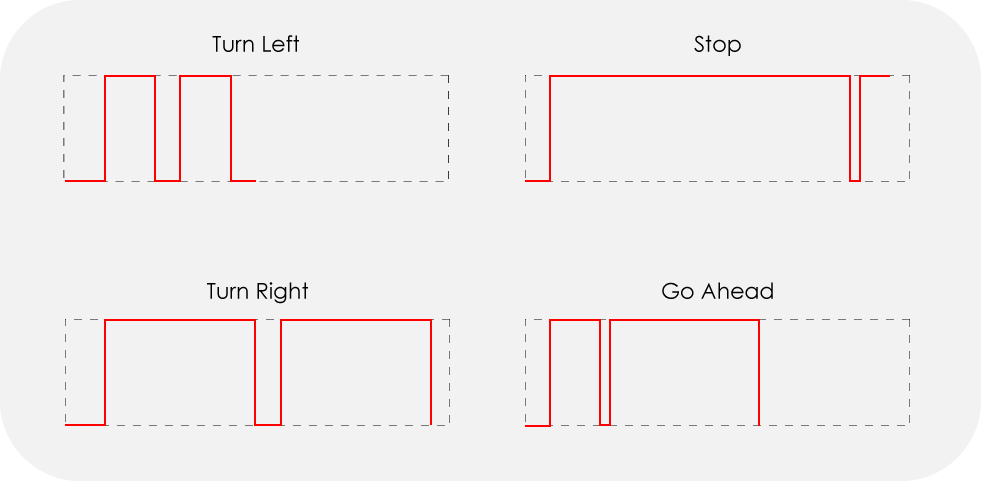
\includegraphics[width=\textwidth]{images/haptic_icons.png}
    \caption{Αντιστοίχηση μοτίβων δονήσεων σε εντολές πλοήγησης}
    \label{fig:haptic-icons}
\end{figure}

\subsection{Δυνατότητες και περιορισμοί}
Όπως έχουμε ήδη αναφέρει η χρήση της αφής ως μέσο μετάδοσης πληροφορίας έχει πολύ μεγάλο πλεονέκτημα την διακριτικότητα και την αμεσότητα στην αντίληψη της πληροφορίας. Ωστόσο, συγκριτικά με την ακοή, προβάλει ένα σημαντικό μειονέκτημα, το οποίο είναι η χαμηλή διακριτότητα της πληροφορίας που μπορεί να μεταδοθεί \cite{kaczmarek1991electrotactile}. Με απλά λόγια, αν θέλουμε να κωδικοποιήσουμε πολλές διαφορετικές εντολές με χρήση μοτίβων δονήσεων, τότε θα πρέπει να δημιουργήσουμε ένα διαφορετικό μοτίβο για κάθε ξεχωριστή εντολή. Ωστόσο, η δυνατότητα του ανθρώπου να αντιλαμβάνεται διαφορετικά μοτίβα δονήσεων με μικρές διαφορές μεταξύ τους μειώνεται όσο αυξάνεται η πολυπλοκότητα και ο αριθμός αυτών των μοτίβων. Έρευνες έχουν δείξει επίσης, ότι η διακριτότητα της πληροφορίας που μπορεί να αντιληφθεί ένα άνθρωπος μέσω της αφής εξαρτάται από το σημείο του δέρματος που δέχεται τη διέγερση, για παράδειγμα τα δάκτυλα έχουν πολύ μεγαλύτερη δυνατότητα διάκρισης σε σχέση με τον αγκώνα. Το κατώφλι διάκρισης μεταξύ δυο σημείων (two-point discrimination threshold (TPDT)) ορίζεται ως το μέτρο το οποίο αναπαριστά πόσο πρέπει να απέχουν δυο σημεία πίεσης ώστε να θεωρηθούν από το δέρμα ως διακριτά \cite{koo2016two}.
\begin{figure}[H]
    \centering
    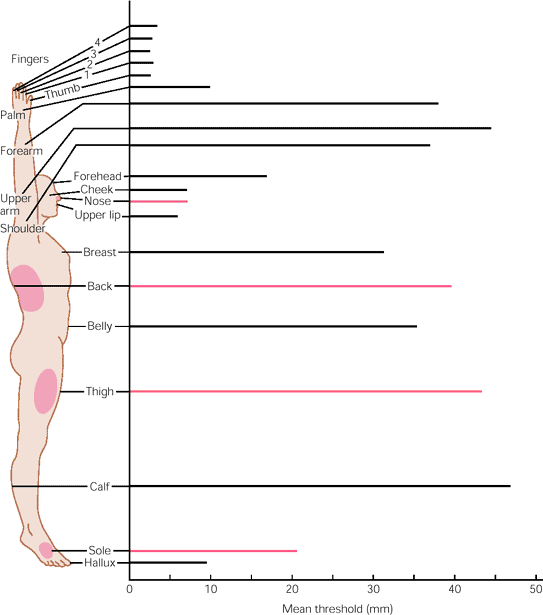
\includegraphics[width=0.6\textwidth]{images/TPDT.png}
    \caption{Μεταβολή του TPDT σε συνάρτηση με τα σημεία του σώματος \cite{weinstein1968intensive}}
    \label{fig:TPDT}
\end{figure}
\newpage
\section{Εξοπλισμός - Υλικό (Hardware)}
Στην ενότητα αυτή θα γίνει μια πλήρης περιγραφή του εξοπλισμού που χρησιμοποιήθηκε στα πλαίσια της παρούσας διπλωματικής εργασίας.

\subsection{Μονάδα «αίσθησης» του περιβάλλοντος – Camera/Depth Sensor}
\subsubsection{Διαθέσιμοι αισθητήρες}
Υπάρχουν πολλοί διαθέσιμοι αισθητήρες-κάμερες που θα μπορούσαν να αξιοποιηθούν στα πλαίσια ενός συστήματος πλοήγησης για άτομα με προβλήματα όρασης. Η επιλογή του κατάλληλου αισθητήρα εξαρτάται κυρίως από τις ανάγκες τις εκάστοτε εφαρμογής, π.χ. αν πρόκειται για εξωτερικό ή εσωτερικό περιβάλλον κλπ. Στην παρούσα εργασία χρησιμοποιήσαμε την κάμερα \emph{Intel Realsense D435i}, ωστόσο πριν προχωρήσουμε στην τελική επιλογή κάμερας εξετάσαμε τις εξής εναλλακτικές επιλογές:
\begin{itemize}
    \item \emph{ZED Stereo Camera}: Πρόκειται για μια κάμερα που λειτουργεί με την μέθοδο της στερεοσκοπικής όρασης, δηλαδή χρησιμοποιεί δύο διαφορετικούς φακούς με οριζόντια απόσταση ο ένας από τον άλλο, και το βάθος/απόσταση υπολογίζεται συγκρίνοντας την μετατόπιση των δύο διαφορετικών εικόνων.
    \begin{table}[H]
    \centering
    \begin{tabular}{|c|c|}
        \hline
        Technology: & Stereo Depth Sensing\\
        \hline
        Field of View (FoV): & Max. 90°(H) x 60°(V) x 100°(D)\\
        \hline
        RGB Sensor Type: & 1/3” 4MP CMOS\\
        \hline
        Depth Range: & 0.5m to 25m\\
        \hline
        Depth FPS: & Up to 100Hz\\
        \hline
        Depth Accuracy: & <= 2\% up to 3m, <= 4\% up to 15m\\
        \hline
        Dimensions: & 175 x 30 x 33 mm\\ 
        \hline
        Power: & 380mA / 5V USB Powered\\
        \hline
        SDK Provided: & YES\\
        \hline
    \end{tabular}
    \caption{Χαρακτηριστικά ZED Stereo Camera \cite{ZEDStere94:online}}
    \label{tab:zed}
    \end{table}
    \begin{figure}[H]
        \centering
        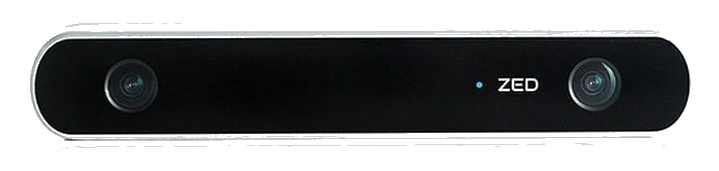
\includegraphics[width=0.6\textwidth]{images/zed.png}
        \caption{ZED Stereo Camera}
        \label{fig:zed}
    \end{figure}

    \item \emph{CamBoard pico flexx depth sensor}: Ο αισθητήρας αυτός είναι από τους πιο μικρούς που υπάρχουν και χρησιμοποιεί την τεχνολογία Time-of-Flight (ToF), με εκπομπή υπέρυθρης ακτινοβολίας, για να υπολογίσει την απόσταση των αντικειμένων, χωρίς ωστόσο να παρέχει δυνατότητα RGB εικόνας.
    \begin{table}[H]
    \centering
    \begin{tabular}{|c|c|}
        \hline
        Technology: & Time-of-Flight (ToF)\\
        \hline
        Field of View (FoV): & Max. 62°(H) x 45°(V)\\
        \hline
        RGB Sensor Type: & Δεν υποστηρίζεται\\
        \hline
        Depth Range: & 0.1m to 4m\\
        \hline
        Depth FPS: & Up to 45fps\\
        \hline
        Depth Accuracy: & <= 1\% of distance (0.5 – 4m @ 5fps), <= 2\% of distance (0.1 – 1m @ 45fps)\\
        \hline
        Dimensions: & 68 x 17 x 7.35 mm\\ 
        \hline
        Power: & 300mW / USB2.0 compliant\\
        \hline
        SDK Provided: & YES\\
        \hline
    \end{tabular}
    \caption{Χαρακτηριστικά CamBoard pico flexx depth sensor \cite{CamBoard10:online}}
    \label{tab:pico}
    \end{table}
    \begin{figure}[H]
        \centering
        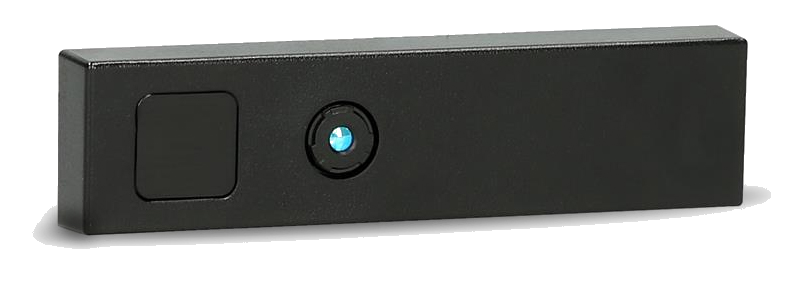
\includegraphics[width=0.6\textwidth]{images/pico_flexx.png}
        \caption{CamBoard pico flexx depth sensor}
        \label{fig:pico}
    \end{figure}
\end{itemize}

\subsubsection{Κριτήρια επιλογής κατάλληλου αισθητήρα}
Η επιλογή του κατάλληλου αισθητήρα έγινε λαμβάνοντας υπόψιν τα παρακάτω κριτήρια:
\begin{enumerate}
    \item \emph{Διαστάσεις κάμερας}: Στόχος είναι η φορητότητα και η διακριτικότητα του συστήματος, άρα θέλουμε έναν όσο γίνεται μικρότερο σε διαστάσεις αισθητήρα.
    \item \emph{Ταυτόχρονη υποστήριξη RGB \& Depth Frames}: Η προτεινόμενη εφαρμογή αξιοποιεί τόσο την έγχρωμη εικόνα RGB για την αναγνώριση της διάβασης πεζών και των φωτεινών σηματοδοτών, όσο και τον χάρτη βάθους (depth map) για τον εντοπισμό φυσικών εμποδίων.
    \item \emph{Ανθεκτικότητα στις συνθήκες φωτισμού}: Λόγω της φύσης του συστήματος, είναι απαραίτητο η κάμερα να αποδίδει επαρκώς καλά τόσο σε εσωτερικά, όσο και σε εξωτερικά περιβάλλοντα. Ιδιαίτερα η ακρίβεια των μετρήσεων της κάμερας σε εξωτερικό περιβάλλον επηρεάζεται από τον φωτισμό του περιβάλλοντος και τον προσανατολισμό της σε σχέση με τις ακτίνες του ήλιου. 
    \item \emph{Επαρκή υποστήριξη με SDK (Software Development Kit)}: Κατά την υλοποίηση μιας εργασίας είναι πολύ σημαντικό να υπάρχουν διαθέσιμα παραδείγματα κώδικα και έτοιμες συναρτήσεις που διευκολύνουν την ανάπτυξη των αλγορίθμων. Τα SDKs είναι πακέτα λογισμικού, που περιέχουν βελτιστοποιημένες συναρτήσεις και βασικά παραδείγματα για την ορθή χρήση του εκάστοτε αισθητήρα. Η ύπαρξη μιας ευρύτερης κοινότητας γύρω από έναν συγκεκριμένο αισθητήρα συμβάλλει στην πιο γρήγορη και αποτελεσματική υλοποίηση, καθώς και στην πιο εύκολη επίλυση των σφαλμάτων.
    \item \emph{Ακρίβεια και εύρος μέτρησης απόστασης}: Η ακρίβεια κατά την μέτρηση των αποστάσεων, καθώς και το εύρος της μέτρησης (ελάχιστη/μέγιστη μετρήσιμη απόσταση) είναι κρίσιμα κριτήρια για την επιλογή του κατάλληλου αισθητήρα βάθους, ο οποίος θα καλύπτει τις ανάγκες ενός πεζού χρήστη με προβλήματα όρασης.
\end{enumerate}

\subsubsection{Intel RealSense D435i}
Στα πλαίσια της παρούσας διπλωματικής εργασίας χρησιμοποιήθηκε η κάμερα \emph{Intel Realsense D435i}, η οποία περιέχει έναν RGB φακό και έναν ενσωματωμένο αισθητήρα βάθους, ο οποίος λειτουργεί με στερεοσκοπική όραση. Η αρχή λειτουργίας της στερεοσκοπικής όρασης είναι παρόμοια με τον τρόπο που αντιλαμβάνεται το βάθος ο ανθρώπινος εγκέφαλος μέσω των ματιών, δηλαδή υπάρχουν δύο φακοί-αισθητήρες τοποθετημένοι σε μικρή απόσταση μεταξύ τους και λαμβάνουν δύο διαφορετικές εικόνες ενός αντικειμένου. Συγκρίνοντας τις δύο εικόνες και γνωρίζοντας την απόσταση μεταξύ των δύο φακών εξάγεται η πληροφορία που αφορά το βάθος (Σχήμα \ref{fig:stereo}). Οι στερεοσκοπικές κάμερες λειτουργούν αρκετά καλά κάτω από οποιεσδήποτε συνθήκες φωτισμού, αφού το βάθος υπολογίζεται αποκλειστικά από την σύγκριση εικόνων. Η κάμερα Intel Realsense D435i χρησιμοποιεί επιπλέον έναν πομπό υπέρυθρης ακτινοβολίας (infrared projector), ώστε έχει μεγαλύτερη ακρίβεια μετρήσεων σε περιβάλλοντα χαμηλού φωτισμού. Τέλος, ενσωματώνει κι έναν IMU (Inertial Measurement Sensor) sensor, έναν αισθητήρα που περιλαμβάνει επιταχυνσιόμετρο και γυροσκόπιο, για να μετράει την περιστροφή και τον προσανατολισμό της κάμερας με 6 βαθμούς ελευθερίας.

\begin{figure}[H]
        \centering
        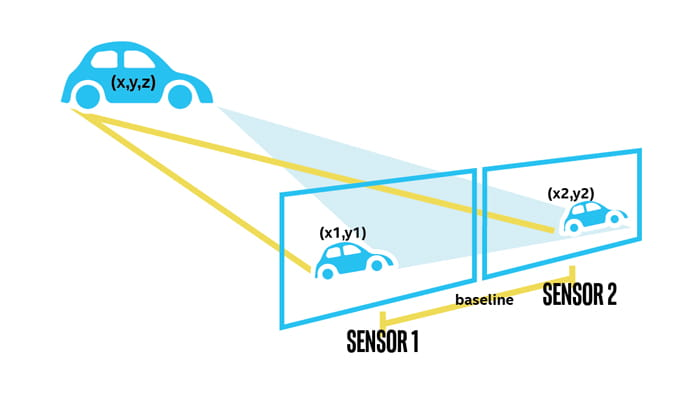
\includegraphics[width=0.8\textwidth]{images/how_stereo_depth_works.jpg}
        \caption{Αρχή λειτουργίας στερεοσκοπικής όρασης}
        \label{fig:stereo}
    \end{figure}

\begin{table}[H]
    \centering
    \begin{tabular}{|c|c|}
        \hline
        Technology: & Active IR Stereo\\
        \hline
        Field of View (FoV): & Max. 90°(H) x 59°(V) x 98°(D)\\
        \hline
        RGB Sensor: & 1920 x 1080, 30fps\\
        \hline
        Depth Range: & 0.105m to 10m\\
        \hline
        Depth FPS: & Up to 90fps\\
        \hline
        Dimensions: & 90 x 25 x 25 mm\\ 
        \hline
        Power: & USB3.0\\
        \hline
        SDK Provided: & YES\\
        \hline
    \end{tabular}
    \caption{Χαρακτηριστικά Intel Realsense D435i \cite{DepthCam34:online}}
    \label{tab:realsense}
\end{table}
\begin{figure}[H]
    \centering
    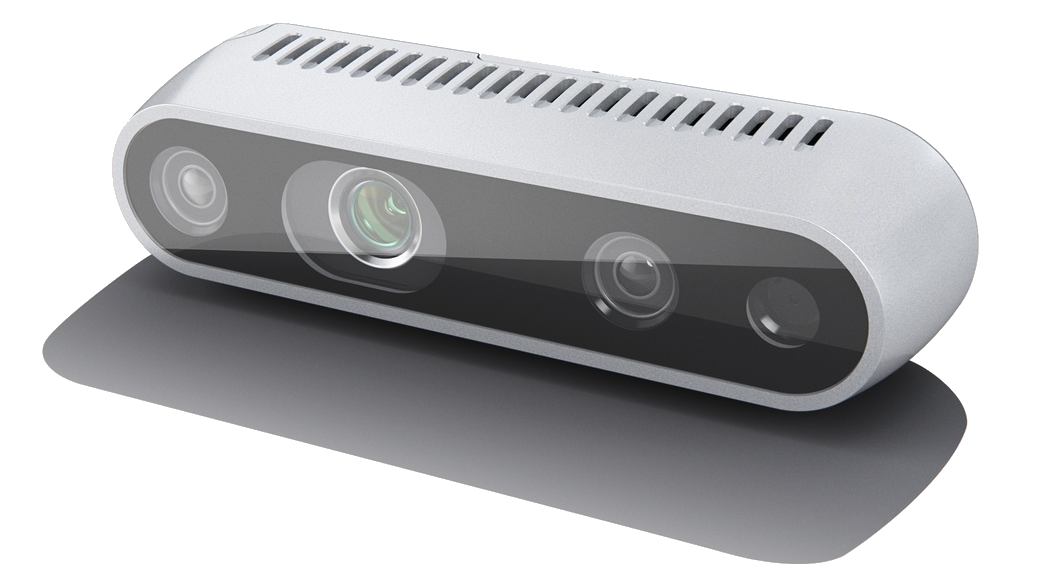
\includegraphics[width=0.8\textwidth]{images/intel_realsense.png}
    \caption{Intel Realsense Depth Camera D435i}
    \label{fig:realsense}
\end{figure}
\begin{figure}[H]
    \centering
    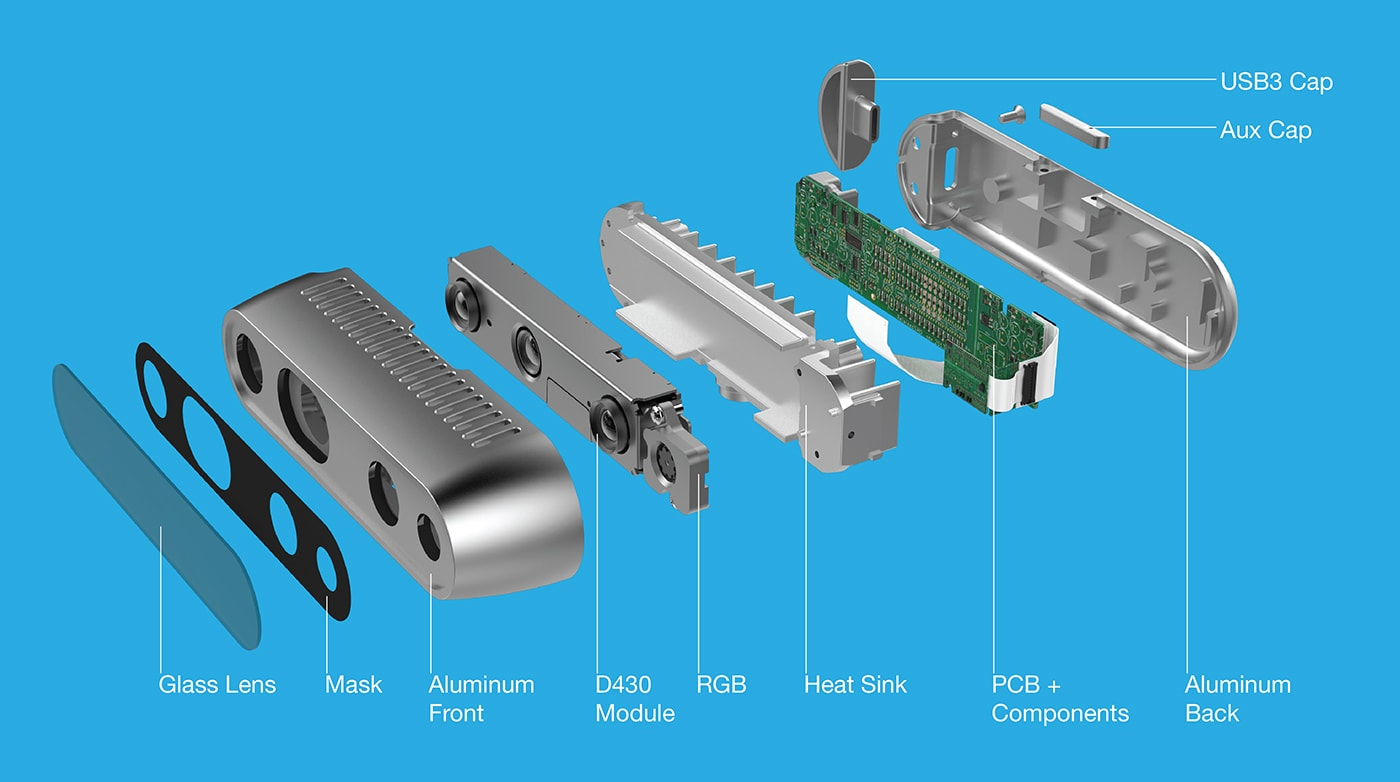
\includegraphics[width=\textwidth]{images/d435_inside_depth_camera.jpg}
    \caption{Intel Realsense D435i - Εσωτερική δομή}
    \label{fig:realsense-inside}
\end{figure}

\subsection{Μονάδα επεξεργασίας εικόνας – Μικροϋπολογιστής}
Οι αλγόριθμοι εντοπισμού και αναγνώρισης αντικειμένων χρησιμοποιούν τεχνικές επεξεργασίας εικόνας για να καταφέρουν να αποκωδικοποιήσουν μια φωτογραφία ή ένα βίντεο. Η επεξεργασία εικόνας και βίντεο είναι μια απαιτητική εργασία τόσο σε μνήμη όσο και σε επεξεργαστική ισχύ, επομένως είναι απαραίτητη η ύπαρξη ενός υπολογιστή ή κάποιας μονάδας επεξεργασίας που θα μπορεί να αντεπεξέλθει στις απαιτήσεις αυτές.

\subsubsection{Raspberry Pi 4}
\begin{figure}[H]
    \centering
    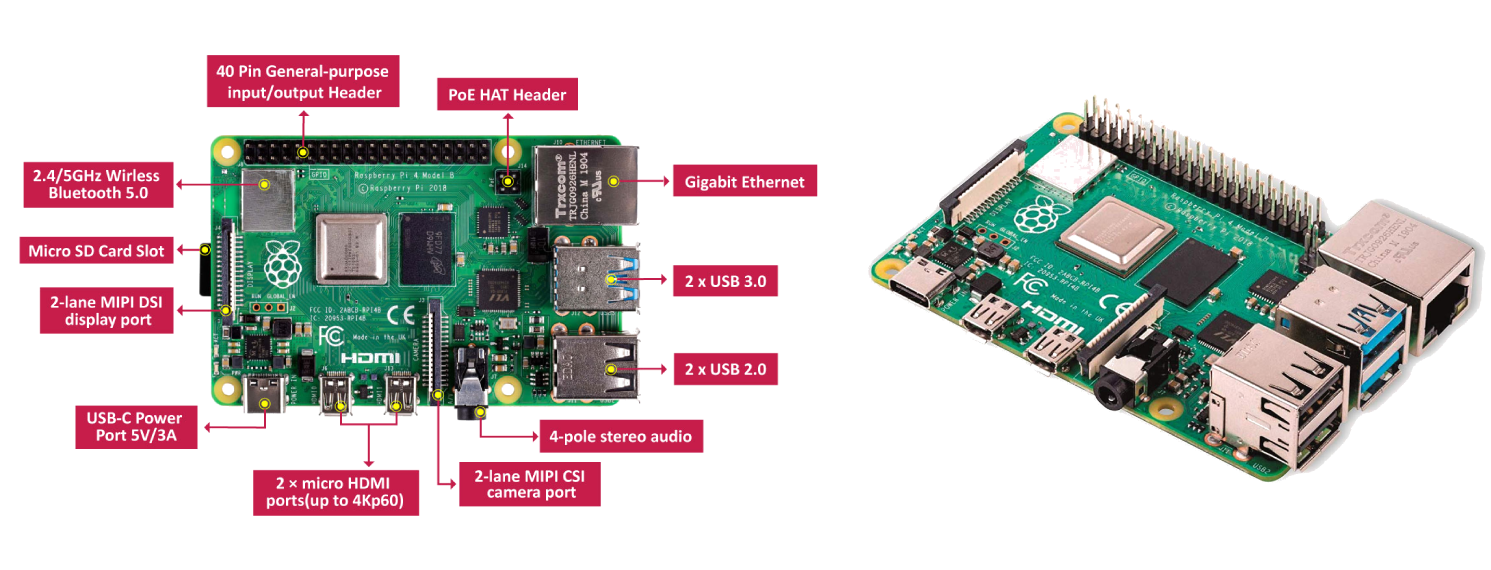
\includegraphics[width=\textwidth]{images/raspberry.png}
    \caption{Raspberry Pi 4 Model B}
    \label{fig:RPi4modelB}
\end{figure}
Για τις ανάγκες της διπλωματικής εργασίας επιλέχθηκε η χρήση του μικροεπεξεργαστή \emph{Raspberry Pi 4} (RPi4). Το RPi4 είναι ένας πλήρης υπολογιστής σε μέγεθος πιστωτικής κάρτας, στον οποίο μπορούν να συνδεθούν διάφορες περιφερειακές συσκευές, όπως πληκτρολόγιο, οθόνη κλπ. Πιο συγκεκριμένα, χρησιμοποιήθηκε η έκδοση Model B του Raspberry Pi 4, το οποίο έχει βελτιωμένα χαρακτηριστικά, όπως υποστήριξη USB3.0, μεγαλύτερη μνήμη RAM (4GB) και καλύτερο επεξεργαστή γραφικών. Στον πίνακα \ref{tab:raspberry} παρουσιάζονται αναλυτικά τα χαρακτηριστικά του Raspberry Pi 4 που χρησιμοποιήσαμε.

\begin{table}[H]
    \centering
    \begin{tabular}{|c|c|}
        \hline
        Processor: & Broadcom BCM2711, quad-core Cortex-A72 (ARM v8)
64-bit SoC @ 1.5GHz\\
        \hline
        Memory: & 4GB LPDDR4\\
        \hline
        Connectivity: & WLAN, Ethernet, Bluetooth 5.0, BLE\\
        \hline
        USB2.0: & 2 ports\\
        \hline
        USB3.0: & 2 ports\\
        \hline
        HMDI: & 2 micro HDMI ports\\
        \hline
        Micro SD: & YES\\
        \hline
        Input power: & 5V DC via USB-C connector (minimum 3A)\\
        \hline
    \end{tabular}
    \caption{Χαρακτηριστικά Raspberry Pi 4 Model B \cite{BuyaRasp17:online}}
    \label{tab:raspberry}
\end{table}

Ουσιαστικά, στα πλαίσια της παρούσας εργασίας αξιοποιήθηκαν κυρίως η μεγάλη χωρητικότητα μνήμης RAM και η ύπαρξη θύρας USB3.0, μιας και η κάμερα που επιλέξαμε υποστήριζε αποκλειστικά USB3.0 interface. Ταυτόχρονα, η μεγάλη επεξεργαστική ισχύς συνέβαλε στο να τρέχει ο αλγόριθμος σε real-time, ενώ η WiFi συνδεσιμότητα επέτρεψε την σύνδεση με τα άλλα μέρη του συστήματος, όπως θα δούμε παρακάτω. Η τροφοδοσία του RPi4 μπορεί να γίνει με δύο τρόπους: είτε με μια συστοιχία από μπαταρίες ιόντων λιθίου, είτε μέσω ενός powerbank (φορητή μπαταρία). Επιλέχθηκε η δεύτερη λύση του powerbank, καθώς ήταν πολύ πιο εύκολο να το αποκτήσουμε και δεν απαιτεί ιδιαίτερους χειρισμούς όσον αφορά την επαναφόρτισή του. Το RPi4 απαιτεί τροφοδοσία 5V/3A, επομένως χρησιμοποιήθηκε ένα powerbank που έχει ως έξοδο 5V/3A και χωρητικότητα μπαταρίας 10.000mAh (Σχήμα \ref{fig:powerbank}). Η αυτονομία του συστήματος με την χρήση της συγκεκριμένης φορητής μπαταρίας φτάνει έως και την 1.5 ώρα.

\begin{figure}[H]
    \centering
    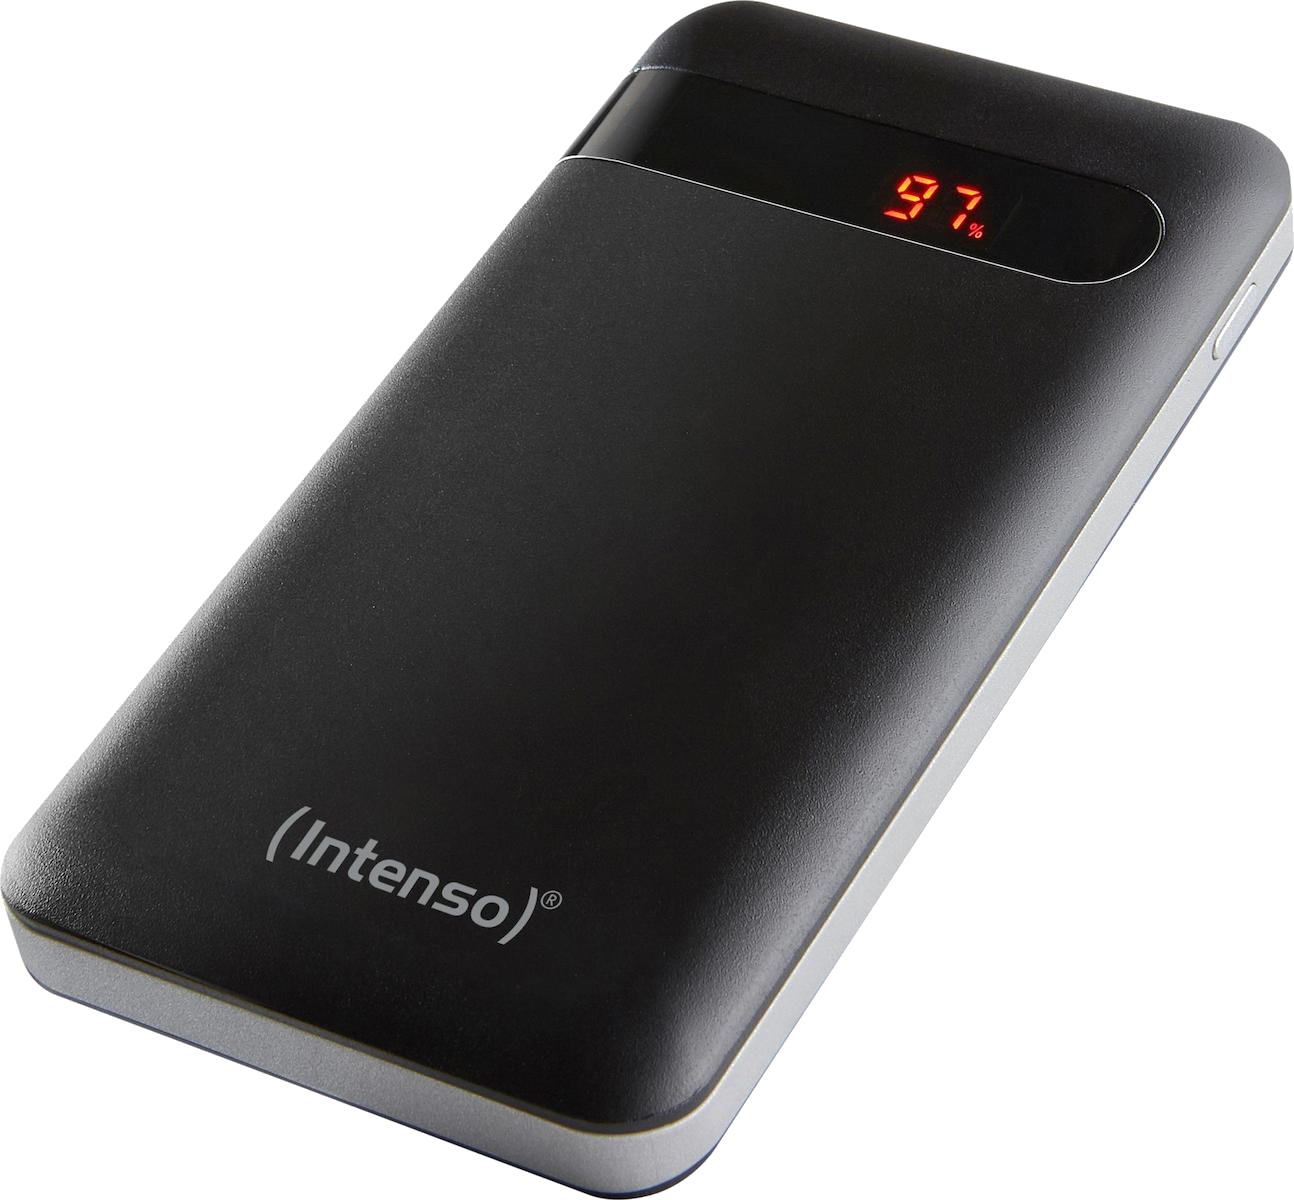
\includegraphics[width=0.6\textwidth]{images/powerbank.png}
    \caption{Το powerbank \emph{Intenso PD10000} που χρησιμοποιήθηκε}
    \label{fig:powerbank}
\end{figure}

\subsection{Συσκευή πλοήγησης – Android Smartphone}
Η επιλογή του κινητού του χρήστη ως κύρια συσκευή πλοήγησης έγινε, διότι πρόκειται για μια συσκευή με την οποία οι χρήστες είναι αρκετά εξοικειωμένοι, είναι άμεσα διαθέσιμη σχεδόν σε όλους και είναι πολύ εύκολο να αναπτυχθούν εφαρμογές για smartphone.

\subsubsection{Εφαρμογή πλοήγησης}
Στα πλαίσια της διπλωματικής αναπτύχθηκε ειδική εφαρμογή για κινητά σε λειτουργικό Android. Η εφαρμογή προορίζεται να εγκαθίσταται στο κινητό του χρήστη και αποτελεί την μοναδική διεπιφάνεια αλληλεπίδρασης του χρήστη με το σύστημα πλοήγησης. Το κομμάτι της υλοποίησης της εφαρμογής περιλαμβάνει την ανάπτυξη κώδικα που αξιοποιεί τους ενσωματωμένους αισθητήρες GPS, IMU και πυξίδα για να μπορεί να εντοπίζεται η τοποθεσία του χρήστη.
\newline
\newline
\textbf{Αρχή λειτουργίας}:

Η εφαρμογή ενσωματώνει έναν χάρτη της ευρύτερης περιοχής χάρη στη χρήση του \emph{Google Maps SDK} \url{https://developers.google.com/maps/documentation/android-sdk/intro}.
Ο χρήστης εισάγει έναν προορισμό στην εφαρμογή και η αντίστοιχη τοποθεσία βρίσκεται μέσω του \emph{Google Places API} (\url{https://developers.google.com/places/web-service/intro}).
Αφού ο χρήστης εισάγει έναν προορισμό, το σύστημα βρίσκει την βέλτιστη διαδρομή, χρησιμοποιώντας το \emph{Google Directions API} (\url{https://developers.google.com/maps/documentation/directions/intro}) και επιστρέφονται ως δεδομένα οι οδηγίες κατεύθυνσης για πεζούς. Το format των οδηγιών είναι JSON, οπότε αναπτύχθηκε μια εσωτερική συνάρτηση στην εφαρμογή που αποκωδικοποιεί τα δεδομένα κατεύθυνσης και τα εξάγει ως μια λίστα από απλές εντολές στροφής (turn-by-turn navigation).
Καθόσον η εφαρμογή βρίσκεται σε λειτουργία πυξίδας, επικοινωνεί με το Raspberry Pi ασύρματα και λαμβάνει εντολές για το αν έχει βρεθεί κάποιο εμπόδιο ή έχει εντοπιστεί διάβαση πεζών. Η εφαρμογή αντιλαμβάνεται τον προσανατολισμό του χρήστη εκμεταλλευόμενη τους εσωτερικούς αισθητήρες του κινητού και υπολογίζει την γωνία απόκλισης που έχει σε σχέση με τον προσανατολισμό του μονοπατιού που ακολουθεί. Αν η απόκλιση είναι μεγαλύτερη των 30\degree (σχήμα \ref{fig:degree-orientation}), τότε τον ειδοποιεί κατάλληλα (με χρήση δονήσεων για στροφή αριστερά ή δεξιά).
\begin{figure}[H]
    \centering
    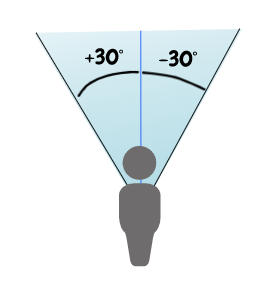
\includegraphics[width=0.3\textwidth]{images/degree_orientation.png}
    \caption{Η κατεύθυνση του χρήστη πρέπει να είναι μέσα σε ένα τόξο 60\degree για να θεωρείται έγκυρη. Αλλιώς παρέχεται κατάλληλη ανάδραση για αριστερή ή δεξιά στροφή.}
    \label{fig:degree-orientation}
\end{figure}
\begin{figure}[H]
    \centering
    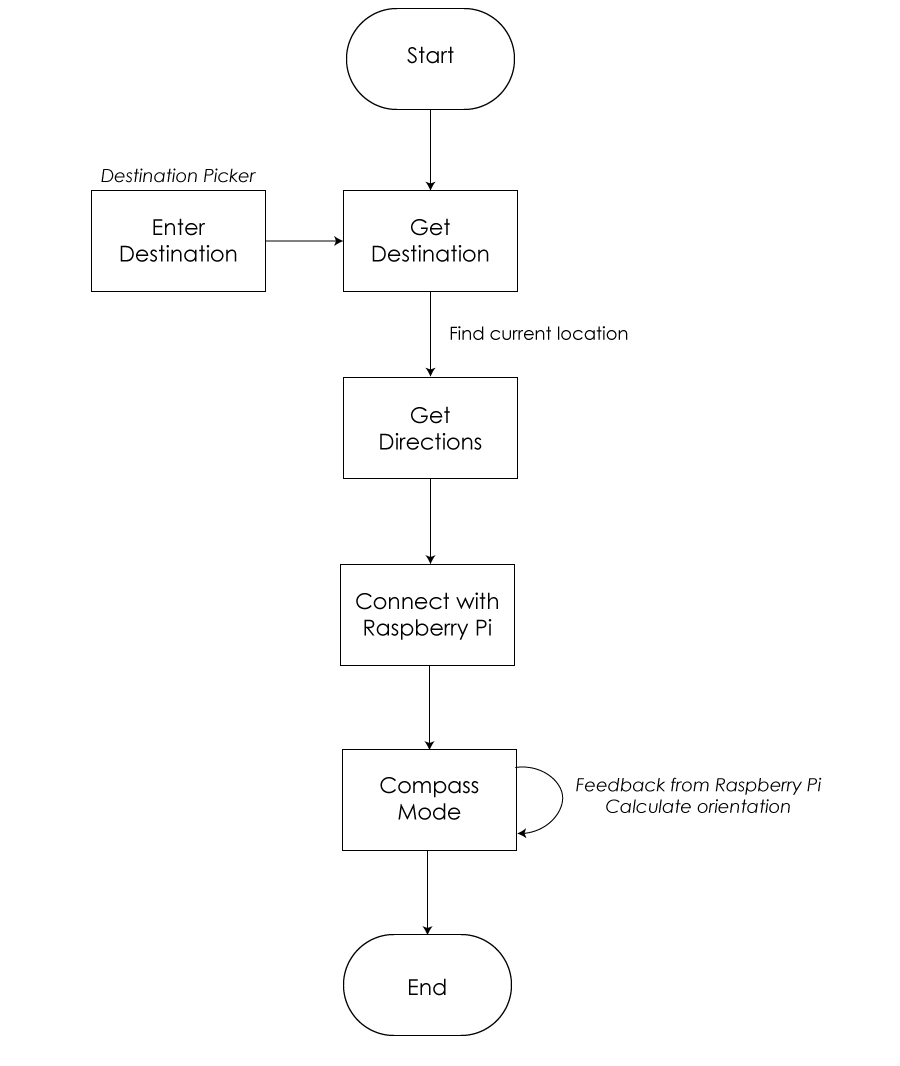
\includegraphics[width=0.8\textwidth]{images/working_diagram.png}
    \caption{Διάγραμμα ροής της Android εφαρμογής}
    \label{fig:working-diagram}
\end{figure}

\subsubsection{Προδιαγραφές εφαρμογής – Ελάχιστες απαιτήσεις}
Κατά την ανάπτυξη της εφαρμογής προέκυψαν διάφορες ανάγκες όσον αφορά την χρήση της από άτομα με προβλήματα όρασης. Βασικός μας στόχος ήταν να είναι όσο πιο απλή γίνεται με έμφαση στη λειτουργικότητα. Μια τέτοια εφαρμογή πρέπει:
\begin{enumerate}
    \item Να χαρακτηρίζεται από την απλότητα στη διεπιφάνεια χρήστη
    \item Να είναι διαισθητική, δηλαδή να είναι αυτονόητο αυτό που προσφέρει μην απαιτείται πολύς χρόνος εκπαίδευσης σε νέους χρήστες
    \item Να χρησιμοποιεί τεχνολογία πρόσβασης για άτομα με μειωμένη όραση, όπως χρήση δονήσεων, μετατροπή λόγου σε κείμενο και αντίστροφα.
\end{enumerate}

Από τις παραπάνω απαιτήσεις, στα πλαίσια της παρούσας εργασίας καταφέραμε να υλοποιήσουμε το 1, 2 και, εν μέρει, το 3. Λόγω περιορισμένου χρόνου δεν υλοποιήθηκε η μετατροπή από προφορικό λόγο σε κείμενο.
\newpage
\subsubsection{UX-UI Design}
Παρακάτω παρουσιάζονται μερικά στιγμιότυπα από τα διάφορα screens της εφαρμογής.
\begin{figure}[H]
    \centering
    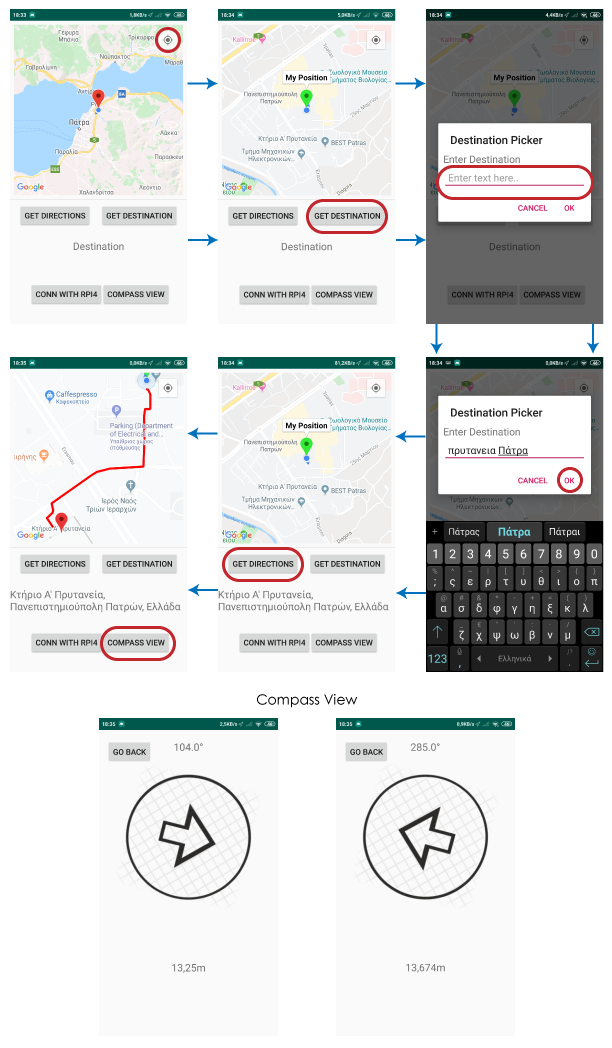
\includegraphics[width=0.7\textwidth]{images/ui_app.png}
    \caption{Διεπιφάνεια επαφής χρήστη}
    \label{fig:ui-app}
\end{figure}

Στο σχήμα \ref{fig:ui-app} παρουσιάζονται με κόκκινο πλαίσιο οι βασικοί τρόποι με τους οποίους αλληλεπιδρά ο χρήστης με το σύστημα. Η βασική ιδέα είναι ότι ο χρήστης, αφού εισάγει τον προορισμό του, θα τοποθετήσει το κινητό στη τσέπη του (ή θα το κρατάει στο χέρι του) και αυτό θα τον καθοδηγεί καθ' όλη την διάρκεια της πλοήγησης, μειώνοντας στο ελάχιστο την αλληλεπίδραση του χρήστη με το σύστημα. Η εφαρμογή εντοπίζει αυτόματα τον προσανατολισμό του χρήστη με τη βοήθεια των αισθητήρων επιταχυνσιομέτρου, γυροσκοπίου και πυξίδας. Είναι γεγονός ότι ο χρήστης που έχει προβλήματα όρασης θα εισάγει τον προορισμό του μέσω ενός συστήματος αναγνώρισης και μετατροπής ομιλίας σε κείμενο. Δυστυχώς, λόγω έλλειψης χρόνου δεν υλοποιήθηκε το συγκεκριμένο χαρακτηριστικό στα πλαίσια της παρούσας διπλωματικής εργασίας.

\subsection{Συσκευή απτικής ανατροφοδότησης – Haptic Device}
\subsubsection{Υπάρχουσες συσκευές απτικής ανατροφοδότησης}
Ως συσκευές απτικής ανατροφοδότησης μπορούν να χαρακτηριστούν όλες εκείνες οι συσκευές που παρέχουν κάποιου είδους πίεση στο δέρμα του χρήστη, π.χ. μέσω δόνησης. Την τελευταία δεκαετία έχουν εμφανιστεί πολλές τέτοιες συσκευές που είναι πολλά υποσχόμενες για την αλληλεπίδραση ανθρώπου-μηχανής. Μια πολύ ενδιαφέρουσα εναλλακτική που εξετάστηκε στα πλαίσια της διπλωματικής είναι το βραχιόλι Myo Armband \cite{MyoGestu49:online}, το οποίο τοποθετείται κάτω από τον αγκώνα και αποτελείται από πολλαπλούς αισθητήρες που διαβάζουν ηλεκτρομυογραφικά σήματα τα οποία ερμηνεύονται ως συγκεκριμένες κινήσεις. Αν και το Myo Armband παρέχει τη δυνατότητα δόνησης στο χέρι του χρήστη, δεν επιλέχθηκε τελικά λόγω του ότι η εταιρεία που το είχε έκλεισε και δεν υπήρχε η απαραίτητη υποστήριξη από την κοινότητα. Επιπλέον, η χρησιμοποίηση της συγκεκριμένης συσκευής θα πρόσθετε ακόμα ένα βάρος στον χρήστη, κάτι που εναντιώνεται στο κριτήριο της απλότητας και της παρεμβατικότητας που αναφέραμε νωρίτερα.

\begin{figure}[H]
    \centering
    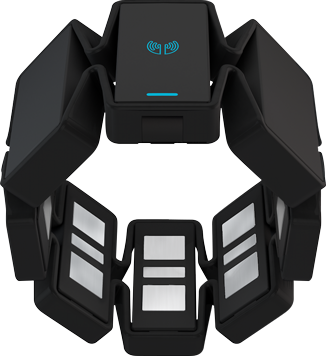
\includegraphics[width=0.6\textwidth]{images/myo_image_black.png}
    \caption{Myo Armband}
    \label{fig:myo}
\end{figure}

\subsubsection{Smartphone}
Μετά από εξέταση όλων των εναλλακτικών, καταλήξαμε στην επιλογή του smartphone ως το μέσο διάδοσης της απτικής ανάδρασης στο χρήστη. Αρχικά, η επιλογή αυτή μας εξυπηρετεί επειδή δεν απαιτείται η ένταξη μιας άλλης συσκευής στο σύστημα, η οποία πιθανόν να είχε προβλήματα συμβατότητας με τα υπόλοιπα μέρη. Επίσης, ο χρήστης δεν επιβαρύνεται με περιττά αντικείμενα, που θα δυσκόλευαν την εξωτερική του μετακίνηση και την εικόνα του προς τον υπόλοιπο κόσμο. Τέλος, το smartphone συνδέεται με το υπόλοιπο σύστημα και λαμβάνει κατάλληλα σήματα σχετικά με τον εντοπισμό και την αναγνώριση διαβάσεων και φαναριών. Ανάλογα το είδος του σήματος που φτάνει στο smartphone, αυτό με τη σειρά του παρέχει το κατάλληλο μοτίβο δόνησης στον χρήστη. Στα πλαίσια της παρούσας διπλωματικής εργασίας χρησιμοποιήθηκε το μοντέλο \emph{Redmi Note 4X}.

\section{Αλγόριθμοι πλοήγησης \& Λογισμικό (Software)}
Στην ενότητα αυτή παρουσιάζονται οι αλγόριθμοι που χρησιμοποιήθηκαν για την υλοποίηση του συστήματος πλοήγησης, καθώς και το λογισμικό που αξιοποιήθηκε για την ανάπτυξή του. Λαμβάνοντας υπόψιν το εύρος της υλοποίησης, ήταν αναγκαίος ο συνδυασμός πολλών διαφορετικών γνώσεων και εργαλείων, γεγονός που πολλές φορές δυσκόλεψε την υλοποίηση λόγω μη συμβατότητας. Παρόλα αυτά, η ενασχόληση του συγγραφέα της εργασίας με τόσα διαφορετικά εργαλεία και γλώσσες προγραμματισμού τον βοήθησε να αποκτήσει μια πιο ολοκληρωμένη άποψη για το συγκεκριμένο ερευνητικό πεδίο και να αναπτύξει πολλές νέες δεξιότητες.

\subsection{Χρησιμοποιηθέντα εργαλεία και γλώσσες προγραμματισμού}
Για την ανάπτυξη της εφαρμογής πλοήγησης σε λειτουργικό Android, επιλέχθηκε το λογισμικό της Google, Android Studio, το οποίο υποστηρίζει συγγραφή κώδικα σε Java, ενώ για την συγγραφή του κώδικα που αφορά τους αλγορίθμους επεξεργασίας εικόνας χρησιμοποιήθηκε το Visual Studio της Microsoft και η συγγραφή έγινε στη γλώσσα C++. Καθ' όλη την υλοποίηση των αλγορίθμων έγινε εκτεταμένη χρήση της γνωστής βιβλιοθήκης OpenCV (Open Computer Vision) και του Intel® RealSense™ SDK (Sofware Development Kit) που παρέχεται από την Intel.

\subsubsection{Android Studio - Java}
Το Android Studio IDE (Intergrated Development Environment) \cite{android_studio:online} είναι ίσως το πιο διαδεδομένο λογισμικό ανάπτυξης εφαρμογών για Android κινητά. Υποστηρίζεται επίσημα από την Google και μπορεί να εγκατασταθεί στις περισσότερες συσκευές (Windows, Mac, Linux). Το λογισμικό αυτό διευκολύνει τον σχεδιασμό του γραφικού περιβάλλοντος της εφαρμογής, δηλαδή της διεπιφάνειας χρήστη, και παρέχει τη δυνατότητα αξιοποίησης όλων των διαθέσιμων υπηρεσιών σε ένα smartphone, π.χ. GPS, IMU sensors, Bluetooth κ.α. Παράλληλα, ένα μεγάλο πλεονέκτημα του Android Studio είναι ότι επιτρέπει το γρήγορο και άμεσο testing της εφαρμογής υπό ανάπτυξη στο κινητό του χρήστη, ή σε κάποιον προσομοιωτή (emulator).

Πιο συγκεκριμένα, χρησιμοποιήθηκε η έκδοση \emph{Android Studio 3.5.1}, η οποία παρέχει την δυνατότητα συγγραφής κώδικα σε Java \cite{wiki:java} και σε Kotlin \cite{wiki:kotlin}, η οποία είναι μια παραλλαγή της Java. Όπως προαναφέρθηκε, επιλέχθηκε η ανάπτυξη σε Java, λόγω της μεγαλύτερης και ευρύτερης υποστήριξης από την κοινότητα.

\begin{figure}[H]
    \centering
    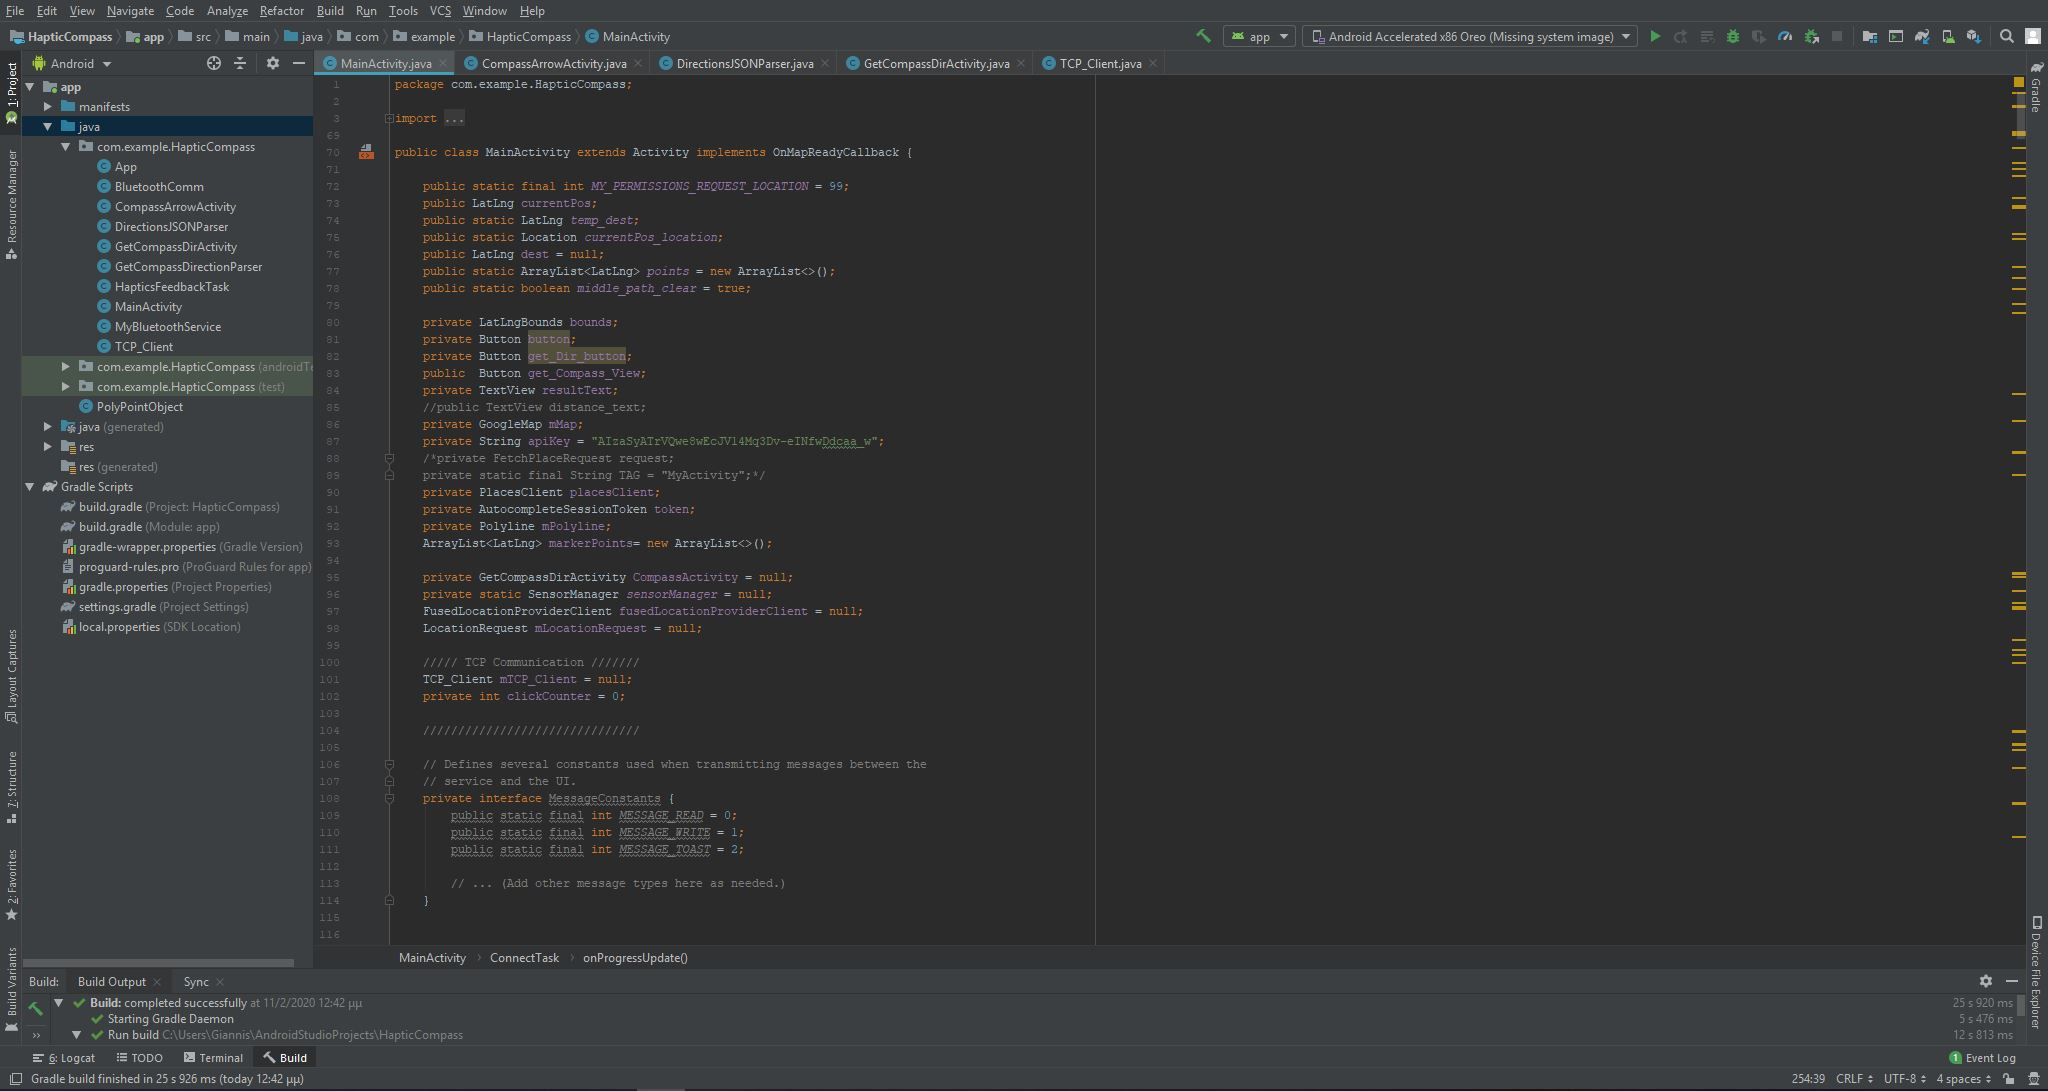
\includegraphics[width=\textwidth]{images/android_studio.JPG}
    \caption{Προγραμματιστικό περιβάλλον Android Studio IDE}
    \label{fig:android-studio}
\end{figure}

\subsubsection{Visual Studio - C++}
Η κύρια ανάπτυξη κώδικα έγινε σε C++ στο περιβάλλον του\emph{ Visual Studio 2017 IDE} \cite{VisualSt72:online}. Πρόκειται για ένα από τα καλύτερα IDE, που προσφέρουν αρκετές διευκολύνσεις κατά την ανάπτυξη κώδικα, όπως είναι η αυτόματη συμπλήρωση, εντοπισμός σφαλμάτων, debugging κ.α. Ένα IDE (Intergrated Development Environment), ή αλλιώς ολοκληρωμένο περιβάλλον ανάπτυξης, είναι μια σουίτα λογισμικού που βοηθάει στην ανάπτυξη προγραμμάτων υπολογιστή και περιλαμβάνει κάποιον επεξεργαστή πηγαίου κώδικα, έναν μεταγλωττιστή, εργαλεία αυτόματης παραγωγής κώδικα, debugger, linker, version control systems (git) και εργαλεία κατασκευής γραφικών διασυνδέσεων χρήστη.

Ως εναλλακτική επιλογή υπήρχε η ανάπτυξη του κώδικα στη γλώσσα Python \cite{wiki:python}, η οποία είναι πολύ διαδεδομένη τα τελευταία χρόνια και υποστηρίζεται σε πολύ μεγάλο βαθμό από την κοινότητα, ωστόσο απορρίφθηκε επειδή στόχος της διπλωματικής ήταν η υλοποίηση κώδικα για embedded συστήματα, όπως το Raspberry Pi, για τα οποία η C++ είναι πιο κατάλληλη γλώσσα. Επίσης, η Python είναι εν γένει πιο αργή σε σύγκριση με την C++, καθώς η πρώτη ακολουθεί μια διαδικασία "μετάφρασης", ενώ η δεύτερη γίνεται compile κατευθείαν σε γλώσσα μηχανής. Τέλος, ο κώδικας που γράφτηκε στο Visual Studio μεταφέρθηκε στο Raspberry Pi αυτούσιος, με μικρές μόνο τροποποιήσεις, ώστε να είναι συμβατός με το λειτουργικό σύστημα Linux του Raspberry Pi.

\begin{figure}[H]
    \centering
    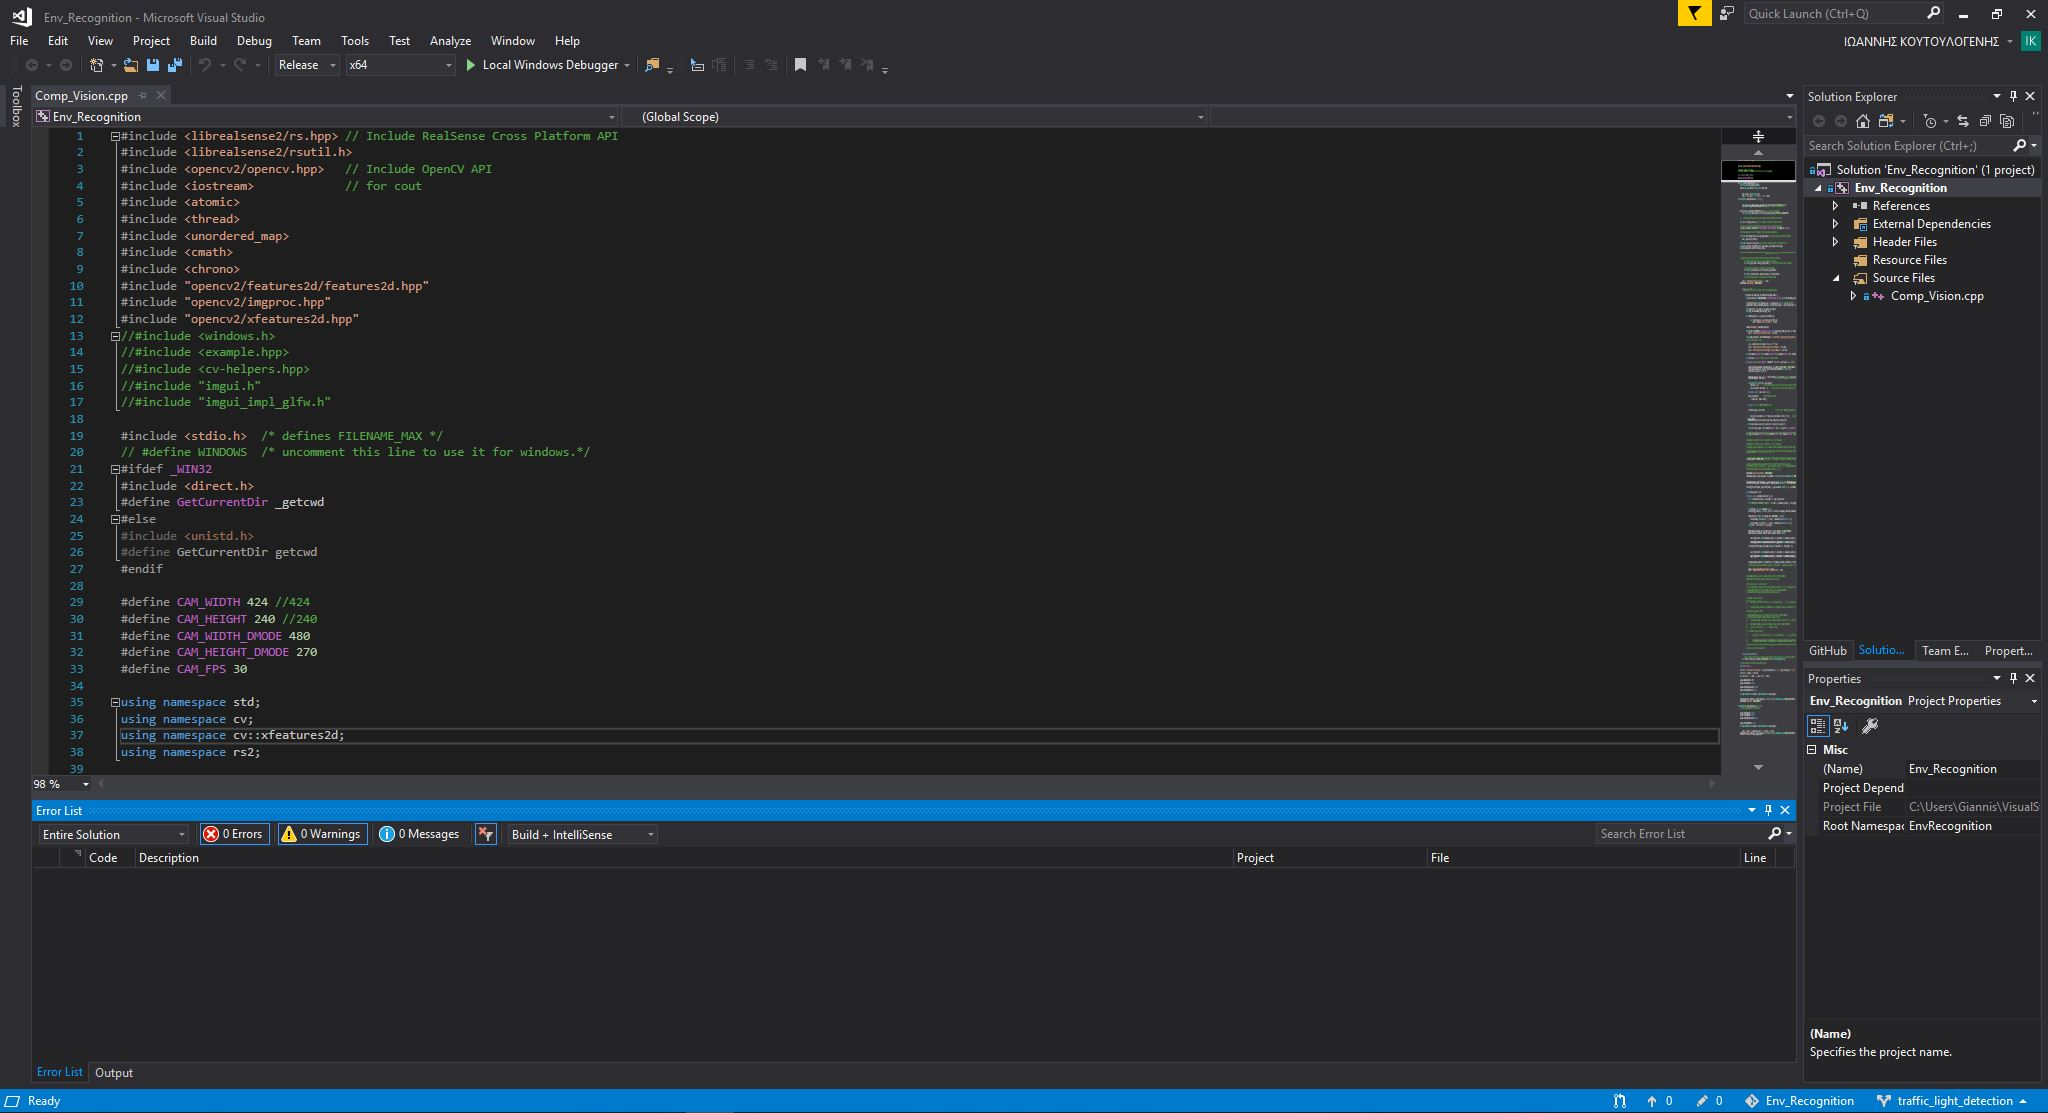
\includegraphics[width=\textwidth]{images/vs17.JPG}
    \caption{Προγραμματιστικό περιβάλλον Visual Studio IDE}
    \label{fig:visual-studio}
\end{figure}

\subsubsection{OpenCV}
Στα πλαίσια της διπλωματικής χρησιμοποιήθηκε η έκδοση \emph{OpenCV 4.2.0}. Η βιβλιοθήκη OpenCV \cite{OpenCVWi26:online} είναι μια συλλογή από βελτιστοποιημένες συναρτήσεις που χρησιμοποιούνται κυρίως στο πεδίο της μηχανικής όρασης, ενώ παράλληλα παρουσιάζει συμβατότητα με τις περισσότερες πλατφόρμες και χρησιμοποιείται κάτω από την άδεια ανοιχτού κώδικα. Ο λόγος που επιλέχθηκε η αξιοποίηση της OpenCV είναι η ενσωμάτωση πολλών έτοιμων φίλτρων και συναρτήσεων για επεξεργασία εικόνας, που είναι ήδη βελτιστοποιημένες για πιο αποδοτική χρήση, επιτρέποντας στον προγραμματιστή να ασχοληθεί με πιο αφηρημένες έννοιες όσον αφορά τον σχεδιασμό του συστήματος. Τέλος, η υποστήριξη της OpenCV από την κοινότητα είναι καθολική και είναι πολύ πιο εύκολο να διορθωθούν τυχόν σφάλματα στον κώδικα. Η κύρια γλώσσα προγραμματισμού καθώς και η γλώσσα στην οποία είναι γραμμένη η OpenCV είναι η C++.

\begin{figure}[H]
    \centering
    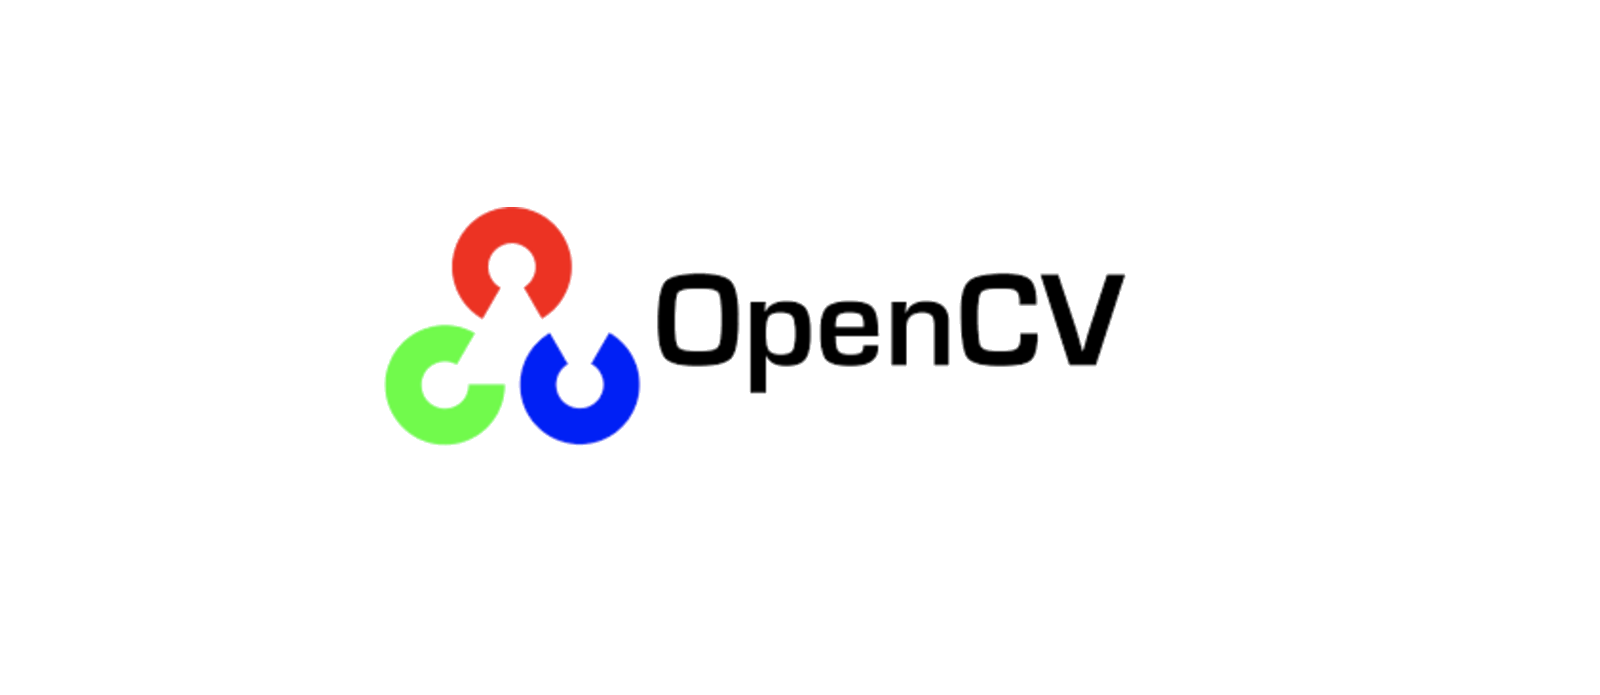
\includegraphics[width=\textwidth]{images/opencv.png}
    \caption{Λογότυπο βιλβιοθήκης OpenCV}
    \label{fig:opencv}
\end{figure}

\subsubsection{Intel® RealSense™ SDK 2.0}
Παράλληλα με την OpenCV αξιοποιήθηκε και η βιβλιοθήκη LibRealsense \cite{IntelRea94:online} που παρέχετε από το SDK της κάμερας Intel Realsense. Πιο συγκεκριμένα, η κάμερα που χρησιμοποιήθηκε έρχεται μαζί με ένα πακέτο συναρτήσεων που υλοποιούν βασικά κομμάτια επικοινωνίας της κάμερας με το πρόγραμμα και διευκολύνουν την πρόσβαση στα δεδομένα της κάμερας, π.χ. depth maps και rgb frames. Παράλληλα, μέσα από το συγκεκριμένο SDK δίνεται η δυνατότητα παρέμβασης στις εσωτερικές προεπιλεγμένες ρυθμίσεις της κάμερας και παρέχονται βασικά παραδείγματα και χρήσιμα εργαλεία αποσφαλμάτωσης (debugging).

\begin{figure}[H]
    \centering
    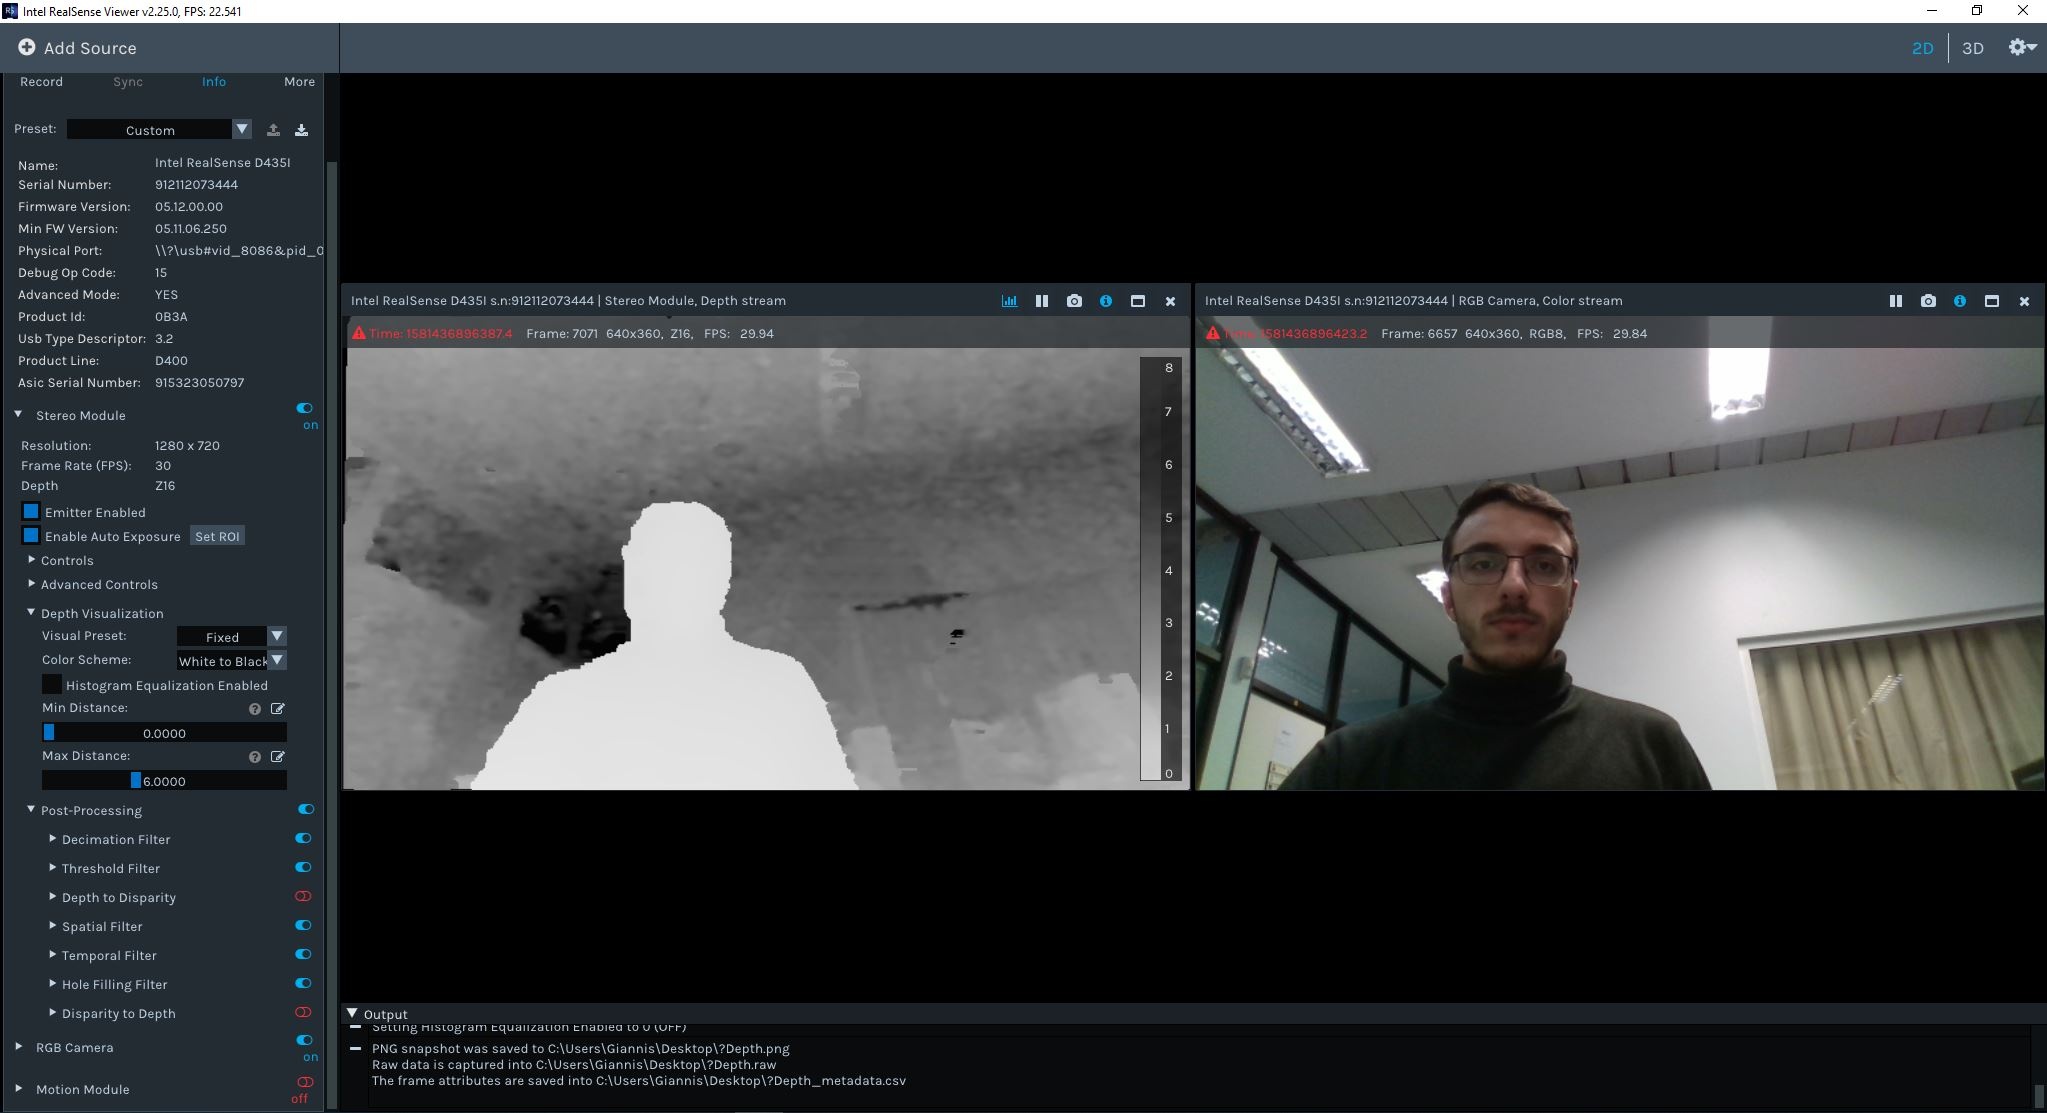
\includegraphics[width=\textwidth]{images/realsense_viewer.JPG}
    \caption{RealSense Viewer από το RealSense™ SDK 2.0}
    \label{fig:librealsense}
\end{figure}

\subsubsection{Raspberry Pi - Linux OS}
Το λειτουργικό που χρησιμοποιήθηκε στο Raspberry Pi 4 είναι το \emph{Ubuntu Server 19.10} 64-bit \cite{InstallU96:online}, με κωδική ονομασία Eoan Ermine, το οποίο υποστηρίζει πλήρως τις δυνατότητες του RPi4. Επειδή το λειτουργικό σύστημα Ubuntu Server δεν έχει ενσωματωμένο γραφικό περιβάλλον, εγκαταστάθηκε το MATE Desktop Environment \cite{MATEDesk37:online}.

\begin{figure}[H]
    \centering
    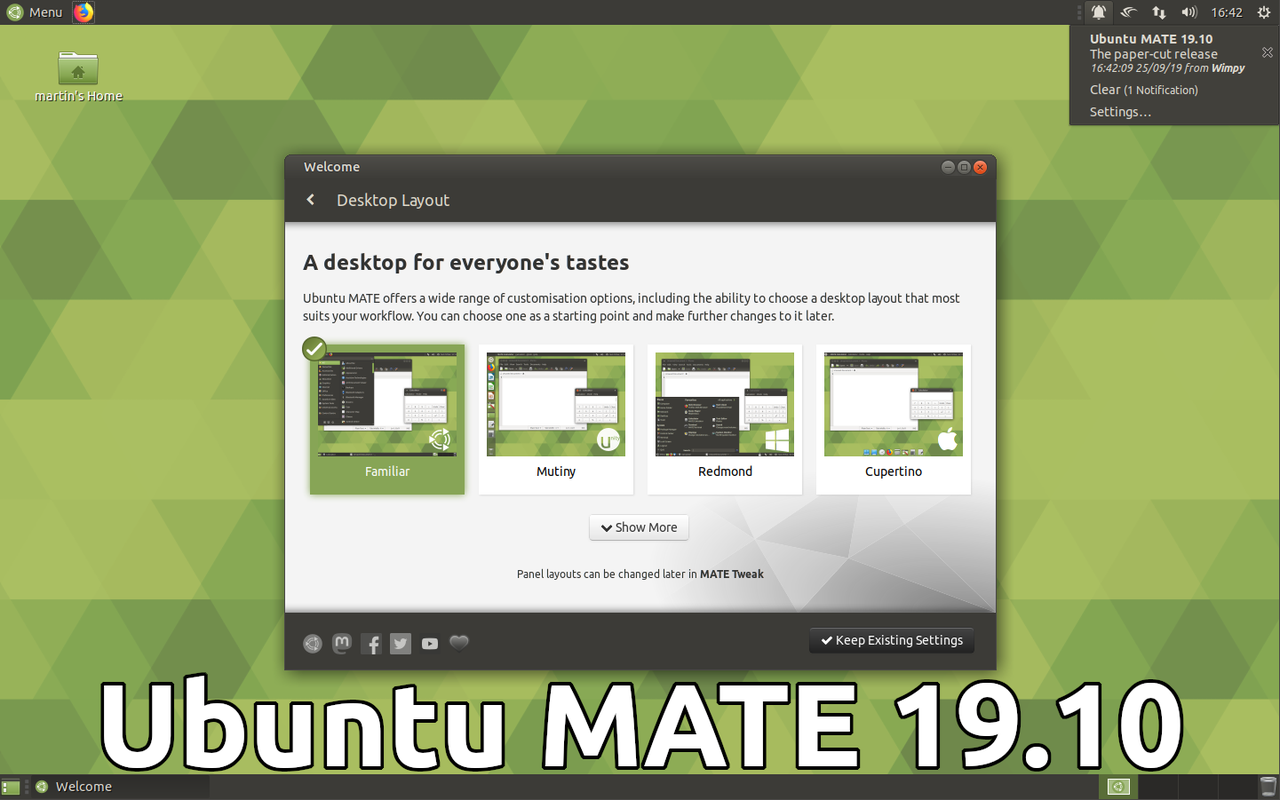
\includegraphics[width=\textwidth]{images/eoan-ermine-desktop.png}
    \caption{Ubuntu 19.10 with MATE Desktop Environment}
    \label{fig:mate}
\end{figure}

\subsection{Αλγόριθμοι επεξεργασίας εικόνας σε πραγματικό χρόνο}
Παρακάτω αναλύονται οι αλγόριθμοι που χρησιμοποιήθηκαν στην παρούσα διπλωματική εργασία, αποφεύγοντας όσο γίνεται τις πολύ τεχνικές λεπτομέρειες που αφορούν την προγραμματιστική υλοποίησή τους. Αρχικά, είναι σημαντικό να αναφέρουμε ότι το πρόγραμμά μας αποτελείται από δύο διαφορετικά threads, δηλαδή κομμάτια κώδικα που τρέχουν το ένα ανεξάρτητα από το άλλο, όπου το πρώτο thread (εφεξής \emph{processing thread}) τρέχει στο παρασκήνιο και είναι υπεύθυνο για να "παραλαμβάνει" τα frames από την κάμερα και να εφαρμόζει ένα αρχικό φιλτράρισμα μόνο στα depth frames, ενώ στο δεύτερο thread (εφεξής \emph{main thread}) γίνεται η κυρίως επεξεργασία και ανάλυση των εικόνων και τρέχει σε ένα συνεχή βρόχο για όσο είναι ανοιχτό το πρόγραμμα. Ο λόγος που χρησιμοποιούμε δύο διαφορετικά thread είναι για να αποφύγουμε καταστάσεις όπου το πρόγραμμα "κολλάει" αναμένοντας κάποιο frame να φτάσει από την κάμερα.

\begin{figure}[H]
    \centering
    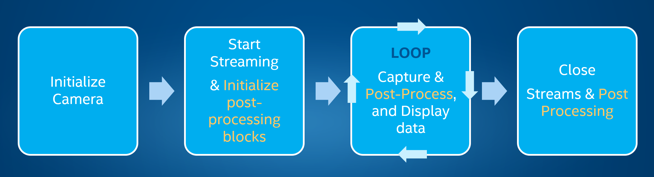
\includegraphics[width=0.8\textwidth]{images/frames_flow.png}
    \caption{Διάγραμμα ροής ενός frame}
    \label{fig:frame-flow}
\end{figure}

Το πρόγραμμα ρυθμίζεται να λειτουργεί με RGB frames ανάλυσης 424x240 στα 30fps και Depth frames ανάλυσης 480x270 στα 30fps. Οι συγκεκριμένες αναλύσεις επιλέχθηκαν ώστε να κάνει την επεξεργασία πιο γρήγορη, μιας και δεν είναι αναγκαία μεγαλύτερη ενάλυση για την εφαρμογή που θέλουμε. Στη συνέχεια, αφού παραληφθεί κάποιο depth frame στο processing thread, εφαρμόζονται τα εξής φίλτρα με σειρά προτεραιότητας \cite{DepthPos51:online}:
\begin{enumerate}
    \item \textbf{Decimation filter}: Φίλτρο που μειώνει την πολυπλοκότητα της εικόνας, εφαρμόζοντας ουσιαστικά υπο-δειγματοληψία (downsampling) της αρχικής εικόνας. Πιο συγκεκριμένα, εφαρμόζεται συνέλιξη του αρχικού frame με ένα πίνακα kernel 2x2, χρησιμοποιώντας την μέση τιμή των pixel που καλύπτονται από τον kernel. Αντίστοιχα, το μέγεθος της εικόνας μειώνεται αναλογικά και στις δύο διαστάσεις για να διατηρηθεί η αρχική αναλογία διαστάσεων. Η διαδικασία αυτή μπορεί να αυξήσει την ταχύτητα της μετέπειτα επεξεργασίας μέχρι 4 φορές, ενώ παράλληλα συμβάλλει στην εξάλειψη τυχόν κενών pixels (black holes).
    \item \textbf{Spatial Edge-Preserving filter}: Φίλτρο που εξομαλύνει τον θόρυβο βάθους (depth noise), διατηρεί τις γωνίες/άκρες και κάνει τις επιφάνειες πιο επίπεδες \cite{GastalOliveira2011DomainTransform}.
    \begin{figure}[H]
        \centering
        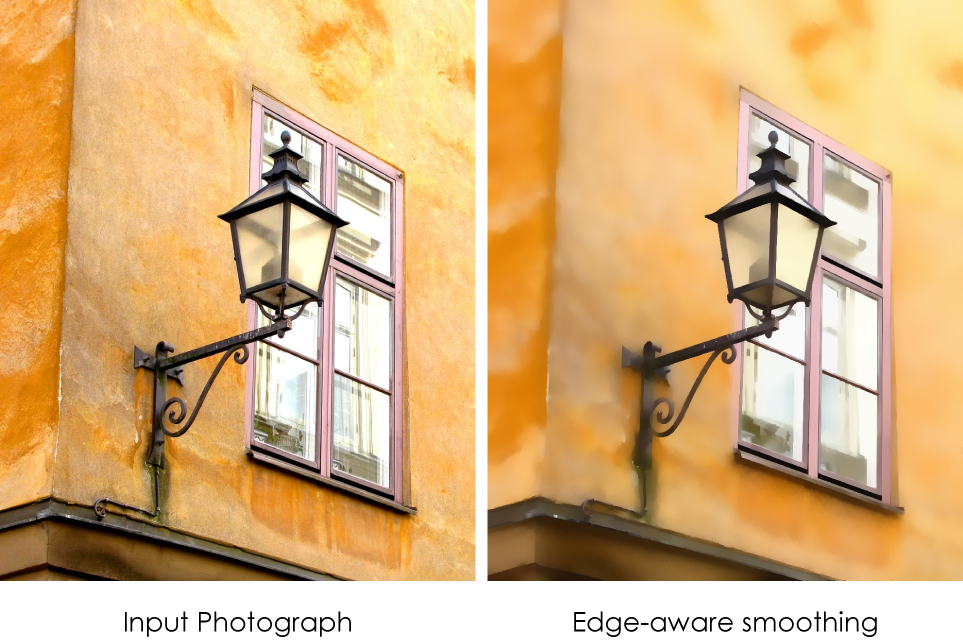
\includegraphics[width=0.8\textwidth]{images/edge_preserving_example.png}
        \caption{Παράδειγμα εφαρμογής του Spatial Filter βασιζόμενο στο \cite{GastalOliveira2011DomainTransform}}
        \label{fig:spatial-example}
    \end{figure}

    \item \textbf{Temporal filter}: Φίλτρο που βελτιώνει τα δεδομένα βάθους με βάση τα αντίστοιχα frames σε προηγούμενη χρονική περίοδο. Πιο συγκεκριμένα, για κάθε pixel που είναι κενό ή έχει λανθασμένη τιμή κοιτάζει το ιστορικό και χρησιμοποιεί την τιμή που είχε το pixel αυτό σε προηγούμενο frame. Ο κανόνας που χρησιμοποιείται είναι ότι η τιμή ενός κενού pixel αντικαθίσταται από την τελευταία έγκυρη τιμή, αν αυτή είναι έγκυρη στα τελευταία 2 από τα 4 frames.
    \item \textbf{Hole-Filling filter}: Φίλτρο που χρησιμοποιείται για εξάλειψη τυχόν εναπομείναντων κενών pixels (holes). Το φίλτρο κάνει αναζήτηση σε μια γειτονιά ενός pixel και η διαδικασία που ακολουθείται είναι ότι κάθε κενό pixel αντικαθίσταται από την τιμή του γειτονικού pixel με την κοντινότερη απόσταση από τον αισθητήρα (nearest from around).
    \begin{figure}[H]
        \centering
        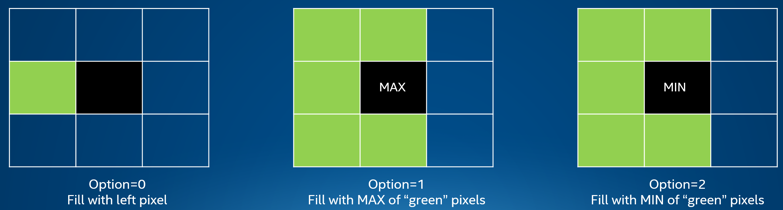
\includegraphics[width=0.8\textwidth]{images/hole_filling.png}
        \caption{Επιλογές φίλτρου εξάλειψης κενών pixels (hole filling)}
        \label{fig:hole-filling}
    \end{figure}
\end{enumerate}

Στη συνέχεια, τα RGB και Depth frames προωθούνται στο main thread και ξεκινάει η εφαρμογή των αλγορίθμων που θα περιγραφεί παρακάτω.

\begin{figure}[H]
    \centering
    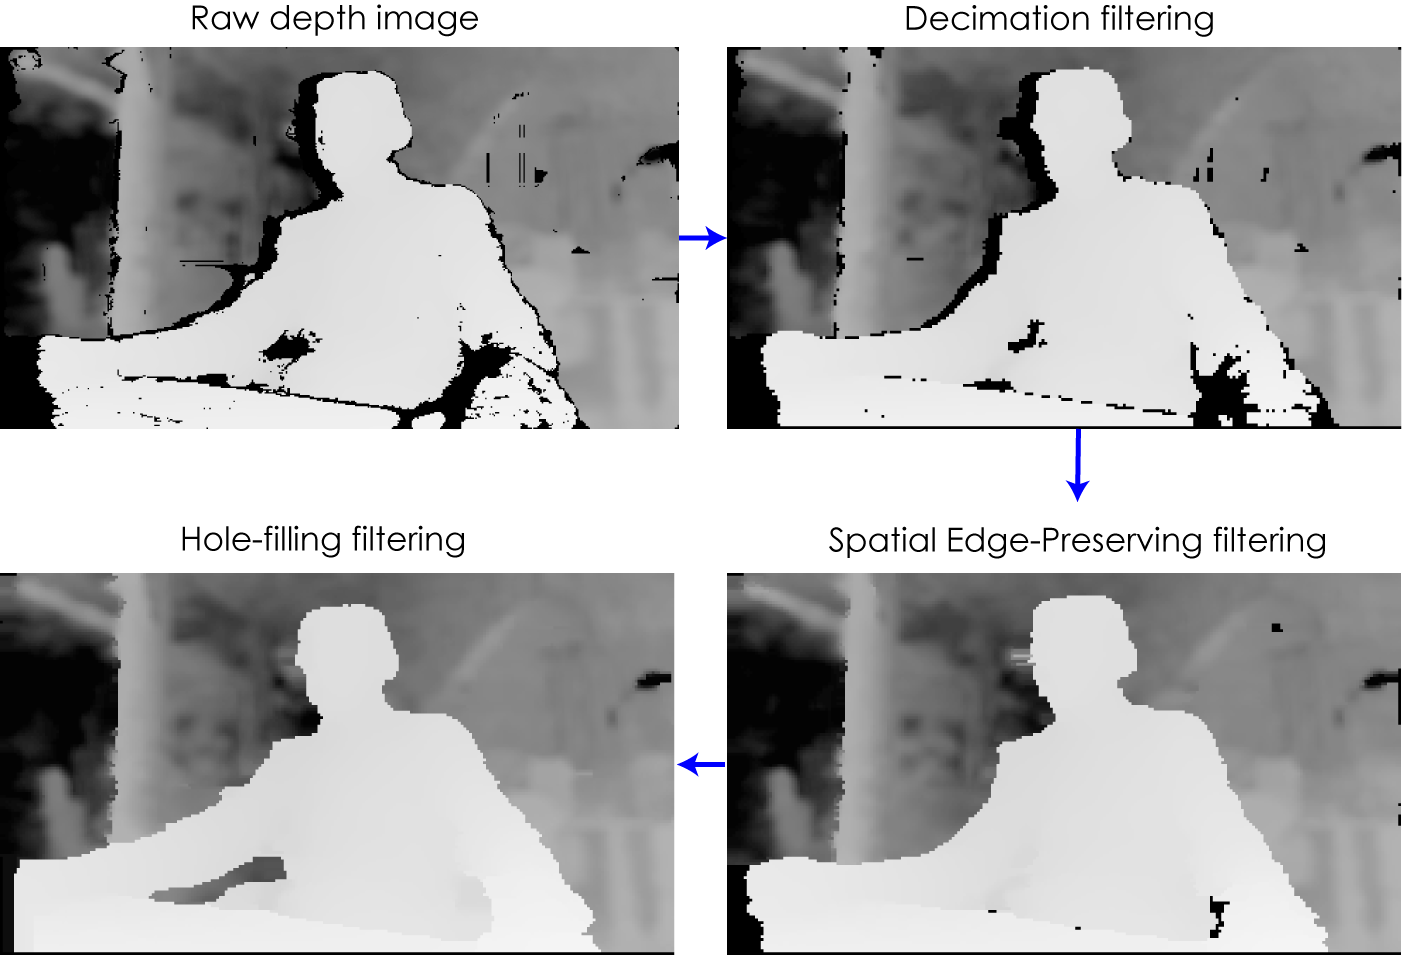
\includegraphics[width=0.8\textwidth]{images/preprocessing.png}
    \caption{Παράδειγμα εφαρμογής φίλτρων στο στάδιο του preprocessing (εξαιρείται το temporal filter, γιατί στην συγκεκριμένη λήψη δεν άλλαζε σημαντικά το αποτέλεσμα)}
    \label{fig:preprocessing}
\end{figure}

\subsubsection{Αναγνώριση διάβασης πεζών}
Η αναγνώριση διάβασης πεζών βασίζεται σε μια παραλλαγή του αλγορίθμου που προτείνεται από τους Wu, X., Hu, R., \& Bao, Y. (2019), στη δημοσίευση με τίτλο \emph{Block-Based Hough Transform for Recognition of Zebra Crossing in Natural Scene Images} \cite{wu_block-based_2019}. Βασική προϋπόθεση είναι να τρέχει σε πραγματικό χρόνο (real-time) και να παρέχει αξιόπιστα αποτελέσματα. Ο προτεινόμενος αλγόριθμος βασίζεται στην εφαρμογή του Μετασχηματισμού Hough σε συγκεκριμένα τμήματα της αρχικής εικόνας που καλούνται blocks και χωρίζεται σε δύο φάσεις:
\begin{enumerate}
    \item την φάση της αναγνώρισης ανά block (\nameref{block-based}), και
    \item την φάση της σύνθεσης (\nameref{synthesize}). 
\end{enumerate}

\paragraph{Χαρακτηριστικά και περιορισμοί διάβασης πεζών}
Η κλασσική διάβαση πεζών αποτελείται από λευκές και μαύρες λωρίδες που εναλλάσσονται μεταξύ τους και θυμίζουν το ασπρόμαυρο μοτίβο της ζέβρας (Σχήμα \ref{fig:zebra-crossing}). Το σύστημα πλοήγησης που παρουσιάζεται στη συγκεκριμένη εργασία θέτει ως βασική προϋπόθεση την ύπαρξη διάβασης πεζών τύπου ζέβρας, ώστε να μπορεί να βοηθήσει τον χρήστη να διασχίσει ένα δρόμο. Τέτοιου τύπου διαβάσεις χαρακτηρίζονται από τις 2 παρακάτω ιδιότητες:
\begin{itemize}
    \item Οι μεγάλες πλευρές των λωρίδων είναι παράλληλες
    \item Η χρωματική ένταση έχει διπολικά χαρακτηριστικά (άσπρο-μαύρο)
\end{itemize}
Ωστόσο, πολλές φορές οι παραπάνω ιδιότητες εκφυλίζονται όταν πρόκειται για διαβάσεις στο πραγματικό περιβάλλον, επειδή άλλοι παράγοντες (όπως συνθήκες φωτισμού, αντανακλάσεις, ξεθώριασμα, γεωμετρία δρόμου, οπτική παρεμπόδιση) επηρεάζουν σημαντικά το πως φαίνονται οι διαβάσεις.

\begin{figure}[H]
    \centering
    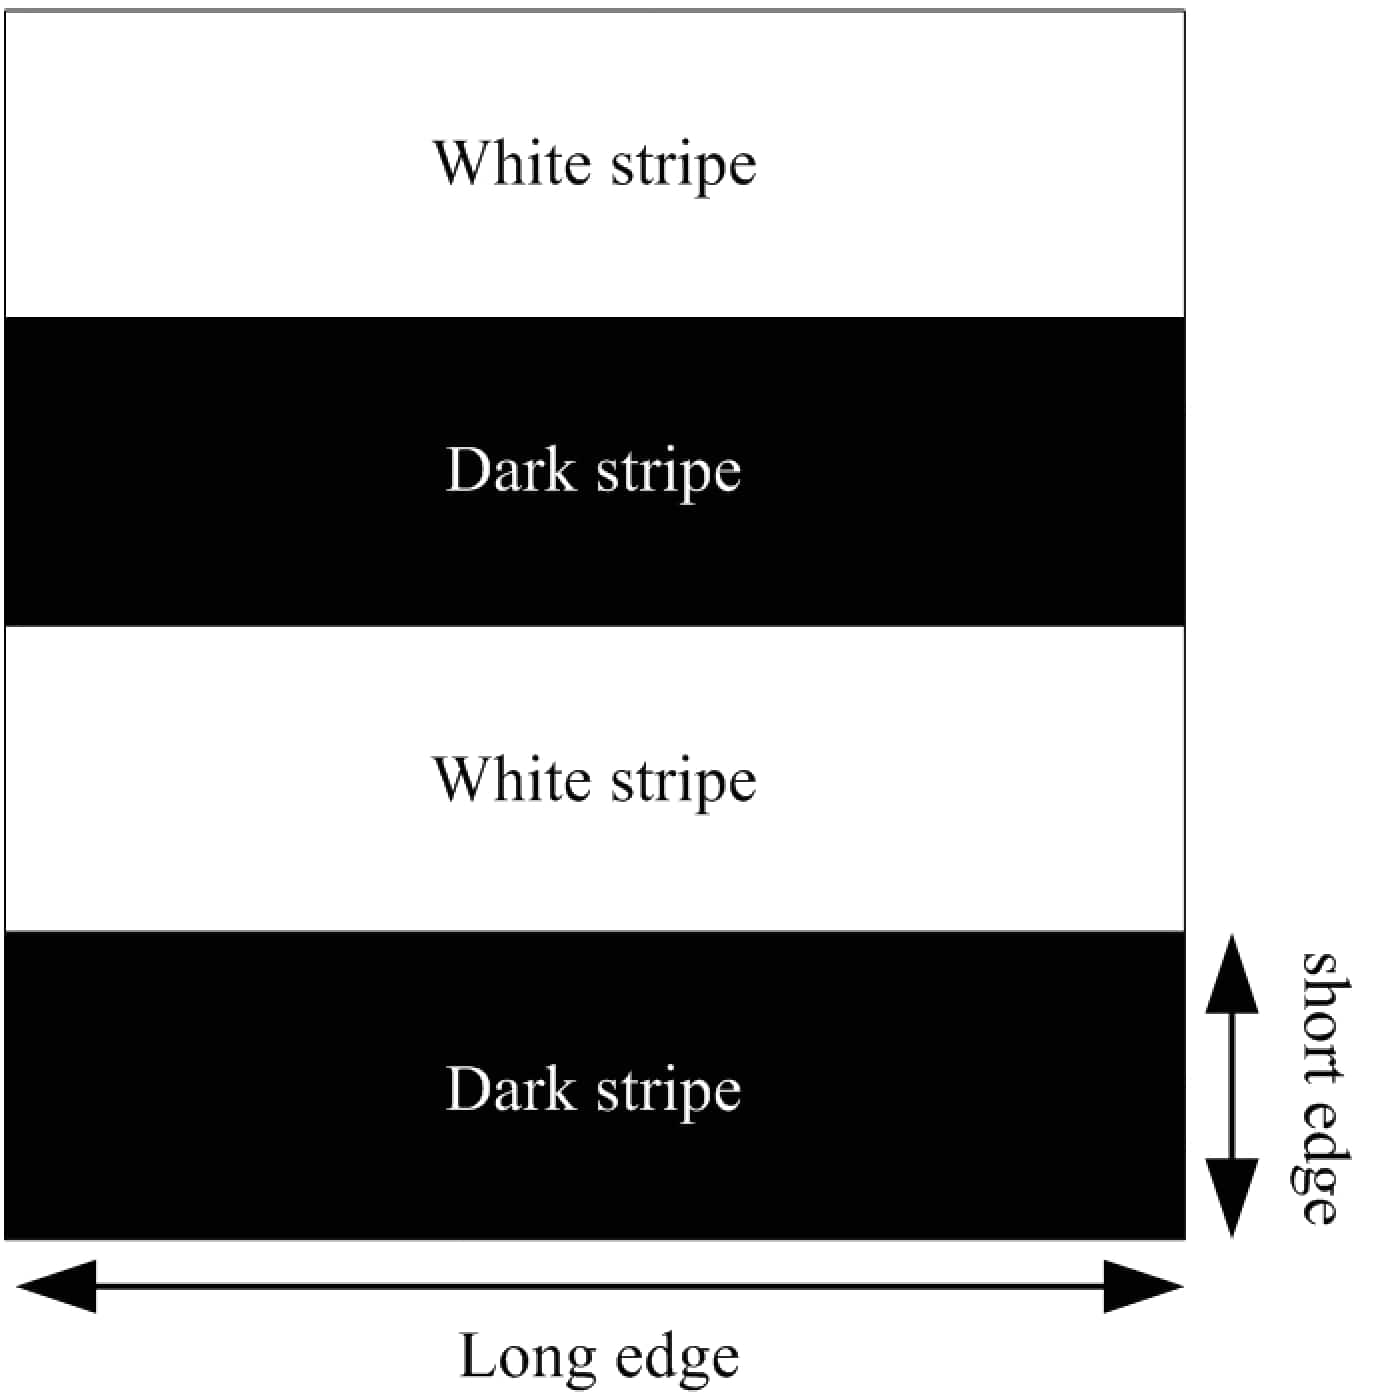
\includegraphics[width=0.5\textwidth]{images/zebra_crossing.jpg}
    \caption{Κλασσική μορφή διάβασης πεζών τύπου ζέβρας \cite{wu_block-based_2019}}
    \label{fig:zebra-crossing}
\end{figure}

\paragraph{Η προτεινόμενη μέθοδος}
Επειδή συνήθως οι διαβάσεις πεζών βρίσκονται στο κάτω μέρος της εικόνας όπως στέκεται ένας πεζός, καταρχήν περιορίζουμε την αρχική εικόνα ορίζοντας μια περιοχή ενδιαφέροντος, η οποία περιλαμβάνει το κάτω μισό της αρχικής εικόνας (50\% του ύψους) και το 80\% του αρχικού πλάτους. Έπειτα αυτή η περιοχή διαιρείται σε πολλαπλά επικαλυπτόμενα blocks που έχουν ίδιο ύψος με την περιοχή ενδιαφέροντος, αλλά μικρότερο πλάτος. Αφού οριστεί το μέγεθος κάθε block (στη παρούσα εργασία επιλέχθηκε το πλάτος κάθε block ίσο με το 1/3 του πλάτους της περιοχής ενδιαφέροντος), το πρόγραμμα μπαίνει σε έναν βρόχο όπου εφαρμόζεται ο Μετασχηματισμός Hough σε κάθε επιμέρους block. Όπως αναφέρθηκε, τα blocks είναι επικαλυπτόμενα, δηλαδή σε κάθε επανάληψη του βρόχου μπαίνει ένα νέο block το οποίο είναι μετατοπισμένο κατά μερικά pixels πιο δεξιά στον άξονα x σε σχέση με το προηγούμενο, μέχρι να φτάσουμε στο τέλος της περιοχής ενδιαφέροντος.
\begin{displayquote}
\emph{Ο αριθμός των pixels που μετατοπίζεται το block σε κάθε επανάληψη εξαρτάται από την επιλογή του χρήστη και επηρεάζει άμεσα την ποιότητα αλλά και την ταχύτητα του αλγορίθμου.}
\end{displayquote}
Όσο μικρότερη είναι η μετατόπιση του block τόσο πιο αναλυτικός γίνεται ο αλγόριθμος και παράγει καλύτερα αποτελέσματα, σε βάρος όμως της ταχύτητας. Αντίθετα, όσο μεγαλύτερη γίνεται η μετατόπιση τόσο πιο γρήγορος γίνεται ο αλγόριθμος με αντίστοιχη μείωση της ποιότητας του αποτελέσματος. Στη παρούσα εργασία, μετά από αρκετές δοκιμές, επιλέχθηκε εμπειρικά η μετατόπιση κατά 75 pixels σε κάθε επανάληψη, που αποτελεί έναν "καλό" συμβιβασμό ανάμεσα στην ποιότητα και την ταχύτητα.

Ο αλγόριθμος χρησιμοποιεί μια λογική όπου σε κάθε pixel ανατίθεται ένα σκορ, το οποίο στην αρχή είναι μηδέν. Εάν εντοπιστούν παράλληλες γραμμές σε ένα block, τότε εκτιμάται η γωνία τους και μεταβάλεται το σκορ των pixels που περιέχονται σε αυτό το block κατά μία συγκεκριμένη φόρμουλα που παρουσιάζεται παρακάτω:$$score[pixel] = 0.2\times score[pixel] + 0.8\times number\textunderscore of\textunderscore pixels\textunderscore in\textunderscore parallel\textunderscore lines$$ Παρατηρούμε ότι το σκορ ενός pixel του block εξαρτάται κατά 20\% από την προηγούμενη τιμή του και κατά 80\% από το πόσο ισχυρή είναι η παρουσία των παράλληλων γραμμών στο εκάστοτε block. Αφού η διαδικασία αυτή γίνει για κάθε block, στο τέλος υπολογίζεται ο μέσος όρος των γωνιών, ώστε να βρεθεί η κατεύθυνση της διάβασης, και τα αθροιστικά σκορ συνθέτονται για να βρεθεί η θέση της διάβασης στην εικόνα.

\begin{figure}[H]
    \centering
    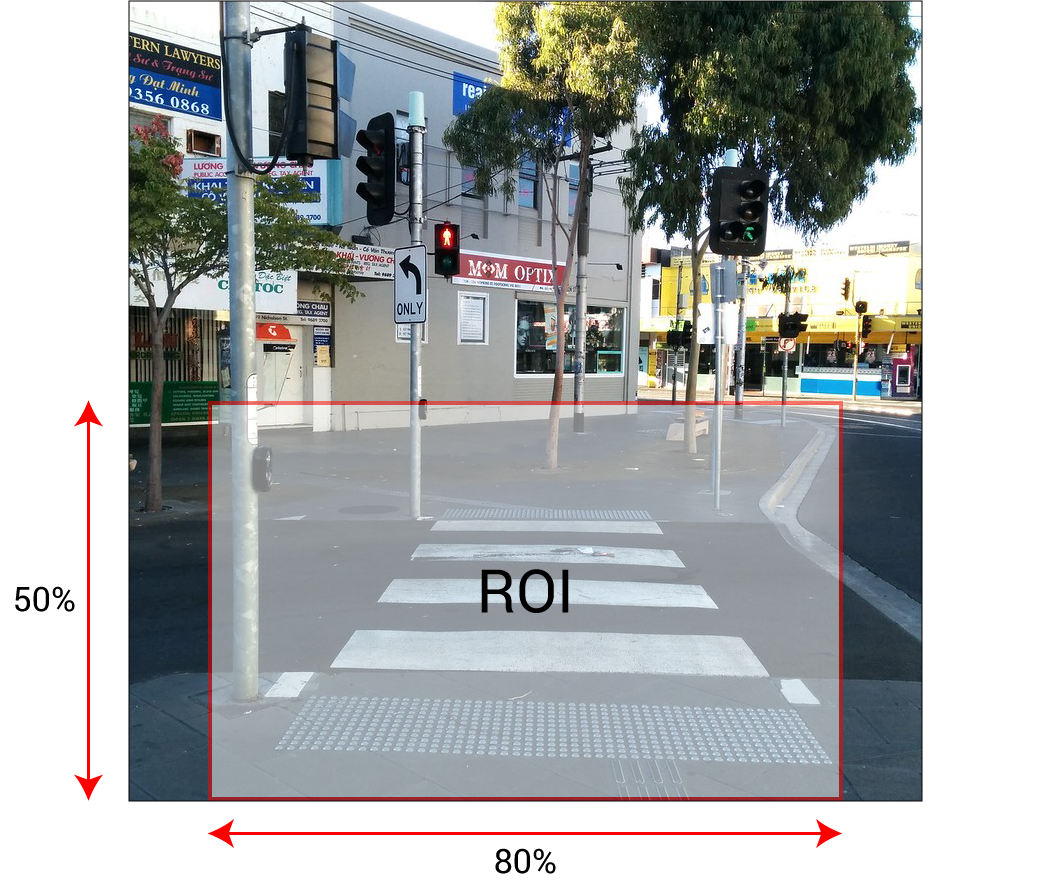
\includegraphics[width=0.6\textwidth]{images/lower_roi.png}
    \caption{Επιλογή περιοχής ενδιαφέροντος (ROI) για εντοπισμό διάβασης πεζών}
    \label{fig:lower-roi}
\end{figure}

\paragraph{Canny Edge Detector \& Hough Transform}
Στην υλοποίηση χρησιμοποιήθηκαν δύο πολύ διαδεδομένες τεχνικές στο χώρο της επεξεργασίας εικόνας, ο μετασχηματισμός Hough και το φίλτρο Canny:
\begin{itemize}
    \item \emph{Canny Edge Detector}: Το φίλτρο Canny αποτελεί μια από τις πιο γνωστές μεθόδους εξαγωγής των ακμών από μια εικόνα \cite{wiki:canny}. Ως ακμή ορίζεται το όριο μεταξύ περιοχών με σχετικά διακριτές τιμές χρωματικών πυκνοτήτων. Με τον όρο ακμές για μια ασπρόμαυρη εικόνα, αναφερόμαστε σε αλλαγές της φωτεινότητας μεταξύ γειτονικών περιοχών της. Τα βήματα του φίλτρου Canny είναι τα ακόλουθα:
    \begin{itemize}
        \item Βήμα 1: Εφαρμογή του γκαουσιανού φίλτρου (Gaussian Filtering) για εξομάλυνση της εικόνας και ελαχιστοποίηση της επίδρασης του θορύβου.
        \begin{figure}[H]
            \centering
            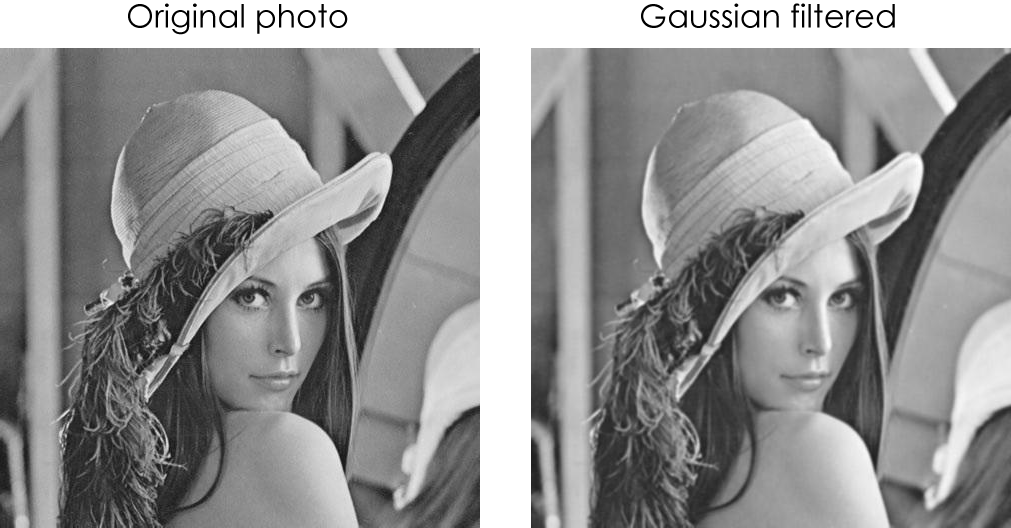
\includegraphics[width=0.8\textwidth]{images/gaussian_filtr.png}
            \caption{Εφαρμογή Gaussian Filter}
            \label{fig:gaussian}
        \end{figure}
        \item Βήμα 2: Εφαρμογή του τελεστή διαφόρισης στην εικόνα (συνέλιξη τελεστή με εικόνα Α) για να βρεθεί η κατευθυντική παράγωγος της εικόνας. Το φίλτρο Canny που υλοποιείται στην βιβλιοθήκη OpenCV χρησιμοποιεί τον τελεστή Sobel \cite{wiki:sobel}:
        \[ G_x = \begin{bmatrix}
            +1 & 0 & -1\\
            +2 & 0 & -2\\
            +1 & 0 & -1\\
        \end{bmatrix} * A, G_y = \begin{bmatrix}
            +1 & +2 & +1\\
            0 & 0 & 0\\
            -1 & -2 & -1\\
        \end{bmatrix} * A \]
        Το μέτρο της παραγώγου δίνεται από την $G = \sqrt{G_x^2 + G_y^2}$ και η κατεύθυνση από την $\Theta = \arctan(\frac{G_y}{G_x})$.
        \begin{figure}[H]
            \centering
            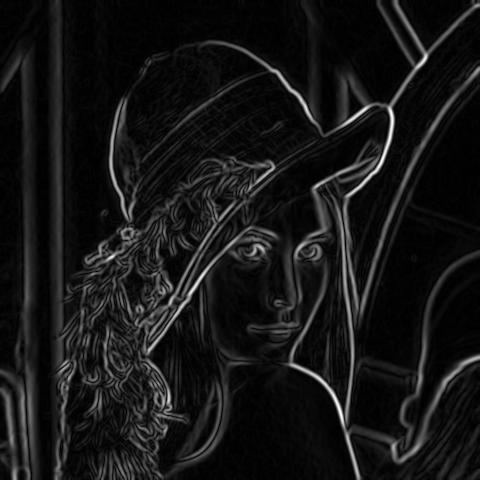
\includegraphics[width=0.5\textwidth]{images/gmag.jpg}
            \caption{Εφαρμογή τελεστή Sobel για εύρεση κατευθυντικών παραγώγων}
            \label{fig:gmag}
        \end{figure}
        \item Βήμα 3: Non Maximum Suppresion (απαλοιφή των μη-µεγίστων) για την διατήρηση μόνο των έντονων ακμών.
        \begin{figure}[H]
            \centering
            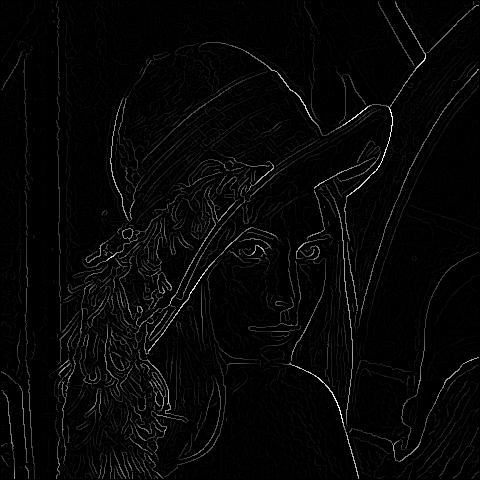
\includegraphics[width=0.5\textwidth]{images/non_maximum_suppression.jpg}
            \caption{Εφαρμογή Non Maximum Suppresion}
            \label{fig:non-maxima}
        \end{figure}
        \item Βήμα 4: Εφαρμογή κατωφλίωσης (double thresholding) για τον περαιτέρω διαχωρισμό των αχνών ακμών.
        \begin{figure}[H]
            \centering
            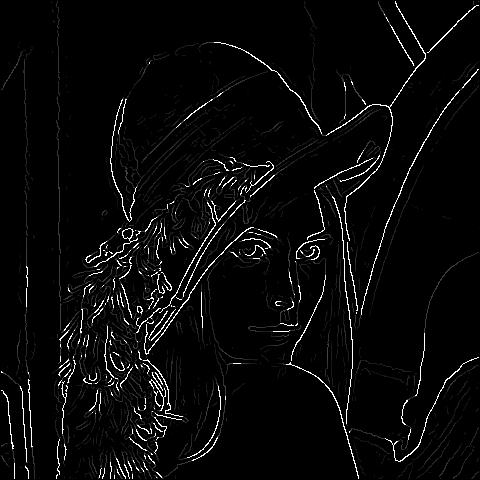
\includegraphics[width=0.5\textwidth]{images/double_threshold.jpg}
            \caption{Εφαρμογή Double Thresholding}
            \label{fig:double-thresholding}
        \end{figure}
        \item Βήμα 5: Αφού έχουμε διαχωρίσει τις έντονες από τις αχνές ακμές, εφαρμόζουμε κατωφλίωση των ακμών με υστέρηση, δηλαδή διατήρηση μόνο των έντονων ακμών και των αχνών ακμών που συνδέονται με έντονες. Αυτό παράγει μια εικόνα στην οποία φαίνονται μόνο οι ακμές που αντιστοιχούν σε πραγματικές γραμμές.
        \begin{figure}[H]
            \centering
            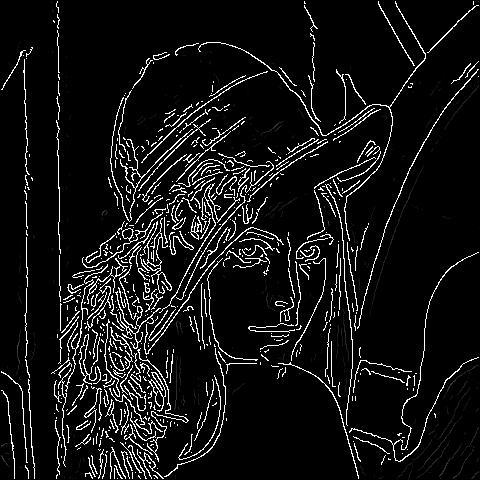
\includegraphics[width=0.5\textwidth]{images/edge_tracking.jpg}
            \caption{Εφαρμογή κατωφλίωσης με υστέρηση}
            \label{fig:thresholding-hysterisis}
        \end{figure}
    \end{itemize}
    \item \emph{Hough Transform}: Ο μετασχηματισμός Hough είναι μια ευρύτερη μέθοδος εντοπισμού χαρακτηριστικών συγκεκριμένου σχήματος μέσα σε μια εικόνα \cite{wiki:hough}. Επειδή τα επιθυμητά χαρακτηριστικά πρέπει να βρίσκονται σε κάποια παραμετρική μορφή, ο κλασσικός μετασχηματισμός Hough χρησιμοποιείται συχνά για τον εντοπισμό καμπύλων, όπως ευθείες γραμμές, κύκλοι, ελλείψεις κλπ. Τα βασικότερα πλεονεκτήματα του μετασχηματισμού αυτού είναι ότι είναι αρκετά αποτελεσματικός ακόμα και σε επικαλυπτόμενα αντικείμενα (δηλαδή είναι ανεκτικός στην έλλειψη κομματιών από μια ευθεία) και παράλληλα δεν επηρεάζεται πολύ από τον θόρυβο που υπεισέρχεται στην εικόνα. Στα πλαίσια της παρούσας διπλωματικής επιλέχθηκε η χρήση του μετασχηματισμού Hough για εντοπισμό παράλληλων γραμμών. Η βασική ιδέα της μεθόδου είναι ότι μετατρέπει τα σημεία από καρτεσιανές συντεταγμένες $(x,y)$ σε πολικές $(\rho,\theta)$ και έπειτα χρησιμοποιεί μια διαδικασία ψηφοφορίας για την ανάδειξη των υποψήφιων σχημάτων στην εικόνα.
    \begin{figure}[H]
        \centering
        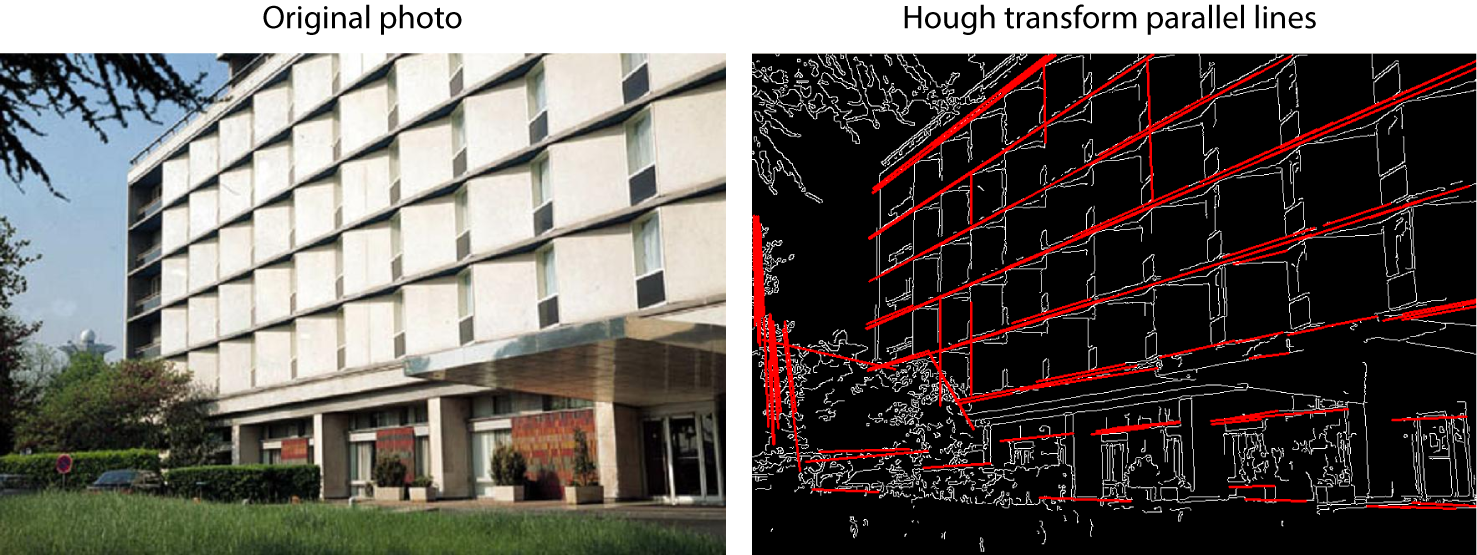
\includegraphics[width=\textwidth]{images/Hough_transform_example.png}
        \caption{Εφαρμογή Hough Transform}
        \label{fig:hough-transform-example}
    \end{figure}
\end{itemize}

\paragraph{Block-Based Recognition}\label{block-based}
Το κομμάτι του Block-Based Recognition περιλαμβάνει την προ-επεξεργασία και τον εντοπισμό παράλληλων γραμμών. Χρησιμοποιείται για να υπολογιστούν οι γωνίες των παράλληλων γραμμών και για να καταγραφούν τα σκορ κάθε pixel στα blocks.
\begin{enumerate}[1)]
    \item \emph{Προ-επεξεργασία}: Η φάση αυτή περιλαμβάνει τα εξής 4 βήματα:
    \begin{itemize}
        \item Βήμα 1: Μετατροπή του block από έγχρωμο σε κλίμακα του γκρι (grayscale), επειδή οι γραμμές της διάβασης σε μια εικόνα κλίμακας του γκρι φαίνονται ως σκούρες και φωτεινές λωρίδες.
        \item Βήμα 2: Εφαρμόζεται η μέθοδος προσαρμοστικού κατωφλίου (adaptive thresholding), η οποία αποδίδει σε ένα pixel μια δυαδική τιμή (0 ή 1) ανάλογα με το αν η τιμή του pixel είναι μεγαλύτερη από ένα μεταβλητό κατώφλι. Η διαδικασία αυτή βοηθάει να περιοριστεί το φαινόμενο της σκίασης στις εικόνες.
        \item Βήμα 3: Εφαρμογή των μορφολογικών μετασχηματισμών Διαστολής (Dilation) και Διάβρωσης (Erosion) για εξομάλυνση των ορίων.
        \item Βήμα 4: Εφαρμογή του φίλτρου Canny Edge Detector για να ανιχνευθούν οι ακμές που υπάρχουν στο block.
    \end{itemize}
    
    \item \emph{Εντοπισμός παράλληλων γραμμών}: Εφαρμόζεται ο Μετασχηματισμός Hough για να εντοπιστούν οι παράλληλες γραμμές στο block. Ορίζεται τοπικά ως αρχή των αξόνων η πάνω αριστερή γωνία του block και κάθε μη-μηδενικό pixel που ανήκει σε ακμή μετασχηματίζεται από το καρτεσιανό στο πολικό σύστημα συντεταγμένων με την παρακάτω εξίσωση:$$\rho = x\cos{\theta}+y\sin{\theta},$$ όπου η συντεταγμένη $\rho$ αναπαριστά την απόσταση της αρχής των αξόνων από την ευθεία γραμμή που διέρχεται από το $(x,y)$, και το η συντεταγμένη $\theta$ αναπαριστά την γωνία μεταξύ του κάθετου στη γραμμή διανύσματος (normal) και του άξονα x. Η αναζήτηση περιορίζεται σε παράλληλες γραμμές που βρίσκονται στο εύρος [-30\degree, +30\degree], δηλαδή ψάχνουμε μόνο για $\theta \in [60\degree,120\degree]$, επιλέγοντας διακριτές τιμές του $\theta$. Ανάλογα με τις πολικές συντεταγμένες $(\rho,\theta)$ που ικανοποιούν κάθε pixel ακμής, δημιουργείται ένας πίνακας συσσώρευσης (Σχήμα \ref{fig:voting-hough}). Το πλεονέκτημα του Block-Based Μετασχηματισμού Hough είναι ότι φιλτράρει τυχόν σημεία που έχουν υπεισέλθει στις ακμές λόγω θορύβου. Περιληπτικά, τα βήματα που ακολουθούνται για την εξαγωγή των παράλληλων γραμμών είναι τα παρακάτω:
    \begin{itemize}
        \item Βήμα 1: Σε κάθε block, ακολουθείτε μια διαδικασία ψηφοφορίας κατά την οποία κάθε ζεύγος $(\rho,\theta)$, που αντιστοιχεί σε ένα pixel ακμής, αντιστοιχίζεται σε μια θέση στον πίνακα συσσώρευσης (Σχήμα \ref{fig:voting-hough}). Κάθε φορά που ένα τέτοιο ζεύγος εντοπίζεται, η τιμή της αντίστοιχης θέσης στον πίνακα συσσώρευσης αυξάνεται κατά 1. Με άλλα λόγια κάθε pixel ακμής "ψηφίζει" για τις αντίστοιχες θέσεις (ζεύγος $(\rho,\theta)$) που ικανοποιούν την εξίσωση του. Κάθε θέση με παραπάνω από 1 ψήφους θεωρείται μια ευθεία γραμμή στις καρτεσιανές συντεταγμένες.
        \item Βήμα 2: Επιλέγονται οι 10 θέσεις με τις περισσότερες ψήφους. Η γωνία $\theta$ με τις περισσότερες ψήφους επιλέγεται ως η γωνία ανάμεσα στο κάθετο διάνυσμα της υποψήφιας παράλληλης γραμμής και του άξονα x.
        \item Βήμα 3: Εξάγονται όλες οι γραμμές των οποίων η γωνία είναι ίση με την γωνία που επιλέχθηκε στο προηγούμενο βήμα και η παραλληλία επιβεβαιώνεται εάν υπάρχουν τουλάχιστον 3 ευθείες γραμμές, των οποίων το πλήθος των ψήφων είναι μεγαλύτερο από 60.
    \end{itemize}
\end{enumerate}
\begin{figure}[H]
    \centering
    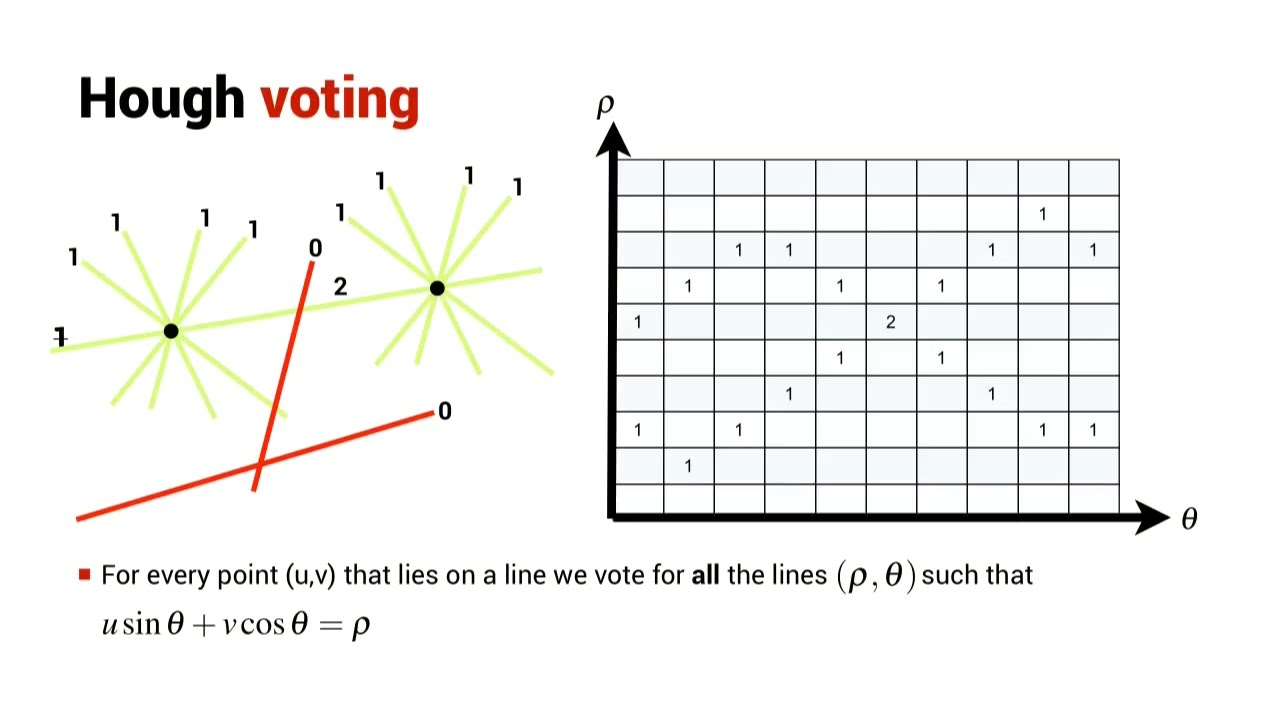
\includegraphics[width=\textwidth]{images/hough_transform.jpg}
    \caption{Παράδειγμα δημιουργίας πίνακα συσσώρευσης κατά τον μετασχηματισμό Hough \cite{FindingL66:online}. Κάθε θέση στον πίνακα εκφράζει μια ευθεία και κάθε ψήφος σε μια θέση εκφράζει τον αριθμό των σημείων από τα οποία διέρχεται αυτή η ευθεία.}
    \label{fig:voting-hough}
\end{figure}

\paragraph{Synthesize}\label{synthesize}
Αφού έχουν αναλυθεί όλα τα blocks, η τελική γωνία $\theta$ μεταξύ των παράλληλων γραμμών και του άξονα x υπολογίζεται ως αυτή με τους περισσότερους ψήφους ανά block. Τα σκορ των pixels αξιολογούνται για να εξαχθεί ένα ασφαλές μονοπάτι που να αντιστοιχεί στη διάβαση. Τα pixels με μεγαλύτερο σκορ αντιπροσωπεύουν μονοπάτι με μεγαλύτερη ασφάλεια.

\begin{figure}[H]
    \centering
    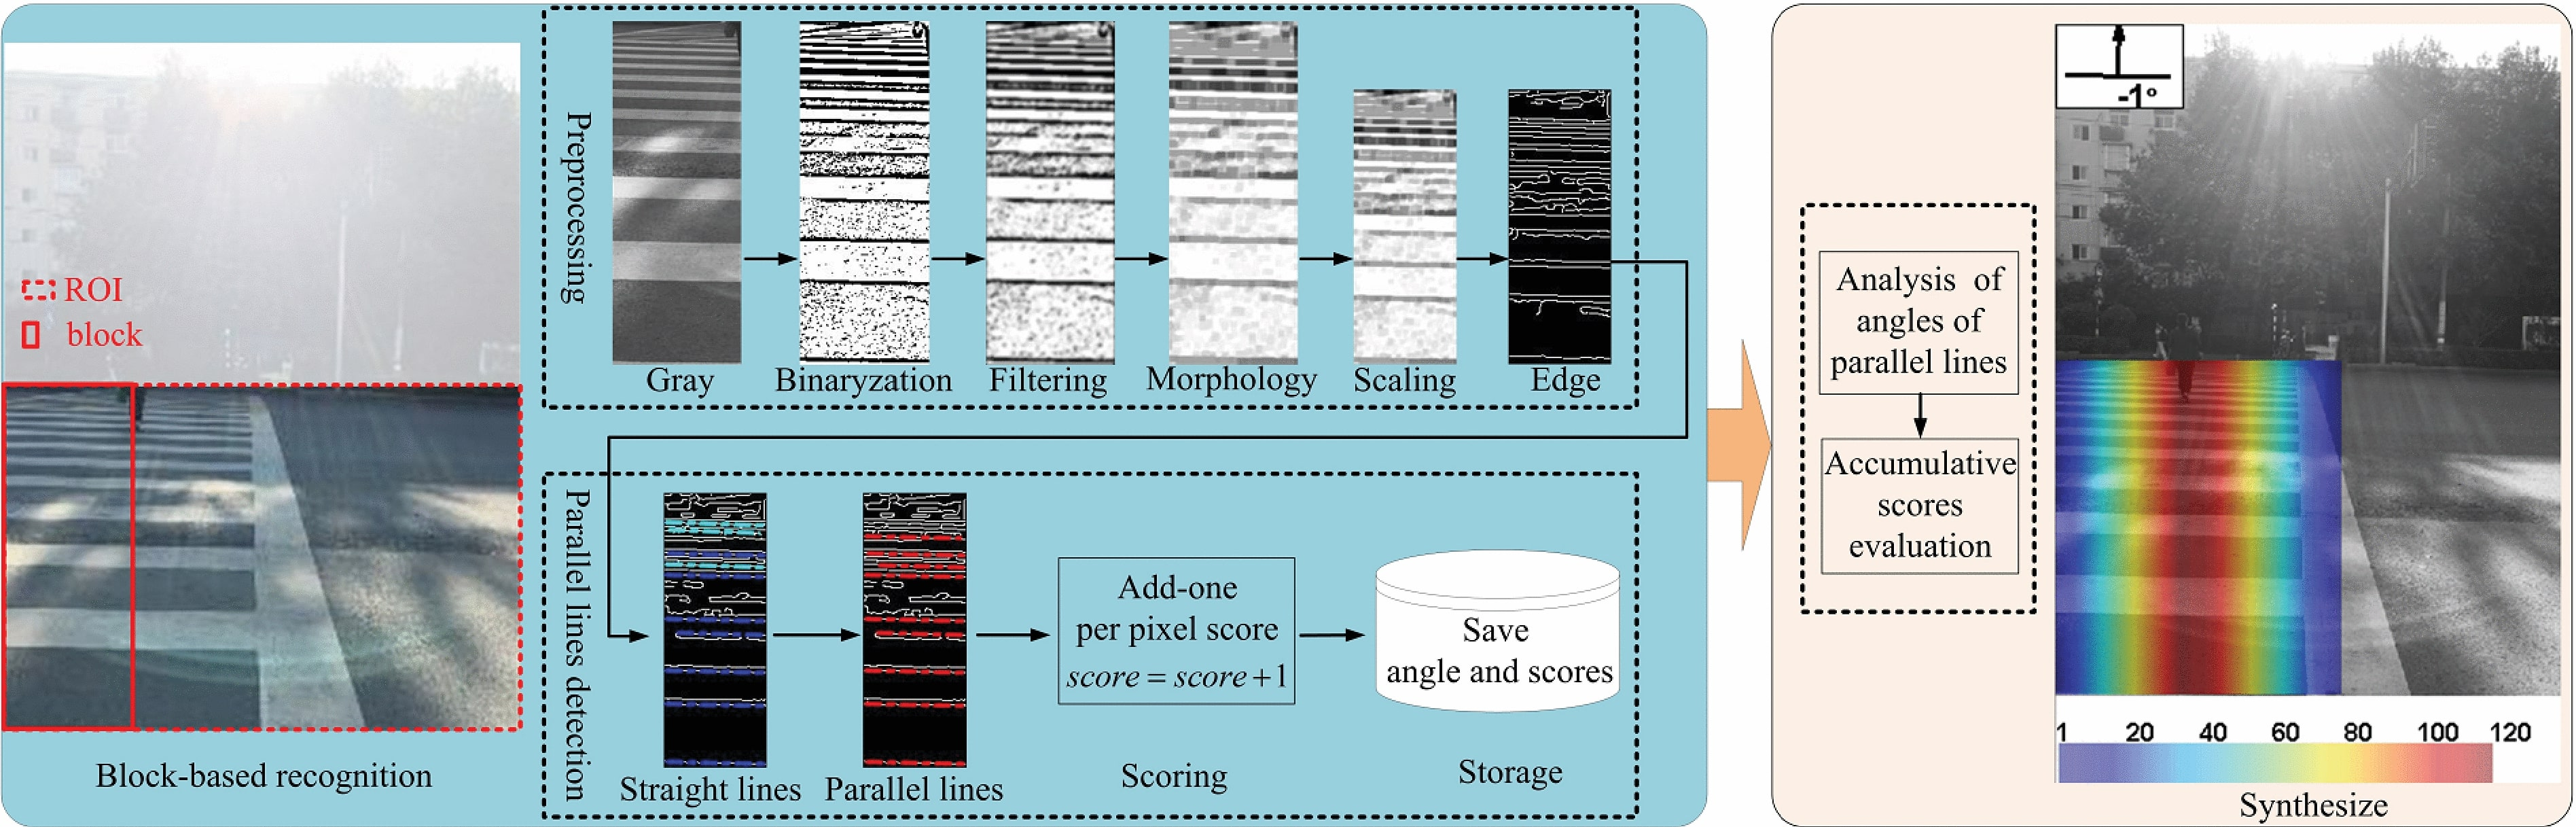
\includegraphics[width=\textwidth]{images/flow_hough_paper.jpg}
    \caption{Overview του αλγόριθμου εντοπισμού διάβασης πεζών που παρουσιάζεται στην ερευνητική εργασία \cite{wu_block-based_2019}}
    \label{fig:flow-hough-paper}
\end{figure}

\subsubsection{Αναγνώριση φωτεινού σηματοδότη}
Αν το σύστημα ανιχνεύσει διάβαση πεζών τότε καλείται ο αλγόριθμος αναγνώρισης φωτεινού σηματοδότη. Ο αλγόριθμος αυτός είναι υπεύθυνος για τον εντοπισμό του φαναριού στην εικόνα και την αναγνώριση του χρώματος (πράσινο ή κόκκινο). Η βασική ιδέα του αλγορίθμου βασίζεται στην μέθοδο του \emph{Spot Light Detection} (ανίχνευση σημειακών πηγών φωτός), η οποία εκμεταλλεύεται το γεγονός ότι οι τα φανάρια είναι αυτόφωτα, δηλαδή είναι πηγές φωτός, για να μπορέσει να εντοπίσει τη θέση τους μέσα σε μια εικόνα. Στη συνέχεια, αφού εντοπιστούν οι θέσεις της εικόνας με τους υποψήφιους φωτεινούς σηματοδότες, ορίζεται ένα bounding box (περίγραμμα) γύρω από αυτά και κάθε τέτοιο bounding box συγκρίνεται με ένα προκαθορισμένο template φωτεινού σηματοδότη. Αν το αποτέλεσμα τη σύγκρισης είναι μεγαλύτερο από ένα κατώφλι (\emph{φάση επαλήθευσης}), που ορίζεται από τον χρήστη, τότε το συγκεκριμένο bounding box, και συνεπώς η συγκεκριμένη θέση στην εικόνα, αναπαριστά έναν φωτεινό σηματοδότη. Για να γίνει αναγνώριση του κόκκινου και του πράσινου χρώματος, έχουν οριστεί δύο διαφορετικά templates που αντιπροσωπεύουν το κόκκινο και το πράσινο φανάρι.

\begin{figure}[H]
    \centering
    
\includegraphics[width=\textwidth]{images/tl_system_overview.png}
    \caption{Overview του αλγόριθμου αναγνώρισης φωτεινών σηματοδοτών}
    \label{fig:tl-overview}
\end{figure}

\paragraph{Spot Light Detection}
Σκοπός του συγκεκριμένου βήματος είναι η εξαγωγή των περιοχών της αρχικής εικόνας, που είναι υποψήφιες να περιέχουν φωτεινό σηματοδότη. Η υλοποίηση του αλγορίθμου βασίστηκε σε ορισμένες ερευνητικές δημοσιεύσεις σχετικά με τον εντοπισμό φωτεινών σηματοδοτών σε εφαρμογές αυτόνομης οδήγησης \cite{de2009real, tae2006detection} και έχει την ακόλουθη δομή:
\begin{itemize}
    \item Βήμα 1: Αρχικά, όπως και στον αλγόριθμο εντοπισμού διάβασης πεζών, έτσι κι εδώ διαιρούμε την αρχική εικόνα ορίζοντας μια περιοχή ενδιαφέροντος που αντιστοιχεί στο πάνω 40\% τμήμα της αρχικής εικόνας και στο 80\% πλάτος. Αυτό συμβαίνει για να επιταχύνουμε τον αλγόριθμο, γνωρίζοντας ότι οι φωτεινοί σηματοδότες βρίσκονται σχεδόν πάντα στο πάνω κεντρικό τμήμα μιας εικόνας.
    \begin{figure}[H]
        \centering
        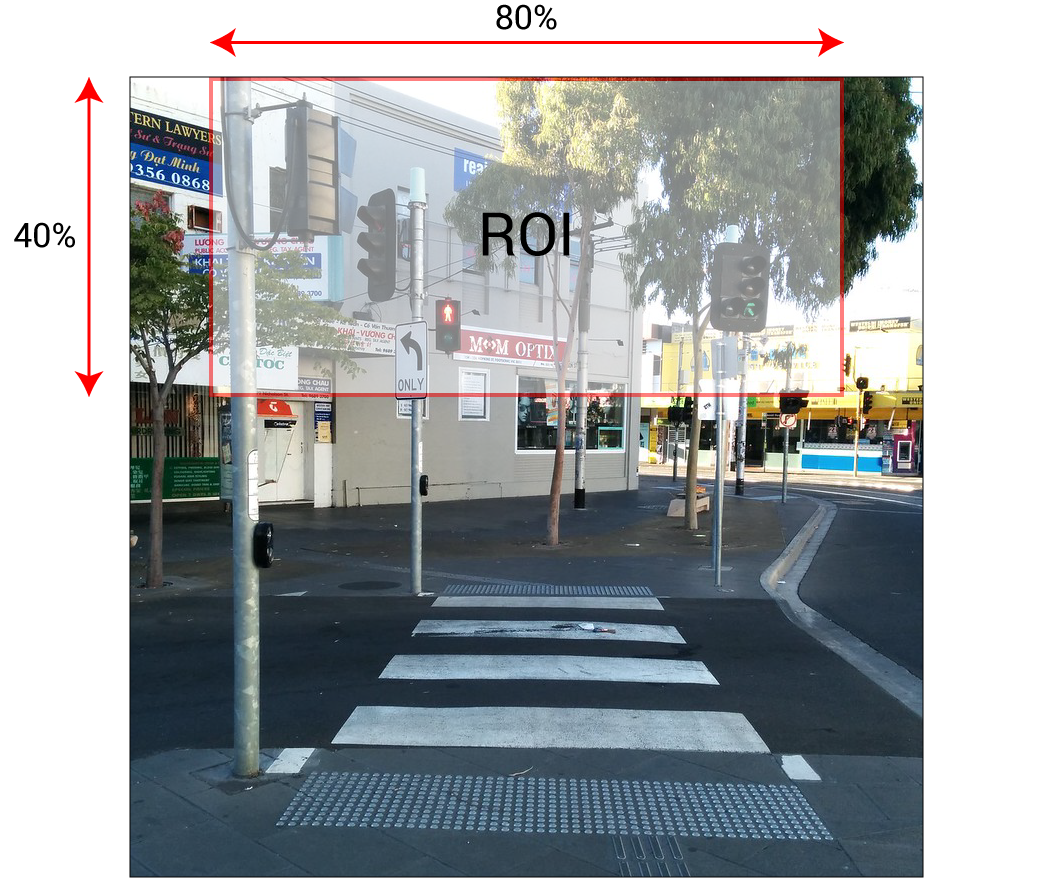
\includegraphics[width=0.6\textwidth]{images/upper_roi.png}
        \caption{Επιλογή περιοχής ενδιαφέροντος (ROI) για αναγνώριση φωτεινού σηματοδότη}
        \label{fig:upper-roi}
    \end{figure}
    \item Βήμα 2: Στη συνέχεια μετατρέπουμε την εικόνα από έγχρωμη σε κλίμακα του γκρι.
    \item Βήμα 3: Αφαίρεση θορύβου με εφαρμογή του \emph{μορφολογικού μετασχηματισμού Top-hat} \cite{wiki:top_hat}. Γενικά, η αρχική εικόνα μπορεί να περιέχει αρκετό θόρυβο που προέρχεται από παραμόρφωση του φακού, αντανάκλαση του ηλιακού φωτός, δόνηση της κάμερας και αντικείμενα φόντου με παρόμοιο χρώμα. Αυτός ο θόρυβος μπορεί να περιοριστεί με την εφαρμογή μορφολογικών μετασχηματισμών. Πιο συγκεκριμένα, μετασχηματισμός Top-hat ανήκει σε μια ευρύτερη οικογένεια μορφολογικών μετασχηματισμών που χρησιμοποιούν ένα δομικό στοιχείο (structuring element) το οποίο εφαρμόζεται στην αρχική εικόνα και βάσει αυτού οι τιμές των pixels αλλάζουν ανάλογα με τις τιμές των γειτονικών pixels. Γενικά το δομικό στοιχείο είναι απλού γεωμετρικού σχήματος και μεγέθους μικρότερου από το σχήμα το οποίο θα επεξεργαστεί. Υπάρχουν διάφορα σχήματα δομικών στοιχείων που μπορούν να εφαρμοστούν, τα πιο γνωστά είναι το τετράγωνο,ο σταυρός, ο δίσκος και η γραμμή. Οι μορφολογικοί τελεστές έχουν διάφορες εφαρμογές. Απλές εφαρμογές τους είναι το φιλτράρισμα, η ανίχνευση χαρακτηριστικών, η λέπτυνση, η ενίσχυση της αντίθεσης κ.α. Στην προκειμένη περίπτωση χρησιμοποιείται ένα δομικό στοιχείο σε σχήμα τετραγώνου και επιλέχθηκε ο μετασχηματισμός White Top-hat, ο οποίος επιστρέφει μια εικόνα που περιέχει τα "αντικείμενα" που είναι "μικρότερα" από το δομικό στοιχείο και πιο φωτεινά από το περιβάλλον τους. Με αυτόν τον τρόπο δίνεται έμφαση στις φωτεινές πηγές της εικόνας, όπως οι φωτεινοί σηματοδότες.
    \item Βήμα 4: Τέλος, γίνεται εξαγωγή των υποψήφιων περιοχών με χρήστη της μεθόδου Blob Detection. Ως blob ορίζεται ένα γκρουπ από συνδεδεμένα pixels που μοιράζονται κάποια κοινά χαρακτηριστικά, π.χ. έχουν την ίδια χρωματική τιμή, και στόχος της μεθόδου blob detection είναι να αναγνωρίσει και να προσδιορίσει αυτές τις περιοχές. Η OpenCV περιέχει μια κλάση, την \emph{SimpleBlobDetector}, η οποία υλοποιεί την μέθοδο Blob Detection. Ο αλγόριθμος που χρησιμοποιείται από την OpenCV, προσδιορίζει τα blobs με βάση τις παρακάτω παραμέτρους:
    \begin{itemize}
        \item Μέγεθος: φιλτράρισμα των περιοχών με βάση το εμβαδόν τους σε pixels.
        \item Circularity: παράμετρος που καθορίζει την ομοιότητα του αντικειμένου με κύκλο.
        \item Convexity: με τον όρο αυτόν εννοούμε την κυρτότητα του αντικειμένου και το φίλτρο αυτό καθορίζει τον ελάχιστο και μέγιστο βαθμό κυρτότητας.
        \begin{figure}[H]
            \centering
            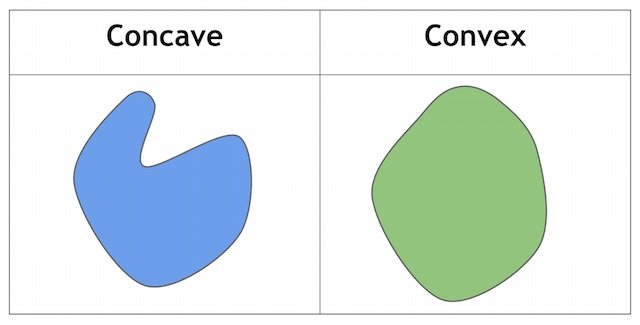
\includegraphics[width=0.6\textwidth]{images/concave-convex.jpg}
            \caption{Παράδειγμα ιδιότητας convexity}
            \label{fig:convex}
        \end{figure}
        \item Inertia Ratio: αυτή η παράμετρος μετράει το πόσο επίμηκες είναι ένα αντικείμενο.
        \begin{figure}[H]
            \centering
            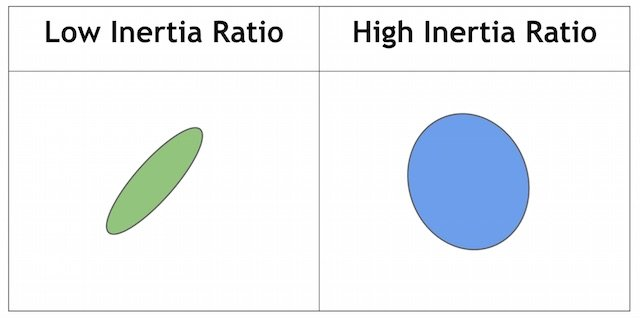
\includegraphics[width=0.6\textwidth]{images/inertia.jpg}
            \caption{Παράδειγμα ιδιότητας inertia ratio}
            \label{fig:inertia}
        \end{figure}
    \end{itemize}
\end{itemize}

\paragraph{Template Matching}
Template matching ονομάζεται η τεχνική εύρεσης περιοχών μιας εικόνας, που ταιριάζουν, ή είναι παρόμοιες, με μια δοθείσα εικόνα-πρότυπο. Αφού έχουν εντοπιστεί οι περιοχές που είναι υποψήφιες να περιέχουν κάποιον φωτεινό σηματοδότη, λαμβάνει χώρα το επόμενο στάδιο το οποίο περιλαμβάνει σύγκριση των περιοχών αυτών με κάποια προεπιλεγμένα templates φωτεινών σηματοδοτών. Σε αυτό το σημείο πρέπει να γίνει ξεκάθαρο ότι η σύγκριση γίνεται ανάμεσα στα πρότυπα και στην έγχρωμη αρχική εικόνα. Οι υποψήφιες περιοχές που βρέθηκαν προηγουμένως αντιστοιχούνται στην αρχική έγχρωμη εικόνα. Μετά από πειραματικές προσπάθειες βρέθηκε ότι τα templates που παρουσιάζουν μεγαλύτερη αποτελεσματικότητα είναι αυτά που φαίνονται στο σχήμα \ref{fig:templates}. Προϋπόθεση για να γίνει το template matching είναι το δοθέν πρότυπο να είναι μικρότερο σε διαστάσεις από την εικόνα προς σύγκριση. Πριν πραγματοποιηθεί η σύγκριση, εφαρμόζεται γκαουσιανό φίλτρο για την εξομάλυνση του προτύπου και το φιλτράρισμα τυχόν θορύβου. Στα πλαίσια της παρούσας διπλωματικής, στόχος ήταν να βρούμε την ομοιότητα του κόκκινου και πράσινου προτύπου με μια περιοχή της εικόνας. Αν μια υποψήφια περιοχή είχε βαθμό ομοιότητας με οποιοδήποτε πρότυπο πάνω από ένα συγκεκριμένο κατώφλι, τότε λέμε ότι αναπαριστά έναν φωτεινό σηματοδότη. Επιπλέον, συγκρίνεται η ομοιότητα με το πράσινο και το κόκκινο πρότυπο ξεχωριστά για να γίνει η αναγνώριση του χρώματος του φαναριού. Η διαδικασία ελέγχου του αποτελέσματος των συγκρίσεων με τα προκαθορισμένα κατώφλια καλείται \textbf{φάση \emph{επαλήθευσης (validation)}}.

Η σύγκριση γίνεται \emph{ολισθαίνοντας} την εικόνα-πρότυπο πάνω από την αρχική εικόνα. Με τον όρο ολίσθηση υποδηλώνεται η μετακίνηση της εικόνας-προτύπου κατά ένα pixel τη φορά (από τα αριστερά στα δεξιά, από πάνω προς τα κάτω). Σε κάθε θέση υπολογίζεται ένα μέτρο ομοιότητας που αντιπροσωπεύει το ποσοστό της ομοιότητας του προτύπου $T$ με την συγκεκριμένη περιοχή της αρχικής εικόνας $I$. Η τιμή αυτή του μέτρου για κάθε pixel αποθηκεύεται σε μια νέα εικόνα $R$, η οποία αποτελεί την εικόνα μετρήσεων (σχήμα \ref{fig:template-result}). Υπάρχουν διάφορες διαθέσιμες μέθοδοι μέτρησης της ομοιότητας \cite{Template98:online}. Στην προκειμένη περίπτωση χρησιμοποιήθηκε η μέθοδος \emph{Sum of Square Differences (SSD) Normed} η οποία υπολογίζει την ομοιότητα βάσει της παρακάτω εξίσωσης:\[R(x,y)=\frac{\sum_{x',y'}(T(x',y')-I(x+x',y+y'))^2}{\sqrt{\sum_{x',y'}T(x',y')^2\cdot \sum_{x',y'}I(x+x',y+y')^2}}\]
\begin{figure}[H]
    \centering
    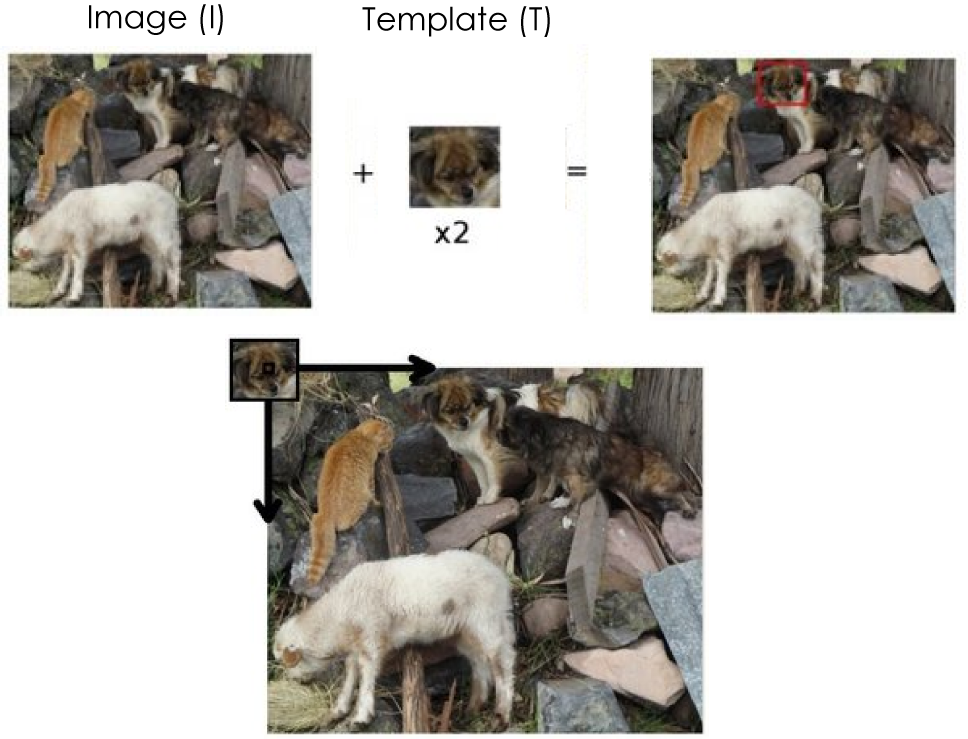
\includegraphics[width=0.6\textwidth]{images/template_matching.png}
    \caption{Overview της διαδικασίας template matching}
    \label{fig:template-matching}
\end{figure}

\begin{figure}[H]
    \centering
    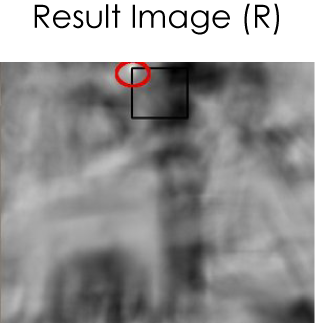
\includegraphics[width=0.4\textwidth]{images/template_result.png}
    \caption{Το αποτέλεσμα της διαδικασίας ολίσθησης βάσει της μετρικής Cross Correlation Normed (TM\textunderscore CCORR\textunderscore NORMED). Οι φωτεινές περιοχές υποδεικνύουν μεγαλύτερη ομοιότητα. Η θέση με τον κόκκινο κύκλο είναι αυτή με την υψηλότερη τιμή, γιαυτό η περιοχή με το περίγραμμα θεωρείται ως αυτή με το καλύτερο ταίριασμα.}
    \label{fig:template-result}
\end{figure}

\begin{figure}[H]
    \centering
    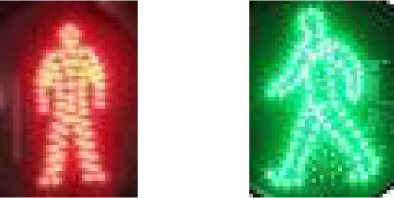
\includegraphics[width=0.5\textwidth]{images/templates.png}
    \caption{Τα templates που χρησιμοποιήθηκαν στην παρούσα εργασία}
    \label{fig:templates}
\end{figure}

\paragraph{Περισσότερα σχετικά με τους μορφολογικούς μετασχηματισμούς}
Οι μορφολογικοί μετασχηματισμοί είναι κάποιες διεργασίες που αποσκοπούν στην εξαγωγή ορισμένων χαρακτηριστικών από τις εικόνες στις οποίες εφαρμόζονται \cite{zacharia2013}. Όπως προαναφέρθηκε, σε αυτές τις διεργασίες υπάρχει ένα δομικό στοιχείο (structuring element) το οποίο είναι ουσιαστικά ένας πίνακας οποιασδήποτε διάστασης που περιέχει 0 και 1. Γενικά, το δομικό στοιχείο είναι απλού γεωμετρικού σχήματος (τετράγωνο, σταυρός, δίσκος, γραμμή) και μεγέθους μικρότερου από το σχήμα το οποίο θα επεξεργαστεί. Κάποιες από τις βασικές διεργασίες μορφολογικών μετασχηματισμών είναι οι παρακάτω \cite{OpenCVMo48:online}:
\begin{itemize}
    \item \textbf{Διαστολή (Dilation)}: Η διαστολή επεκτείνει τα αντικείμενα της εικόνας και παράλληλα κλείνει τις τρύπες που υπάρχουν. Γι' αυτό το λόγο είναι επεκτατικό φίλτρο. Αυτό που συμβαίνει είναι ότι η διαστολή τοποθετεί το δομικό στοιχείο στην εικόνα και το μετακινεί μέσα σε αυτή με τρόπο παρόμοιο με αυτόν της συνέλιξης.
    \item \textbf{Συστολή (Erosion)}: H συστολή είναι το δυαδικό συμπλήρωμα η διαστολή. Η διαδικασία που εκτελεί είναι παρόμοια με τη διαστολή, μόνο που αυτό αντί να επεκτείνει τα αντικείμενα της εικόνας, τα μικρύνει, κόβοντας παράλληλα της κορυφές των περιγραμμάτων των σχημάτων και γι' αυτό το λόγο είναι μη επεκτατικό φίλτρο.
    \item \textbf{Άνοιγμα (Opening)}: Το φίλτρο ανοίγματος αποτελεί συνδυασμό της διαστολής και της συστολής. Πιο συγκεκριμένα, υποδηλώνει μια διεργασία στην οποία ένα αντικείμενο υπόκειται πρώτα σε συστολή και αμέσως μετά σε διαστολή. Ανήκει στα μη επεκτατικά φίλτρα και χρησιμοποιείται για την αφαίρεση των μικρών αντικειμένων (που συνήθως είναι τα πιο φωτεινά) από το προσκήνιο.
    \item \textbf{Κλείσιμο (Closing)}: Αντίστοιχα, το φίλτρο κλεισίματος αποτελεί τον ανάποδο συνδυασμό από το άνοιγμα, δηλαδή πρώτα διαστολή και αμέσως μετά συστολή. Ανήκει στα επεκτατικά φίλτρα και χρησιμοποιείται για την αφαίρεση των μικρών οπών (συνήθως μαύρου χρώματος) από το προσκήνιο.
    \item \textbf{Top-Hat}: Όπως εξηγήθηκε και πιο πάνω, ο μετασχηματισμός Top-Hat χρησιμοποιείται στην επεξεργασία εικόνας για την εξαγωγή χαρακτηριστικών, την εξίσωση του φόντο, την ενίσχυση της αντίθεσης της εικόνας, την απομάκρυνση αντικειμένων από μια εικόνα κ.α. Στον Top-Hat μετασχηματισμό γίνεται είτε η αφαίρεση του αρχικού σήματος με το άνοιγμα του εαυτού του ($ I - Opening(I)$), το οποίο ονομάζεται και white Top-Hat transform, ή η αφαίρεση του κλεισίματος του σήματος με το αρχικό σήμα ($Closing(I)-I$), το οποίο ονομάζεται και ως black Top-Hat transform.
\end{itemize}
\begin{figure}[H]
    \centering
    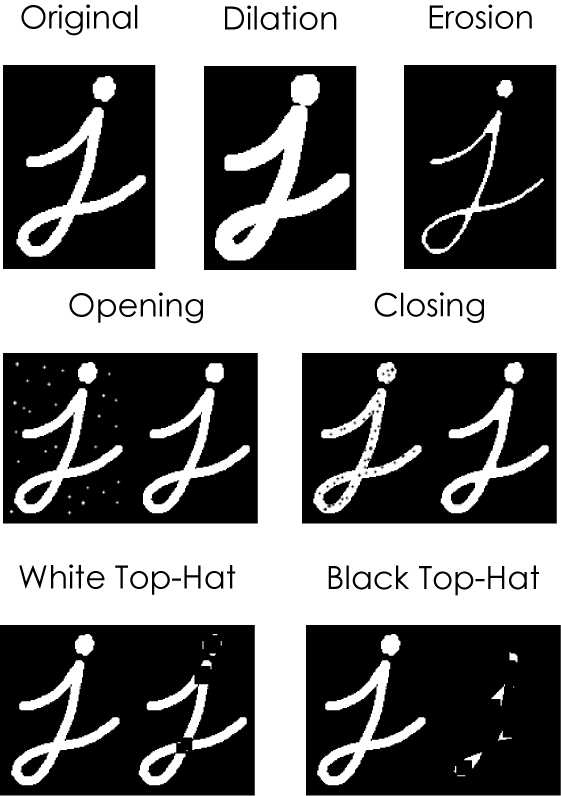
\includegraphics[width=0.5\textwidth]{images/morph_operations.png}
    \caption{Παράδειγμα μορφολογικών διεργασιών}
    \label{fig:morph-operations}
\end{figure}

\subsubsection{Αλγόριθμος εντοπισμού εμποδίων}
Το τρίτο και τελευταίο μέρος του προτεινόμενου συστήματος πλοήγησης για άτομα με προβλήματα όρασης είναι ο αλγόριθμος εντοπισμού φυσικών εμποδίων. Ο αλγόριθμος αυτός τρέχει καθ' όλη την διάρκεια της πλοήγησης του χρήστη και χρησιμοποιεί τον ενσωματωμένο αισθητήρα βάθους της κάμερας για να αποφασίσει σχετικά με την ύπαρξη ή όχι εμποδίων μπροστά από τον χρήστη.

Η βασική ιδέα πίσω από την υλοποίηση τους συγκεκριμένου αλγόριθμου είναι αρκετά απλή. Αρχικά, λαμβάνεται η εικόνα βάθους από την κάμερα και αφού περάσει τη φάση της προ-επεξεργασίας, που αναφέραμε στην αρχή της ενότητας, εφαρμόζεται ακόμα ένα στάδιο υπο-δειγματοληψίας, με σκοπό να μειώσουμε κι άλλο το υπολογιστικό κόστος. Πιο συγκεκριμένα, οι διαστάσεις τις εικόνας μειώνονται στο μισό. Ο λόγος που εφαρμόζουμε υπο-δειγματοληψία είναι ότι στον συγκεκριμένο αλγόριθμο δεν παίζει σημαντικό ρόλο η λεπτομέρεια στην εικόνα βάθους. Το ζητούμενο είναι να εντοπιστούν μεγάλοι, ή σχεδόν μεγάλοι, όγκοι αντικειμένων μπροστά από τον χρήστη, που εμποδίζουν την διέλευσή του από το συγκεκριμένο μονοπάτι. Έτσι, η ελάττωση της λεπτομέρειας της εικόνας βάθους που επάγεται από την υπο-δειγματοληψία δεν επηρεάζει την αποτελεσματικότητα του αλγορίθμου. Τα εμπόδια που εντοπίζονται έχουν μέγιστη απόσταση από την κάμερα 1 μέτρο. Αυτό υλοποιείται εφαρμόζοντας ένα φίλτρο αποκοπής, όπου μηδενίζει όλα τα pixels που έχουν τιμή κάτω από ένα όριο, το οποίο αντιστοιχεί σε απόσταση 1μ.

Στη συνέχεια, η εικόνα διαιρείτε σε 3 υπο-περιοχές: την αριστερή, την κεντρική και την δεξιά περιοχή. Ο αλγόριθμος ελέγχει συνεχώς την κεντρική περιοχή για τυχόν εμπόδια. Αν βρεθεί εμπόδιο στην κεντρική περιοχή τότε εξετάζει την αριστερή περιοχή και αν είναι ελεύθερη από εμπόδια, ειδοποιεί τον χρήστη να μετακινηθεί προς τα αριστερά. Σε περίπτωση που υπάρχει εμπόδιο και στην αριστερή περιοχή, τότε ελέγχεται η δεξιά πλευρά και ακολούθως ο χρήστης ειδοποιείται κατάλληλα. Εάν όλες οι υπο-περιοχές είναι κατειλημμένες από εμπόδια, τότε ο αλγόριθμος φτάνει σε αδιέξοδο και περιμένει την ελευθέρωση κάποιας περιοχής. Συνήθως τέτοια εμπόδια είναι δυναμικής φύσεως, δηλαδή πρόκειται για κάποιον περαστικό, ο οποίος μετά από μερικά δευτερόλεπτα θα έχει φύγει από το οπτικό πεδίο της κάμερας κι έτσι ο αλγόριθμος θα ανακαλύψει το ελεύθερο μονοπάτι που υπάρχει. Η προτεραιότητα που δίνεται στην αριστερή περιοχή είναι καθαρά αυθαίρετη επιλογή και μπορεί κάλλιστα να τροποποιηθεί.

Η ανίχνευση των εμποδίων σε κάποια υπο-περιοχή γίνεται χρησιμοποιώντας την μέθοδο blob detection, που περιγράφηκε στην προηγούμενη ενότητα. Πιο συγκεκριμένα, η μοναδική παράμετρος που χρησιμοποιείται για την ανίχνευση εμποδίου είναι το μέγεθός του. Δεδομένου ότι η εικόνα βάθους που λαμβάνεται από την κάμερα είναι σε κλίμακα του γκρι και οι κοντινότερες περιοχές αναπαριστώνται με φωτεινότερες αποχρώσεις, η μέθοδος blob detection απομονώνει τα pixels που έχουν τιμή μεγαλύτερη από ένα συγκεκριμένο κατώφλι (π.χ. μεγαλύτερη από 100) και στη συνέχεια αναζητά ομάδες από pixels που σχηματίζουν ένα ενιαίο αντικείμενο με εμβαδόν ανάμεσα στα όρια που έχουν θεσπιστεί στον αλγόριθμο. Αν εντοπιστεί κάποιο αντικείμενο που να πληρεί τα συγκεκριμένα κριτήρια, τότε συνεπάγεται ότι αυτό είναι εμπόδιο για τον χρήστη.

\begin{figure}[H]
    \centering
    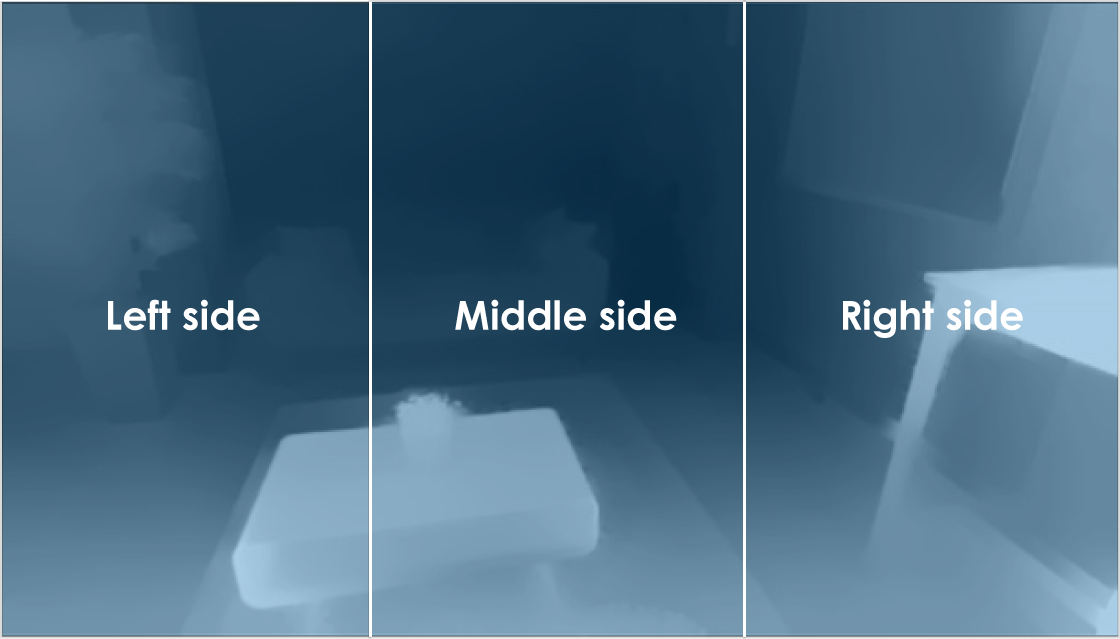
\includegraphics[width=0.8\textwidth]{images/image_division.png}
    \caption{Διαίρεση της εικόνας βάθους σε 3 τμήματα}
    \label{fig:image-division}
\end{figure}
\newpage
\begin{figure}[H]
    \centering
    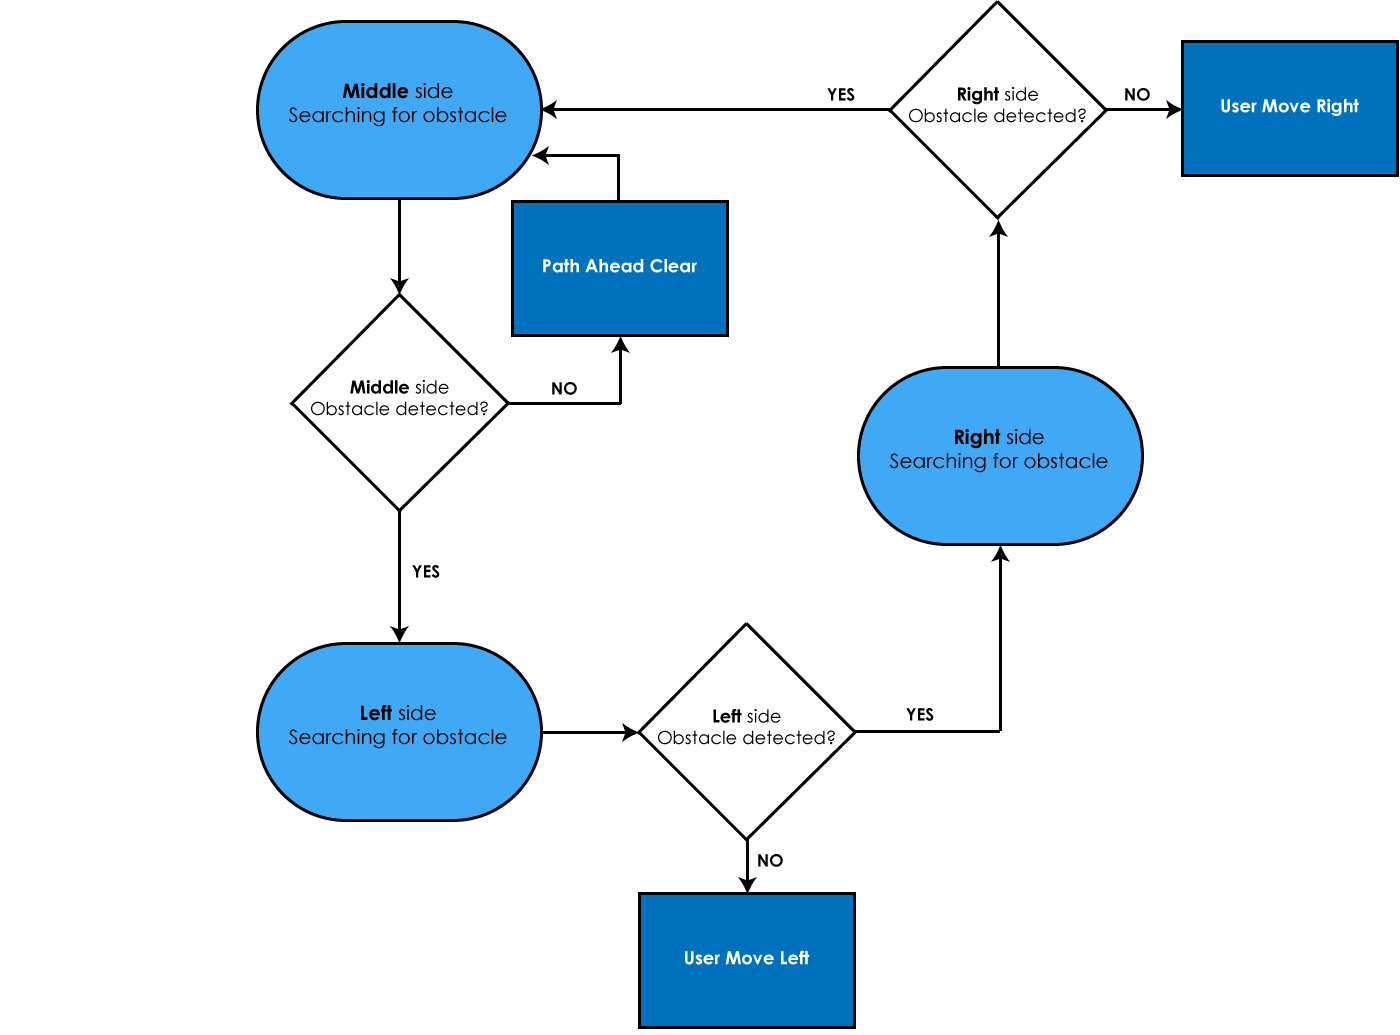
\includegraphics[width=\textwidth]{images/flow_obstacle_detector.png}
    \caption{Overview αλγορίθμου εντοπισμού εμποδίων}
    \label{fig:obstacle-flow}
\end{figure}

\section{Επικοινωνία μεταξύ των συσκευών}
Σύμφωνα με την αρχιτεκτονική του προτεινόμενου συστήματος, που παρουσιάστηκε στο σχήμα \ref{fig:architecture}, απαιτείται η επικοινωνία μεταξύ του smartphone του χρήστη και της μονάδας επεξεργασίας, δηλαδή του Raspberry Pi. Το smartphone αποτελεί το μέσο παροχής ανάδρασης στον χρήστη, μέσα από το οποίο δέχεται ειδοποιήσεις σχετικά με την διαδρομή που πρέπει να ακολουθήσει, την ύπαρξη εμποδίων και την δυνατότητα διάσχισης μιας διάβασης πεζών. Επομένως, είναι απαραίτητη η διασύνδεση της επεξεργαστικής μονάδας, που υλοποιεί τους αλγορίθμους επεξεργασίας εικόνας, με την μονάδα παροχής ανάδρασης. Πιο συγκεκριμένα, το Raspberry Pi στέλνει συγκεκριμένα σήματα ελέγχου στην smartphone, τα οποία ερμηνεύονται κατάλληλα από την εφαρμογή Android και μεταφράζονται στα αντίστοιχα μοτίβα δονήσεων.

\subsection{Απαιτήσεις συστήματος}
Η βασική προϋπόθεση είναι η ασύρματη επικοινωνία, η οποία να επιτρέπει την αμφίδρομη αποστολή/λήψη μηνυμάτων από τις δύο πλευρές. Η κύρια ροή μηνυμάτων είναι από το Raspberry Pi προς το smartphone, ωστόσο είναι αναγκαία και η αντίστροφη διαδρομή, από το smartphone προς το Raspberry Pi, για την λήψη μηνυμάτων επιβεβαίωσης (confirmation messages).

Η αρχική σκέψη του συγγραφέα ήταν η υλοποίηση μιας αμφίδρομης σύνδεσης Bluetooth μεταξύ των δύο συσκευών. Κάτι τέτοιο αποδείχθηκε αρκετά προβληματικό, ωστόσο, αφού τόσο τόσο το Raspberry Pi 4 όσο και το smartphone χρησιμοποιούσαν το πρωτόκολλο Bluetooth 5, το οποίο είναι αρκετά δύσχρηστο για περιπτώσεις όπου χρειάζεται η υλοποίηση μιας απλής σύνδεσης. Επιπλέον, η ξεχωριστή υλοποίηση της Bluetooth σύνδεσης τόσο σε C++ (Raspberry Pi) όσο και σε Java (Android App), αποδείχθηκε πολύ χρονοβόρα, οπότε απορρίφθηκε η λύση του Bluetooth. Η εναλλακτική που επιλέχθηκε ήταν η χρήση του \emph{δικτυακού προγραμματισμού (socket programming)}.

\subsection{Socket Communication}
Η υλοποίηση μιας ασύρματης σύνδεσης με χρήση των λεγόμενων sockets απαιτεί την ύπαρξη ενός τοπικού δικτύου, στο οποίο να είναι συνδεδεμένες οι συσκευές που πρόκειται να επικοινωνήσουν. Για την εγκαθίδρυση ενός τοπικού δικτύου συνδέουμε και τις δύο συσκευές (smartphone \& raspberry pi) σε ένα δίκτυο Wifi. Για τις ανάγκες της διπλωματικής εργασίας οι δύο συσκευές συνδέθηκαν σε ένα δίκτυο wifi-hotspot που παρεχόταν από ένα τρίτο smartphone. Μέσω του ίδιου δικτύου οι συσκευές είχαν πρόσβαση στο διαδίκτυο. Παρακάτω αναλύεται περισσότερο η δομή μιας σύνδεσης μέσω sockets \cite{wiki:sockets}.

\subsubsection{Sockets}
Τα sockets (ή αλλιώς \emph{υποδοχές} στα ελληνικά) παρέχουν σημειακή, αμφίδρομη επικοινωνία μεταξύ διεργασιών, συνήθως -αλλά όχι απαραίτητα- μέσω δικτύου. Αποτελούν μια πολύ ευέλικτη και θεμελιώδη μέθοδο δικτυακής επικοινωνίας μεταξύ διεργασιών ή συστημάτων. Ένα socket είναι μια τερματική σύνδεση η οποία μπορεί να λάβει ένα όνομα (name). Επίσης έχει ένα τύπο (type) και σχετίζεται με μια ή περισσότερες διεργασίες. Τα sockets, ανάλογα με την εφαρμογή που εξυπηρετούν, χαρακτηρίζονται από ένα πρωτόκολλο. Όταν τα sockets χρησιμοποιούνται για επικοινωνία μέσω ενός δικτύου, όπως το internet, αξιοποιούν το πρωτόκολλο επικοινωνίας TCP/IP. Η διεύθυνση ενός socket στο internet αποτελείται από μια διεύθυνση IP και έναν αριθμό θύρας (port).

\subsubsection{Τύποι sockets: TCP/UDP}
Για να γίνει επικοινωνία μεταξύ δύο τερματικών σημείων (endpoints) πρέπει αυτά να χρησιμοποιούν sockets του ίδιου τύπου. Οι δύο βασικοί και πιο διαδεδομένοι τύποι sockets είναι οι ακόλουθοι:
\begin{itemize}
    \item \emph{Stream socket}: Παρέχει αμφίδρομη, ακολουθιακή, αξιόπιστη και μη-επαναλαμβανόμενη ροή δεδομένων χωρίς καθορισμένα όρια μηνύματος. Η επικοινωνία μοιάζει με τηλεφωνική επικοινωνία και χρησιμοποιεί το πρωτόκολλο TCP.
    \item \emph{Datagram socket}: Υποστηρίζει αμφίδρομη ροή μηνυμάτων (datagrams). Η σειρά αποστολής και παραλαβής μηνυμάτων μπορεί να μην είναι  ακολουθιακή. Τα όρια των μηνυμάτων είναι καθορισμένα. Η επικοινωνία μοιάζει με ανταλλαγή επιστολών μέσω ταχυδρομείου και χρησιμοποιεί το πρωτόκολλο UDP.
\end{itemize}
Η σύνδεση που υλοποιήθηκε στα πλαίσια της διπλωματικής χρησιμοποιεί τα stream sockets, που βασίζονται στο TCP, επειδή είναι αναγκαία η αξιόπιστη και μη-επαναλαμβανόμενη μετάδοση των σημάτων ελέγχου από το Raspberry Pi προς το smartphone.

\subsection{Server/Client}
Η επικοινωνία ακολουθεί το μοντέλο εξυπηρετητή/πελάτη (server/client), δηλαδή το ένα τερματικό σημείο λειτουργεί ως εξυπηρετητής και είναι υπεύθυνο για την δημιουργία της σύνδεσης, ενώ το άλλο λειτουργεί ως πελάτης και συνδέεται στην σύνδεση που έχει δημιουργηθεί από έναν εξυπηρετητή. Είναι δυνατόν να υπάρχουν πολλοί διαφορετικοί πελάτες που συνδέονται στον ίδιο εξυπηρετητή και αφού εγκαθιδρυθεί η σύνδεση, τότε η επικοινωνία γίνεται και προς τις δύο πλευρές. Μια σύνδεση μέσω sockets μπορεί να τερματιστεί και από τις δύο πλευρές.

\subsubsection{Server}
Τον ρόλο του server λαμβάνει το Raspberry Pi, δηλαδή είναι υπεύθυνο για την δημιουργία της σύνδεσης. Τα βήματα που υλοποιεί ένας server για τη σύνδεση είναι τα εξής:
\begin{enumerate}
    \item Δημιουργεί ένα socket.
    \item Δεσμεύει το socket με την επιθυμητή δικτυακή διεύθυνση του τελικού σημείου.
    \item Ζητά από το λειτουργικό σύστημα να “ακούει” για εισερχόμενες συνδέσεις.
    \item Εισέρχεται σε κατάσταση όπου αναμένει διαρκώς να του παραδώσει μια σύνδεση το λειτουργικό σύστημα.
    \item Αν λάβει αίτημα εισερχόμενης σύνδεσης, τότε στέλνει πίσω μήνυμα επιβεβαίωσης και δημιουργεί την σύνδεση.
\end{enumerate}

\subsubsection{Client}
Τον ρόλο του μοναδικού client παίζει το smartphone του χρήστη με την εγκατεστημένη εφαρμογή Android. Τα βήματα που ακολουθεί ο client για να συνδεθεί σε ένα socket είναι τα εξής:
\begin{enumerate}
    \item Δημιουργεί ένα socket.
    \item Επιλέγει την διεύθυνση IP του server και προσδιορίζει την επιθυμητή θύρα (port).
    \item Υποβάλλει αίτηση σύνδεσης στον server.  
    \item Με το που λάβει το μήνυμα επιβεβαίωσης εγκαθιδρύεται η σύνδεση.
\end{enumerate}

\begin{figure}[H]
    \centering
    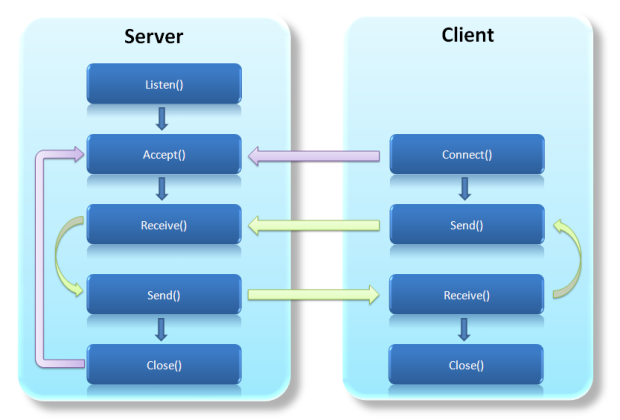
\includegraphics[width=\textwidth]{images/socket_client_server.png}
    \caption{Μοντέλο Server/Client για μια σύνδεση TCP μέσω sockets}
    \label{fig:client-server}
\end{figure}
